\documentclass[twoside]{book}

% Packages required by doxygen
\usepackage{fixltx2e}
\usepackage{calc}
\usepackage{doxygen}
\usepackage[export]{adjustbox} % also loads graphicx
\usepackage{graphicx}
\usepackage[utf8]{inputenc}
\usepackage{makeidx}
\usepackage{multicol}
\usepackage{multirow}
\PassOptionsToPackage{warn}{textcomp}
\usepackage{textcomp}
\usepackage[nointegrals]{wasysym}
\usepackage[table]{xcolor}

% Font selection
\usepackage[T1]{fontenc}
\usepackage[scaled=.90]{helvet}
\usepackage{courier}
\usepackage{amssymb}
\usepackage{sectsty}
\renewcommand{\familydefault}{\sfdefault}
\allsectionsfont{%
  \fontseries{bc}\selectfont%
  \color{darkgray}%
}
\renewcommand{\DoxyLabelFont}{%
  \fontseries{bc}\selectfont%
  \color{darkgray}%
}
\newcommand{\+}{\discretionary{\mbox{\scriptsize$\hookleftarrow$}}{}{}}

% Page & text layout
\usepackage{geometry}
\geometry{%
  a4paper,%
  top=2.5cm,%
  bottom=2.5cm,%
  left=2.5cm,%
  right=2.5cm%
}
\tolerance=750
\hfuzz=15pt
\hbadness=750
\setlength{\emergencystretch}{15pt}
\setlength{\parindent}{0cm}
\setlength{\parskip}{3ex plus 2ex minus 2ex}
\makeatletter
\renewcommand{\paragraph}{%
  \@startsection{paragraph}{4}{0ex}{-1.0ex}{1.0ex}{%
    \normalfont\normalsize\bfseries\SS@parafont%
  }%
}
\renewcommand{\subparagraph}{%
  \@startsection{subparagraph}{5}{0ex}{-1.0ex}{1.0ex}{%
    \normalfont\normalsize\bfseries\SS@subparafont%
  }%
}
\makeatother

% Headers & footers
\usepackage{fancyhdr}
\pagestyle{fancyplain}
\fancyhead[LE]{\fancyplain{}{\bfseries\thepage}}
\fancyhead[CE]{\fancyplain{}{}}
\fancyhead[RE]{\fancyplain{}{\bfseries\leftmark}}
\fancyhead[LO]{\fancyplain{}{\bfseries\rightmark}}
\fancyhead[CO]{\fancyplain{}{}}
\fancyhead[RO]{\fancyplain{}{\bfseries\thepage}}
\fancyfoot[LE]{\fancyplain{}{}}
\fancyfoot[CE]{\fancyplain{}{}}
\fancyfoot[RE]{\fancyplain{}{\bfseries\scriptsize Generated by Doxygen }}
\fancyfoot[LO]{\fancyplain{}{\bfseries\scriptsize Generated by Doxygen }}
\fancyfoot[CO]{\fancyplain{}{}}
\fancyfoot[RO]{\fancyplain{}{}}
\renewcommand{\footrulewidth}{0.4pt}
\renewcommand{\chaptermark}[1]{%
  \markboth{#1}{}%
}
\renewcommand{\sectionmark}[1]{%
  \markright{\thesection\ #1}%
}

% Indices & bibliography
\usepackage{natbib}
\usepackage[titles]{tocloft}
\setcounter{tocdepth}{3}
\setcounter{secnumdepth}{5}
\makeindex

% Hyperlinks (required, but should be loaded last)
\usepackage{ifpdf}
\ifpdf
  \usepackage[pdftex,pagebackref=true]{hyperref}
\else
  \usepackage[ps2pdf,pagebackref=true]{hyperref}
\fi
\hypersetup{%
  colorlinks=true,%
  linkcolor=blue,%
  citecolor=blue,%
  unicode%
}

% Custom commands
\newcommand{\clearemptydoublepage}{%
  \newpage{\pagestyle{empty}\cleardoublepage}%
}

\usepackage{caption}
\captionsetup{labelsep=space,justification=centering,font={bf},singlelinecheck=off,skip=4pt,position=top}

%===== C O N T E N T S =====

\begin{document}

% Titlepage & ToC
\hypersetup{pageanchor=false,
             bookmarksnumbered=true,
             pdfencoding=unicode
            }
\pagenumbering{roman}
\begin{titlepage}
\vspace*{7cm}
\begin{center}%
{\Large Multilayer\+Network Model }\\
\vspace*{1cm}
{\large Generated by Doxygen 1.8.11}\\
\end{center}
\end{titlepage}
\clearemptydoublepage
\tableofcontents
\clearemptydoublepage
\pagenumbering{arabic}
\hypersetup{pageanchor=true}

%--- Begin generated contents ---
\chapter{Hierarchical Index}
\section{Class Hierarchy}
This inheritance list is sorted roughly, but not completely, alphabetically\+:\begin{DoxyCompactList}
\item \contentsline{section}{Ez\+Aquarii\+:\+:Parser\+:\+:basic\+\_\+symbol$<$ by\+\_\+state $>$}{\pageref{structEzAquarii_1_1Parser_1_1basic__symbol}}{}
\item \contentsline{section}{Ez\+Aquarii\+:\+:Parser\+:\+:by\+\_\+type}{\pageref{structEzAquarii_1_1Parser_1_1by__type}}{}
\item \contentsline{section}{Calculation\+Node}{\pageref{classCalculationNode}}{}
\begin{DoxyCompactList}
\item \contentsline{section}{C\+N\+Add}{\pageref{classCNAdd}}{}
\item \contentsline{section}{C\+N\+Constant}{\pageref{classCNConstant}}{}
\item \contentsline{section}{C\+N\+Divide}{\pageref{classCNDivide}}{}
\item \contentsline{section}{C\+N\+Id}{\pageref{classCNId}}{}
\item \contentsline{section}{C\+N\+Multiply}{\pageref{classCNMultiply}}{}
\item \contentsline{section}{C\+N\+Negate}{\pageref{classCNNegate}}{}
\item \contentsline{section}{C\+N\+Power}{\pageref{classCNPower}}{}
\item \contentsline{section}{C\+N\+Subtract}{\pageref{classCNSubtract}}{}
\end{DoxyCompactList}
\item \contentsline{section}{Dynamical\+Equation}{\pageref{classDynamicalEquation}}{}
\item \contentsline{section}{Genetic\+Algorithm\+Controller}{\pageref{classGeneticAlgorithmController}}{}
\item \contentsline{section}{I\+Downward\+Influence}{\pageref{classIDownwardInfluence}}{}
\begin{DoxyCompactList}
\item \contentsline{section}{Downward\+Influence\+Impl}{\pageref{classDownwardInfluenceImpl}}{}
\end{DoxyCompactList}
\item \contentsline{section}{I\+Dynamical\+Equation\+Generator}{\pageref{classIDynamicalEquationGenerator}}{}
\begin{DoxyCompactList}
\item \contentsline{section}{Dynamical\+Equation\+Generator\+Simple\+Impl}{\pageref{classDynamicalEquationGeneratorSimpleImpl}}{}
\end{DoxyCompactList}
\item \contentsline{section}{I\+Initial\+Condition\+Generator}{\pageref{classIInitialConditionGenerator}}{}
\begin{DoxyCompactList}
\item \contentsline{section}{Initial\+Condition\+Generator\+Impl}{\pageref{classInitialConditionGeneratorImpl}}{}
\end{DoxyCompactList}
\item \contentsline{section}{Ez\+Aquarii\+:\+:Interpreter}{\pageref{classEzAquarii_1_1Interpreter}}{}
\item \contentsline{section}{I\+Structure\+Generator}{\pageref{classIStructureGenerator}}{}
\begin{DoxyCompactList}
\item \contentsline{section}{Structure\+Generator\+Impl}{\pageref{classStructureGeneratorImpl}}{}
\end{DoxyCompactList}
\item \contentsline{section}{I\+Upward\+Influence}{\pageref{classIUpwardInfluence}}{}
\begin{DoxyCompactList}
\item \contentsline{section}{Upward\+Influence\+Impl}{\pageref{classUpwardInfluenceImpl}}{}
\end{DoxyCompactList}
\item \contentsline{section}{I\+Vector\+Field\+Reconfiguration}{\pageref{classIVectorFieldReconfiguration}}{}
\begin{DoxyCompactList}
\item \contentsline{section}{Vector\+Field\+Reconfiguration\+Impl}{\pageref{classVectorFieldReconfigurationImpl}}{}
\end{DoxyCompactList}
\item \contentsline{section}{Layer}{\pageref{classLayer}}{}
\item \contentsline{section}{Ez\+Aquarii\+:\+:location}{\pageref{classEzAquarii_1_1location}}{}
\item \contentsline{section}{Multilayer\+Network}{\pageref{classMultilayerNetwork}}{}
\item \contentsline{section}{Network}{\pageref{classNetwork}}{}
\item \contentsline{section}{Network\+Modifier}{\pageref{classNetworkModifier}}{}
\item \contentsline{section}{Network\+Population\+Element}{\pageref{classNetworkPopulationElement}}{}
\item \contentsline{section}{Node}{\pageref{classNode}}{}
\item \contentsline{section}{Ode\+Wrapper}{\pageref{classOdeWrapper}}{}
\item \contentsline{section}{Ode\+Wrapper\+At\+State}{\pageref{classOdeWrapperAtState}}{}
\item \contentsline{section}{Ez\+Aquarii\+:\+:Parser}{\pageref{classEzAquarii_1_1Parser}}{}
\item \contentsline{section}{Ez\+Aquarii\+:\+:position}{\pageref{classEzAquarii_1_1position}}{}
\item runtime\+\_\+error\begin{DoxyCompactList}
\item \contentsline{section}{Ez\+Aquarii\+:\+:Parser\+:\+:syntax\+\_\+error}{\pageref{structEzAquarii_1_1Parser_1_1syntax__error}}{}
\end{DoxyCompactList}
\item \contentsline{section}{Ez\+Aquarii\+:\+:slice$<$ T, S $>$}{\pageref{classEzAquarii_1_1slice}}{}
\item \contentsline{section}{Ez\+Aquarii\+:\+:stack$<$ T, S $>$}{\pageref{classEzAquarii_1_1stack}}{}
\item \contentsline{section}{Ez\+Aquarii\+:\+:stack$<$ stack\+\_\+symbol\+\_\+type $>$}{\pageref{classEzAquarii_1_1stack}}{}
\item \contentsline{section}{Ez\+Aquarii\+:\+:Parser\+:\+:token}{\pageref{structEzAquarii_1_1Parser_1_1token}}{}
\item \contentsline{section}{Ez\+Aquarii\+:\+:Parser\+:\+:union\+\_\+type}{\pageref{unionEzAquarii_1_1Parser_1_1union__type}}{}
\item \contentsline{section}{Ez\+Aquarii\+:\+:variant$<$ S $>$}{\pageref{structEzAquarii_1_1variant}}{}
\item \contentsline{section}{Ez\+Aquarii\+:\+:variant$<$ sizeof(union\+\_\+type)$>$}{\pageref{structEzAquarii_1_1variant}}{}
\item \contentsline{section}{Vector\+Field}{\pageref{classVectorField}}{}
\item \contentsline{section}{Vector\+Field\+Point}{\pageref{classVectorFieldPoint}}{}
\item \contentsline{section}{yy\+\_\+buffer\+\_\+state}{\pageref{structyy__buffer__state}}{}
\item \contentsline{section}{yy\+\_\+trans\+\_\+info}{\pageref{structyy__trans__info}}{}
\item yy\+Flex\+Lexer\begin{DoxyCompactList}
\item \contentsline{section}{Ez\+Aquarii\+:\+:Scanner}{\pageref{classEzAquarii_1_1Scanner}}{}
\end{DoxyCompactList}
\item Base\begin{DoxyCompactList}
\item \contentsline{section}{Ez\+Aquarii\+:\+:Parser\+:\+:basic\+\_\+symbol$<$ Base $>$}{\pageref{structEzAquarii_1_1Parser_1_1basic__symbol}}{}
\end{DoxyCompactList}
\end{DoxyCompactList}

\chapter{Class Index}
\section{Class List}
Here are the classes, structs, unions and interfaces with brief descriptions\+:\begin{DoxyCompactList}
\item\contentsline{section}{\hyperlink{classrapidjson_1_1Allocator}{rapidjson\+::\+Allocator} \\*Concept for allocating, resizing and freeing memory block }{\pageref{classrapidjson_1_1Allocator}}{}
\item\contentsline{section}{\hyperlink{structGenericValue_1_1ArrayData}{Generic\+Value$<$ Encoding, Allocator $>$\+::\+Array\+Data} }{\pageref{structGenericValue_1_1ArrayData}}{}
\item\contentsline{section}{\hyperlink{structASCII}{A\+S\+C\+I\+I$<$ Char\+Type $>$} \\*\hyperlink{structASCII}{A\+S\+C\+II} encoding }{\pageref{structASCII}}{}
\item\contentsline{section}{\hyperlink{structAutoUTF}{Auto\+U\+T\+F$<$ Char\+Type $>$} \\*Dynamically select encoding according to stream\textquotesingle{}s runtime-\/specified U\+TF encoding type }{\pageref{structAutoUTF}}{}
\item\contentsline{section}{\hyperlink{classAutoUTFInputStream}{Auto\+U\+T\+F\+Input\+Stream$<$ Char\+Type, Input\+Byte\+Stream $>$} \\*Input stream wrapper with dynamically bound encoding and automatic encoding detection }{\pageref{classAutoUTFInputStream}}{}
\item\contentsline{section}{\hyperlink{classAutoUTFOutputStream}{Auto\+U\+T\+F\+Output\+Stream$<$ Char\+Type, Output\+Byte\+Stream $>$} \\*Output stream wrapper with dynamically bound encoding and automatic encoding detection }{\pageref{classAutoUTFOutputStream}}{}
\item\contentsline{section}{\hyperlink{structBaseReaderHandler}{Base\+Reader\+Handler$<$ Encoding, Derived $>$} \\*Default implementation of Handler }{\pageref{structBaseReaderHandler}}{}
\item\contentsline{section}{\hyperlink{structEquationParser_1_1Parser_1_1basic__symbol}{Equation\+Parser\+::\+Parser\+::basic\+\_\+symbol$<$ Base $>$} }{\pageref{structEquationParser_1_1Parser_1_1basic__symbol}}{}
\item\contentsline{section}{\hyperlink{classBasicIStreamWrapper}{Basic\+I\+Stream\+Wrapper$<$ Stream\+Type $>$} \\*Wrapper of {\ttfamily std\+::basic\+\_\+istream} into Rapid\+J\+S\+ON\textquotesingle{}s Stream concept }{\pageref{classBasicIStreamWrapper}}{}
\item\contentsline{section}{\hyperlink{classBasicOStreamWrapper}{Basic\+O\+Stream\+Wrapper$<$ Stream\+Type $>$} \\*Wrapper of {\ttfamily std\+::basic\+\_\+ostream} into Rapid\+J\+S\+ON\textquotesingle{}s Stream concept }{\pageref{classBasicOStreamWrapper}}{}
\item\contentsline{section}{\hyperlink{classinternal_1_1BigInteger}{internal\+::\+Big\+Integer} }{\pageref{classinternal_1_1BigInteger}}{}
\item\contentsline{section}{\hyperlink{structEquationParser_1_1Parser_1_1by__type}{Equation\+Parser\+::\+Parser\+::by\+\_\+type} \\*Type access provider for token (enum) based symbols }{\pageref{structEquationParser_1_1Parser_1_1by__type}}{}
\item\contentsline{section}{\hyperlink{classCalculationNode}{Calculation\+Node} }{\pageref{classCalculationNode}}{}
\item\contentsline{section}{\hyperlink{classCNAdd}{C\+N\+Add} }{\pageref{classCNAdd}}{}
\item\contentsline{section}{\hyperlink{classCNConstant}{C\+N\+Constant} }{\pageref{classCNConstant}}{}
\item\contentsline{section}{\hyperlink{classCNDivide}{C\+N\+Divide} }{\pageref{classCNDivide}}{}
\item\contentsline{section}{\hyperlink{classCNId}{C\+N\+Id} }{\pageref{classCNId}}{}
\item\contentsline{section}{\hyperlink{classCNMultiply}{C\+N\+Multiply} }{\pageref{classCNMultiply}}{}
\item\contentsline{section}{\hyperlink{classCNNegate}{C\+N\+Negate} }{\pageref{classCNNegate}}{}
\item\contentsline{section}{\hyperlink{classCNPower}{C\+N\+Power} }{\pageref{classCNPower}}{}
\item\contentsline{section}{\hyperlink{classCNSubtract}{C\+N\+Subtract} }{\pageref{classCNSubtract}}{}
\item\contentsline{section}{\hyperlink{classCrtAllocator}{Crt\+Allocator} \\*C-\/runtime library allocator }{\pageref{classCrtAllocator}}{}
\item\contentsline{section}{\hyperlink{classCursorStreamWrapper}{Cursor\+Stream\+Wrapper$<$ Input\+Stream, Encoding $>$} \\*Cursor stream wrapper for counting line and column number if error exists }{\pageref{classCursorStreamWrapper}}{}
\item\contentsline{section}{\hyperlink{unionGenericValue_1_1Data}{Generic\+Value$<$ Encoding, Allocator $>$\+::\+Data} }{\pageref{unionGenericValue_1_1Data}}{}
\item\contentsline{section}{\hyperlink{classinternal_1_1DecodedStream}{internal\+::\+Decoded\+Stream$<$ Source\+Stream, Encoding $>$} }{\pageref{classinternal_1_1DecodedStream}}{}
\item\contentsline{section}{\hyperlink{structinternal_1_1DiyFp}{internal\+::\+Diy\+Fp} }{\pageref{structinternal_1_1DiyFp}}{}
\item\contentsline{section}{\hyperlink{classinternal_1_1Double}{internal\+::\+Double} }{\pageref{classinternal_1_1Double}}{}
\item\contentsline{section}{\hyperlink{classDownwardInfluenceImpl}{Downward\+Influence\+Impl} }{\pageref{classDownwardInfluenceImpl}}{}
\item\contentsline{section}{\hyperlink{classDynamicalEquation}{Dynamical\+Equation} }{\pageref{classDynamicalEquation}}{}
\item\contentsline{section}{\hyperlink{classDynamicalEquationGeneratorSimpleImpl}{Dynamical\+Equation\+Generator\+Simple\+Impl} }{\pageref{classDynamicalEquationGeneratorSimpleImpl}}{}
\item\contentsline{section}{\hyperlink{classEncodedInputStream}{Encoded\+Input\+Stream$<$ Encoding, Input\+Byte\+Stream $>$} \\*Input byte stream wrapper with a statically bound encoding }{\pageref{classEncodedInputStream}}{}
\item\contentsline{section}{\hyperlink{classEncodedInputStream_3_01UTF8_3_4_00_01MemoryStream_01_4}{Encoded\+Input\+Stream$<$ U\+T\+F8$<$$>$, Memory\+Stream $>$} \\*Specialized for \hyperlink{structUTF8}{U\+T\+F8} \hyperlink{structMemoryStream}{Memory\+Stream} }{\pageref{classEncodedInputStream_3_01UTF8_3_4_00_01MemoryStream_01_4}}{}
\item\contentsline{section}{\hyperlink{classEncodedOutputStream}{Encoded\+Output\+Stream$<$ Encoding, Output\+Byte\+Stream $>$} \\*Output byte stream wrapper with statically bound encoding }{\pageref{classEncodedOutputStream}}{}
\item\contentsline{section}{\hyperlink{classrapidjson_1_1Encoding}{rapidjson\+::\+Encoding} \\*Concept for encoding of Unicode characters }{\pageref{classrapidjson_1_1Encoding}}{}
\item\contentsline{section}{\hyperlink{classFileReadStream}{File\+Read\+Stream} \\*File byte stream for input using fread() }{\pageref{classFileReadStream}}{}
\item\contentsline{section}{\hyperlink{classFileWriteStream}{File\+Write\+Stream} \\*Wrapper of C file stream for input using fread() }{\pageref{classFileWriteStream}}{}
\item\contentsline{section}{\hyperlink{structGenericValue_1_1Flag}{Generic\+Value$<$ Encoding, Allocator $>$\+::\+Flag} }{\pageref{structGenericValue_1_1Flag}}{}
\item\contentsline{section}{\hyperlink{classGenericArray}{Generic\+Array$<$ Const, Value\+T $>$} \\*Helper class for accessing Value of array type }{\pageref{classGenericArray}}{}
\item\contentsline{section}{\hyperlink{classGenericDocument}{Generic\+Document$<$ Encoding, Allocator, Stack\+Allocator $>$} \\*A document for parsing J\+S\+ON text as D\+OM }{\pageref{classGenericDocument}}{}
\item\contentsline{section}{\hyperlink{structGenericInsituStringStream}{Generic\+Insitu\+String\+Stream$<$ Encoding $>$} \\*A read-\/write string stream }{\pageref{structGenericInsituStringStream}}{}
\item\contentsline{section}{\hyperlink{structGenericMember}{Generic\+Member$<$ Encoding, Allocator $>$} \\*Name-\/value pair in a J\+S\+ON object value }{\pageref{structGenericMember}}{}
\item\contentsline{section}{\hyperlink{classGenericMemberIterator}{Generic\+Member\+Iterator$<$ Const, Encoding, Allocator $>$} \\*(Constant) member iterator for a J\+S\+ON object value }{\pageref{classGenericMemberIterator}}{}
\item\contentsline{section}{\hyperlink{structGenericMemoryBuffer}{Generic\+Memory\+Buffer$<$ Allocator $>$} \\*Represents an in-\/memory output byte stream }{\pageref{structGenericMemoryBuffer}}{}
\item\contentsline{section}{\hyperlink{classGenericObject}{Generic\+Object$<$ Const, Value\+T $>$} \\*Helper class for accessing Value of object type }{\pageref{classGenericObject}}{}
\item\contentsline{section}{\hyperlink{classGenericPointer}{Generic\+Pointer$<$ Value\+Type, Allocator $>$} \\*Represents a J\+S\+ON Pointer. Use Pointer for \hyperlink{structUTF8}{U\+T\+F8} encoding and default allocator }{\pageref{classGenericPointer}}{}
\item\contentsline{section}{\hyperlink{classGenericReader}{Generic\+Reader$<$ Source\+Encoding, Target\+Encoding, Stack\+Allocator $>$} \\*S\+A\+X-\/style J\+S\+ON parser. Use \hyperlink{reader_8h_a84f3b66a66647f4ac4267078359188ba}{Reader} for \hyperlink{structUTF8}{U\+T\+F8} encoding and default allocator }{\pageref{classGenericReader}}{}
\item\contentsline{section}{\hyperlink{classinternal_1_1GenericRegex}{internal\+::\+Generic\+Regex$<$ Encoding, Allocator $>$} \\*Regular expression engine with subset of E\+C\+M\+Ascript grammar }{\pageref{classinternal_1_1GenericRegex}}{}
\item\contentsline{section}{\hyperlink{classinternal_1_1GenericRegexSearch}{internal\+::\+Generic\+Regex\+Search$<$ Regex\+Type, Allocator $>$} }{\pageref{classinternal_1_1GenericRegexSearch}}{}
\item\contentsline{section}{\hyperlink{classGenericSchemaDocument}{Generic\+Schema\+Document$<$ Value\+T, Allocator $>$} \\*J\+S\+ON schema document }{\pageref{classGenericSchemaDocument}}{}
\item\contentsline{section}{\hyperlink{classGenericSchemaValidator}{Generic\+Schema\+Validator$<$ Schema\+Document\+Type, Output\+Handler, State\+Allocator $>$} \\*J\+S\+ON Schema Validator }{\pageref{classGenericSchemaValidator}}{}
\item\contentsline{section}{\hyperlink{classGenericStreamWrapper}{Generic\+Stream\+Wrapper$<$ Input\+Stream, Encoding $>$} \\*A Stream Wrapper }{\pageref{classGenericStreamWrapper}}{}
\item\contentsline{section}{\hyperlink{classGenericStringBuffer}{Generic\+String\+Buffer$<$ Encoding, Allocator $>$} \\*Represents an in-\/memory output stream }{\pageref{classGenericStringBuffer}}{}
\item\contentsline{section}{\hyperlink{structGenericStringRef}{Generic\+String\+Ref$<$ Char\+Type $>$} \\*Reference to a constant string (not taking a copy) }{\pageref{structGenericStringRef}}{}
\item\contentsline{section}{\hyperlink{structGenericStringStream}{Generic\+String\+Stream$<$ Encoding $>$} \\*Read-\/only string stream }{\pageref{structGenericStringStream}}{}
\item\contentsline{section}{\hyperlink{classGenericValue}{Generic\+Value$<$ Encoding, Allocator $>$} \\*Represents a J\+S\+ON value. Use Value for \hyperlink{structUTF8}{U\+T\+F8} encoding and default allocator }{\pageref{classGenericValue}}{}
\item\contentsline{section}{\hyperlink{classGeneticAlgorithmController}{Genetic\+Algorithm\+Controller} }{\pageref{classGeneticAlgorithmController}}{}
\item\contentsline{section}{\hyperlink{classrapidjson_1_1Handler}{rapidjson\+::\+Handler} \\*Concept for receiving events from \hyperlink{classGenericReader}{Generic\+Reader} upon parsing. The functions return true if no error occurs. If they return false, the event publisher should terminate the process }{\pageref{classrapidjson_1_1Handler}}{}
\item\contentsline{section}{\hyperlink{classinternal_1_1Hasher}{internal\+::\+Hasher$<$ Encoding, Allocator $>$} }{\pageref{classinternal_1_1Hasher}}{}
\item\contentsline{section}{\hyperlink{structGenericValue_1_1Number_1_1I}{Generic\+Value$<$ Encoding, Allocator $>$\+::\+Number\+::I} }{\pageref{structGenericValue_1_1Number_1_1I}}{}
\item\contentsline{section}{\hyperlink{classIDownwardInfluence}{I\+Downward\+Influence} }{\pageref{classIDownwardInfluence}}{}
\item\contentsline{section}{\hyperlink{classIDynamicalEquationGenerator}{I\+Dynamical\+Equation\+Generator} }{\pageref{classIDynamicalEquationGenerator}}{}
\item\contentsline{section}{\hyperlink{classIGenericRemoteSchemaDocumentProvider}{I\+Generic\+Remote\+Schema\+Document\+Provider$<$ Schema\+Document\+Type $>$} }{\pageref{classIGenericRemoteSchemaDocumentProvider}}{}
\item\contentsline{section}{\hyperlink{classIInitialConditionGenerator}{I\+Initial\+Condition\+Generator} }{\pageref{classIInitialConditionGenerator}}{}
\item\contentsline{section}{\hyperlink{structimaxdiv__t}{imaxdiv\+\_\+t} }{\pageref{structimaxdiv__t}}{}
\item\contentsline{section}{\hyperlink{classInitialConditionGeneratorImpl}{Initial\+Condition\+Generator\+Impl} }{\pageref{classInitialConditionGeneratorImpl}}{}
\item\contentsline{section}{\hyperlink{classEquationParser_1_1Interpreter}{Equation\+Parser\+::\+Interpreter} }{\pageref{classEquationParser_1_1Interpreter}}{}
\item\contentsline{section}{\hyperlink{classinternal_1_1ISchemaStateFactory}{internal\+::\+I\+Schema\+State\+Factory$<$ Schema\+Type $>$} }{\pageref{classinternal_1_1ISchemaStateFactory}}{}
\item\contentsline{section}{\hyperlink{classinternal_1_1ISchemaValidator}{internal\+::\+I\+Schema\+Validator} }{\pageref{classinternal_1_1ISchemaValidator}}{}
\item\contentsline{section}{\hyperlink{structinternal_1_1IsGenericValue}{internal\+::\+Is\+Generic\+Value$<$ T $>$} }{\pageref{structinternal_1_1IsGenericValue}}{}
\item\contentsline{section}{\hyperlink{structinternal_1_1IsGenericValueImpl}{internal\+::\+Is\+Generic\+Value\+Impl$<$ T, Encoding, Allocator $>$} }{\pageref{structinternal_1_1IsGenericValueImpl}}{}
\item\contentsline{section}{\hyperlink{structinternal_1_1IsGenericValueImpl_3_01T_00_01typename_01Void_3_01typename_01T_1_1EncodingType794abcc01fcce01e300668fa57e4d036}{internal\+::\+Is\+Generic\+Value\+Impl$<$ T, typename Void$<$ typename T\+::\+Encoding\+Type $>$\+::\+Type, typename Void$<$ typename T\+::\+Allocator\+Type $>$\+::\+Type $>$} }{\pageref{structinternal_1_1IsGenericValueImpl_3_01T_00_01typename_01Void_3_01typename_01T_1_1EncodingType794abcc01fcce01e300668fa57e4d036}}{}
\item\contentsline{section}{\hyperlink{classIStructureGenerator}{I\+Structure\+Generator} }{\pageref{classIStructureGenerator}}{}
\item\contentsline{section}{\hyperlink{classIUpwardInfluence}{I\+Upward\+Influence} }{\pageref{classIUpwardInfluence}}{}
\item\contentsline{section}{\hyperlink{classIVectorFieldReconfiguration}{I\+Vector\+Field\+Reconfiguration} }{\pageref{classIVectorFieldReconfiguration}}{}
\item\contentsline{section}{\hyperlink{classLayer}{Layer} }{\pageref{classLayer}}{}
\item\contentsline{section}{\hyperlink{structWriter_1_1Level}{Writer$<$ Output\+Stream, Source\+Encoding, Target\+Encoding, Stack\+Allocator, write\+Flags $>$\+::\+Level} \\*Information for each nested level }{\pageref{structWriter_1_1Level}}{}
\item\contentsline{section}{\hyperlink{classEquationParser_1_1location}{Equation\+Parser\+::location} \\*Abstract a location }{\pageref{classEquationParser_1_1location}}{}
\item\contentsline{section}{\hyperlink{classMemoryPoolAllocator}{Memory\+Pool\+Allocator$<$ Base\+Allocator $>$} \\*Default memory allocator used by the parser and D\+OM }{\pageref{classMemoryPoolAllocator}}{}
\item\contentsline{section}{\hyperlink{structMemoryStream}{Memory\+Stream} \\*Represents an in-\/memory input byte stream }{\pageref{structMemoryStream}}{}
\item\contentsline{section}{\hyperlink{classMultilayerNetwork}{Multilayer\+Network} }{\pageref{classMultilayerNetwork}}{}
\item\contentsline{section}{\hyperlink{classNetwork}{Network} }{\pageref{classNetwork}}{}
\item\contentsline{section}{\hyperlink{classNetworkModifier}{Network\+Modifier} }{\pageref{classNetworkModifier}}{}
\item\contentsline{section}{\hyperlink{classNetworkPopulationElement}{Network\+Population\+Element} }{\pageref{classNetworkPopulationElement}}{}
\item\contentsline{section}{\hyperlink{classNode}{Node} }{\pageref{classNode}}{}
\item\contentsline{section}{\hyperlink{unionGenericValue_1_1Number}{Generic\+Value$<$ Encoding, Allocator $>$\+::\+Number} }{\pageref{unionGenericValue_1_1Number}}{}
\item\contentsline{section}{\hyperlink{structGenericValue_1_1ObjectData}{Generic\+Value$<$ Encoding, Allocator $>$\+::\+Object\+Data} }{\pageref{structGenericValue_1_1ObjectData}}{}
\item\contentsline{section}{\hyperlink{classOdeWrapper}{Ode\+Wrapper} }{\pageref{classOdeWrapper}}{}
\item\contentsline{section}{\hyperlink{classOdeWrapperAtState}{Ode\+Wrapper\+At\+State} }{\pageref{classOdeWrapperAtState}}{}
\item\contentsline{section}{\hyperlink{classEquationParser_1_1Parser}{Equation\+Parser\+::\+Parser} \\*A Bison parser }{\pageref{classEquationParser_1_1Parser}}{}
\item\contentsline{section}{\hyperlink{structParseResult}{Parse\+Result} \\*Result of parsing (wraps Parse\+Error\+Code) }{\pageref{structParseResult}}{}
\item\contentsline{section}{\hyperlink{classEquationParser_1_1position}{Equation\+Parser\+::position} \\*Abstract a position }{\pageref{classEquationParser_1_1position}}{}
\item\contentsline{section}{\hyperlink{classPrettyWriter}{Pretty\+Writer$<$ Output\+Stream, Source\+Encoding, Target\+Encoding, Stack\+Allocator, write\+Flags $>$} \\*\hyperlink{classWriter}{Writer} with indentation and spacing }{\pageref{classPrettyWriter}}{}
\item\contentsline{section}{\hyperlink{classEquationParser_1_1Scanner}{Equation\+Parser\+::\+Scanner} }{\pageref{classEquationParser_1_1Scanner}}{}
\item\contentsline{section}{\hyperlink{classinternal_1_1Schema}{internal\+::\+Schema$<$ Schema\+Document\+Type $>$} }{\pageref{classinternal_1_1Schema}}{}
\item\contentsline{section}{\hyperlink{classSchemaValidatingReader}{Schema\+Validating\+Reader$<$ parse\+Flags, Input\+Stream, Source\+Encoding, Schema\+Document\+Type, Stack\+Allocator $>$} \\*A helper class for parsing with validation }{\pageref{classSchemaValidatingReader}}{}
\item\contentsline{section}{\hyperlink{structinternal_1_1SchemaValidationContext}{internal\+::\+Schema\+Validation\+Context$<$ Schema\+Document\+Type $>$} }{\pageref{structinternal_1_1SchemaValidationContext}}{}
\item\contentsline{section}{\hyperlink{structGenericValue_1_1ShortString}{Generic\+Value$<$ Encoding, Allocator $>$\+::\+Short\+String} }{\pageref{structGenericValue_1_1ShortString}}{}
\item\contentsline{section}{\hyperlink{classEquationParser_1_1slice}{Equation\+Parser\+::slice$<$ T, S $>$} \\*Present a slice of the top of a stack }{\pageref{classEquationParser_1_1slice}}{}
\item\contentsline{section}{\hyperlink{classEquationParser_1_1stack}{Equation\+Parser\+::stack$<$ T, S $>$} }{\pageref{classEquationParser_1_1stack}}{}
\item\contentsline{section}{\hyperlink{classinternal_1_1Stack}{internal\+::\+Stack$<$ Allocator $>$} \\*A type-\/unsafe stack for storing different types of data }{\pageref{classinternal_1_1Stack}}{}
\item\contentsline{section}{\hyperlink{classrapidjson_1_1Stream}{rapidjson\+::\+Stream} \\*Concept for reading and writing characters }{\pageref{classrapidjson_1_1Stream}}{}
\item\contentsline{section}{\hyperlink{classinternal_1_1StreamLocalCopy}{internal\+::\+Stream\+Local\+Copy$<$ Stream, int $>$} }{\pageref{classinternal_1_1StreamLocalCopy}}{}
\item\contentsline{section}{\hyperlink{classinternal_1_1StreamLocalCopy_3_01Stream_00_010_01_4}{internal\+::\+Stream\+Local\+Copy$<$ Stream, 0 $>$} \\*Keep reference }{\pageref{classinternal_1_1StreamLocalCopy_3_01Stream_00_010_01_4}}{}
\item\contentsline{section}{\hyperlink{classinternal_1_1StreamLocalCopy_3_01Stream_00_011_01_4}{internal\+::\+Stream\+Local\+Copy$<$ Stream, 1 $>$} \\*Do copy optimization }{\pageref{classinternal_1_1StreamLocalCopy_3_01Stream_00_011_01_4}}{}
\item\contentsline{section}{\hyperlink{structStreamTraits}{Stream\+Traits$<$ Stream $>$} \\*Provides additional information for stream }{\pageref{structStreamTraits}}{}
\item\contentsline{section}{\hyperlink{structStreamTraits_3_01GenericInsituStringStream_3_01Encoding_01_4_01_4}{Stream\+Traits$<$ Generic\+Insitu\+String\+Stream$<$ Encoding $>$ $>$} }{\pageref{structStreamTraits_3_01GenericInsituStringStream_3_01Encoding_01_4_01_4}}{}
\item\contentsline{section}{\hyperlink{structStreamTraits_3_01GenericStringStream_3_01Encoding_01_4_01_4}{Stream\+Traits$<$ Generic\+String\+Stream$<$ Encoding $>$ $>$} }{\pageref{structStreamTraits_3_01GenericStringStream_3_01Encoding_01_4_01_4}}{}
\item\contentsline{section}{\hyperlink{structGenericValue_1_1String}{Generic\+Value$<$ Encoding, Allocator $>$\+::\+String} }{\pageref{structGenericValue_1_1String}}{}
\item\contentsline{section}{\hyperlink{classStructureGeneratorImpl}{Structure\+Generator\+Impl} }{\pageref{classStructureGeneratorImpl}}{}
\item\contentsline{section}{\hyperlink{structEquationParser_1_1Parser_1_1syntax__error}{Equation\+Parser\+::\+Parser\+::syntax\+\_\+error} \\*Syntax errors thrown from user actions }{\pageref{structEquationParser_1_1Parser_1_1syntax__error}}{}
\item\contentsline{section}{\hyperlink{structEquationParser_1_1Parser_1_1token}{Equation\+Parser\+::\+Parser\+::token} \\*Tokens }{\pageref{structEquationParser_1_1Parser_1_1token}}{}
\item\contentsline{section}{\hyperlink{structGenericPointer_1_1Token}{Generic\+Pointer$<$ Value\+Type, Allocator $>$\+::\+Token} \\*A token is the basic units of internal representation }{\pageref{structGenericPointer_1_1Token}}{}
\item\contentsline{section}{\hyperlink{structinternal_1_1TokenHelper}{internal\+::\+Token\+Helper$<$ Stack, Ch $>$} }{\pageref{structinternal_1_1TokenHelper}}{}
\item\contentsline{section}{\hyperlink{structinternal_1_1TokenHelper_3_01Stack_00_01char_01_4}{internal\+::\+Token\+Helper$<$ Stack, char $>$} }{\pageref{structinternal_1_1TokenHelper_3_01Stack_00_01char_01_4}}{}
\item\contentsline{section}{\hyperlink{structTranscoder}{Transcoder$<$ Source\+Encoding, Target\+Encoding $>$} \\*Encoding conversion }{\pageref{structTranscoder}}{}
\item\contentsline{section}{\hyperlink{structTranscoder_3_01Encoding_00_01Encoding_01_4}{Transcoder$<$ Encoding, Encoding $>$} \\*Specialization of \hyperlink{structTranscoder}{Transcoder} with same source and target encoding }{\pageref{structTranscoder_3_01Encoding_00_01Encoding_01_4}}{}
\item\contentsline{section}{\hyperlink{structinternal_1_1TypeHelper}{internal\+::\+Type\+Helper$<$ Value\+Type, T $>$} }{\pageref{structinternal_1_1TypeHelper}}{}
\item\contentsline{section}{\hyperlink{structinternal_1_1TypeHelper_3_01ValueType_00_01bool_01_4}{internal\+::\+Type\+Helper$<$ Value\+Type, bool $>$} }{\pageref{structinternal_1_1TypeHelper_3_01ValueType_00_01bool_01_4}}{}
\item\contentsline{section}{\hyperlink{structinternal_1_1TypeHelper_3_01ValueType_00_01const_01typename_01ValueType_1_1Ch_01_5_01_4}{internal\+::\+Type\+Helper$<$ Value\+Type, const typename Value\+Type\+::\+Ch $\ast$ $>$} }{\pageref{structinternal_1_1TypeHelper_3_01ValueType_00_01const_01typename_01ValueType_1_1Ch_01_5_01_4}}{}
\item\contentsline{section}{\hyperlink{structinternal_1_1TypeHelper_3_01ValueType_00_01double_01_4}{internal\+::\+Type\+Helper$<$ Value\+Type, double $>$} }{\pageref{structinternal_1_1TypeHelper_3_01ValueType_00_01double_01_4}}{}
\item\contentsline{section}{\hyperlink{structinternal_1_1TypeHelper_3_01ValueType_00_01float_01_4}{internal\+::\+Type\+Helper$<$ Value\+Type, float $>$} }{\pageref{structinternal_1_1TypeHelper_3_01ValueType_00_01float_01_4}}{}
\item\contentsline{section}{\hyperlink{structinternal_1_1TypeHelper_3_01ValueType_00_01int_01_4}{internal\+::\+Type\+Helper$<$ Value\+Type, int $>$} }{\pageref{structinternal_1_1TypeHelper_3_01ValueType_00_01int_01_4}}{}
\item\contentsline{section}{\hyperlink{structinternal_1_1TypeHelper_3_01ValueType_00_01int64__t_01_4}{internal\+::\+Type\+Helper$<$ Value\+Type, int64\+\_\+t $>$} }{\pageref{structinternal_1_1TypeHelper_3_01ValueType_00_01int64__t_01_4}}{}
\item\contentsline{section}{\hyperlink{structinternal_1_1TypeHelper_3_01ValueType_00_01typename_01ValueType_1_1Array_01_4}{internal\+::\+Type\+Helper$<$ Value\+Type, typename Value\+Type\+::\+Array $>$} }{\pageref{structinternal_1_1TypeHelper_3_01ValueType_00_01typename_01ValueType_1_1Array_01_4}}{}
\item\contentsline{section}{\hyperlink{structinternal_1_1TypeHelper_3_01ValueType_00_01typename_01ValueType_1_1ConstArray_01_4}{internal\+::\+Type\+Helper$<$ Value\+Type, typename Value\+Type\+::\+Const\+Array $>$} }{\pageref{structinternal_1_1TypeHelper_3_01ValueType_00_01typename_01ValueType_1_1ConstArray_01_4}}{}
\item\contentsline{section}{\hyperlink{structinternal_1_1TypeHelper_3_01ValueType_00_01typename_01ValueType_1_1ConstObject_01_4}{internal\+::\+Type\+Helper$<$ Value\+Type, typename Value\+Type\+::\+Const\+Object $>$} }{\pageref{structinternal_1_1TypeHelper_3_01ValueType_00_01typename_01ValueType_1_1ConstObject_01_4}}{}
\item\contentsline{section}{\hyperlink{structinternal_1_1TypeHelper_3_01ValueType_00_01typename_01ValueType_1_1Object_01_4}{internal\+::\+Type\+Helper$<$ Value\+Type, typename Value\+Type\+::\+Object $>$} }{\pageref{structinternal_1_1TypeHelper_3_01ValueType_00_01typename_01ValueType_1_1Object_01_4}}{}
\item\contentsline{section}{\hyperlink{structinternal_1_1TypeHelper_3_01ValueType_00_01uint64__t_01_4}{internal\+::\+Type\+Helper$<$ Value\+Type, uint64\+\_\+t $>$} }{\pageref{structinternal_1_1TypeHelper_3_01ValueType_00_01uint64__t_01_4}}{}
\item\contentsline{section}{\hyperlink{structinternal_1_1TypeHelper_3_01ValueType_00_01unsigned_01_4}{internal\+::\+Type\+Helper$<$ Value\+Type, unsigned $>$} }{\pageref{structinternal_1_1TypeHelper_3_01ValueType_00_01unsigned_01_4}}{}
\item\contentsline{section}{\hyperlink{unioninternal_1_1Hasher_1_1Number_1_1U}{internal\+::\+Hasher$<$ Encoding, Allocator $>$\+::\+Number\+::U} }{\pageref{unioninternal_1_1Hasher_1_1Number_1_1U}}{}
\item\contentsline{section}{\hyperlink{structGenericValue_1_1Number_1_1U}{Generic\+Value$<$ Encoding, Allocator $>$\+::\+Number\+::U} }{\pageref{structGenericValue_1_1Number_1_1U}}{}
\item\contentsline{section}{\hyperlink{unionEquationParser_1_1Parser_1_1union__type}{Equation\+Parser\+::\+Parser\+::union\+\_\+type} \\*An auxiliary type to compute the largest semantic type }{\pageref{unionEquationParser_1_1Parser_1_1union__type}}{}
\item\contentsline{section}{\hyperlink{classUpwardInfluenceImpl}{Upward\+Influence\+Impl} }{\pageref{classUpwardInfluenceImpl}}{}
\item\contentsline{section}{\hyperlink{structUTF16}{U\+T\+F16$<$ Char\+Type $>$} \\*U\+T\+F-\/16 encoding }{\pageref{structUTF16}}{}
\item\contentsline{section}{\hyperlink{structUTF16BE}{U\+T\+F16\+B\+E$<$ Char\+Type $>$} \\*U\+T\+F-\/16 big endian encoding }{\pageref{structUTF16BE}}{}
\item\contentsline{section}{\hyperlink{structUTF16LE}{U\+T\+F16\+L\+E$<$ Char\+Type $>$} \\*U\+T\+F-\/16 little endian encoding }{\pageref{structUTF16LE}}{}
\item\contentsline{section}{\hyperlink{structUTF32}{U\+T\+F32$<$ Char\+Type $>$} \\*U\+T\+F-\/32 encoding }{\pageref{structUTF32}}{}
\item\contentsline{section}{\hyperlink{structUTF32BE}{U\+T\+F32\+B\+E$<$ Char\+Type $>$} \\*U\+T\+F-\/32 big endian encoding }{\pageref{structUTF32BE}}{}
\item\contentsline{section}{\hyperlink{structUTF32LE}{U\+T\+F32\+L\+E$<$ Char\+Type $>$} \\*U\+T\+F-\/32 little endian enocoding }{\pageref{structUTF32LE}}{}
\item\contentsline{section}{\hyperlink{structUTF8}{U\+T\+F8$<$ Char\+Type $>$} \\*U\+T\+F-\/8 encoding }{\pageref{structUTF8}}{}
\item\contentsline{section}{\hyperlink{structEquationParser_1_1variant}{Equation\+Parser\+::variant$<$ S $>$} }{\pageref{structEquationParser_1_1variant}}{}
\item\contentsline{section}{\hyperlink{classVectorField}{Vector\+Field} }{\pageref{classVectorField}}{}
\item\contentsline{section}{\hyperlink{classVectorFieldPoint}{Vector\+Field\+Point} }{\pageref{classVectorFieldPoint}}{}
\item\contentsline{section}{\hyperlink{classVectorFieldReconfigurationImpl}{Vector\+Field\+Reconfiguration\+Impl} }{\pageref{classVectorFieldReconfigurationImpl}}{}
\item\contentsline{section}{\hyperlink{classWriter}{Writer$<$ Output\+Stream, Source\+Encoding, Target\+Encoding, Stack\+Allocator, write\+Flags $>$} \\*J\+S\+ON writer }{\pageref{classWriter}}{}
\item\contentsline{section}{\hyperlink{structyy__buffer__state}{yy\+\_\+buffer\+\_\+state} }{\pageref{structyy__buffer__state}}{}
\item\contentsline{section}{\hyperlink{structyy__trans__info}{yy\+\_\+trans\+\_\+info} }{\pageref{structyy__trans__info}}{}
\end{DoxyCompactList}

\chapter{File Index}
\section{File List}
Here is a list of all documented files with brief descriptions\+:\begin{DoxyCompactList}
\item\contentsline{section}{/home/mate/\+Documents/\+Programming/\+Research/\+Multilayer\+Network\+Model/\+Multilayer\+Network\+Model/src/core/include/{\bfseries Calculation\+Node.\+hh} }{\pageref{CalculationNode_8hh}}{}
\item\contentsline{section}{/home/mate/\+Documents/\+Programming/\+Research/\+Multilayer\+Network\+Model/\+Multilayer\+Network\+Model/src/core/include/{\bfseries Downward\+Influence\+Impl.\+hh} }{\pageref{DownwardInfluenceImpl_8hh}}{}
\item\contentsline{section}{/home/mate/\+Documents/\+Programming/\+Research/\+Multilayer\+Network\+Model/\+Multilayer\+Network\+Model/src/core/include/{\bfseries Dynamical\+Equation.\+hh} }{\pageref{DynamicalEquation_8hh}}{}
\item\contentsline{section}{/home/mate/\+Documents/\+Programming/\+Research/\+Multilayer\+Network\+Model/\+Multilayer\+Network\+Model/src/core/include/{\bfseries Genetic\+Algorithm\+Controller.\+hh} }{\pageref{GeneticAlgorithmController_8hh}}{}
\item\contentsline{section}{/home/mate/\+Documents/\+Programming/\+Research/\+Multilayer\+Network\+Model/\+Multilayer\+Network\+Model/src/core/include/{\bfseries Global\+Variables.\+hh} }{\pageref{GlobalVariables_8hh}}{}
\item\contentsline{section}{/home/mate/\+Documents/\+Programming/\+Research/\+Multilayer\+Network\+Model/\+Multilayer\+Network\+Model/src/core/include/{\bfseries I\+Downward\+Influence.\+hh} }{\pageref{IDownwardInfluence_8hh}}{}
\item\contentsline{section}{/home/mate/\+Documents/\+Programming/\+Research/\+Multilayer\+Network\+Model/\+Multilayer\+Network\+Model/src/core/include/{\bfseries I\+Upward\+Influence.\+hh} }{\pageref{IUpwardInfluence_8hh}}{}
\item\contentsline{section}{/home/mate/\+Documents/\+Programming/\+Research/\+Multilayer\+Network\+Model/\+Multilayer\+Network\+Model/src/core/include/{\bfseries I\+Vector\+Field\+Reconfiguration.\+hh} }{\pageref{IVectorFieldReconfiguration_8hh}}{}
\item\contentsline{section}{/home/mate/\+Documents/\+Programming/\+Research/\+Multilayer\+Network\+Model/\+Multilayer\+Network\+Model/src/core/include/{\bfseries Layer.\+hh} }{\pageref{Layer_8hh}}{}
\item\contentsline{section}{/home/mate/\+Documents/\+Programming/\+Research/\+Multilayer\+Network\+Model/\+Multilayer\+Network\+Model/src/core/include/{\bfseries Multilayer\+Network.\+hh} }{\pageref{MultilayerNetwork_8hh}}{}
\item\contentsline{section}{/home/mate/\+Documents/\+Programming/\+Research/\+Multilayer\+Network\+Model/\+Multilayer\+Network\+Model/src/core/include/{\bfseries Network.\+hh} }{\pageref{Network_8hh}}{}
\item\contentsline{section}{/home/mate/\+Documents/\+Programming/\+Research/\+Multilayer\+Network\+Model/\+Multilayer\+Network\+Model/src/core/include/{\bfseries Network\+Modifier.\+hh} }{\pageref{NetworkModifier_8hh}}{}
\item\contentsline{section}{/home/mate/\+Documents/\+Programming/\+Research/\+Multilayer\+Network\+Model/\+Multilayer\+Network\+Model/src/core/include/{\bfseries Network\+Population\+Element.\+hh} }{\pageref{NetworkPopulationElement_8hh}}{}
\item\contentsline{section}{/home/mate/\+Documents/\+Programming/\+Research/\+Multilayer\+Network\+Model/\+Multilayer\+Network\+Model/src/core/include/{\bfseries Node.\+hh} }{\pageref{Node_8hh}}{}
\item\contentsline{section}{/home/mate/\+Documents/\+Programming/\+Research/\+Multilayer\+Network\+Model/\+Multilayer\+Network\+Model/src/core/include/{\bfseries Ode\+Wrapper.\+hh} }{\pageref{OdeWrapper_8hh}}{}
\item\contentsline{section}{/home/mate/\+Documents/\+Programming/\+Research/\+Multilayer\+Network\+Model/\+Multilayer\+Network\+Model/src/core/include/{\bfseries Ode\+Wrapper\+At\+State.\+hh} }{\pageref{OdeWrapperAtState_8hh}}{}
\item\contentsline{section}{/home/mate/\+Documents/\+Programming/\+Research/\+Multilayer\+Network\+Model/\+Multilayer\+Network\+Model/src/core/include/{\bfseries Upward\+Influence\+Impl.\+hh} }{\pageref{UpwardInfluenceImpl_8hh}}{}
\item\contentsline{section}{/home/mate/\+Documents/\+Programming/\+Research/\+Multilayer\+Network\+Model/\+Multilayer\+Network\+Model/src/core/include/{\bfseries Utility\+Functions.\+hh} }{\pageref{UtilityFunctions_8hh}}{}
\item\contentsline{section}{/home/mate/\+Documents/\+Programming/\+Research/\+Multilayer\+Network\+Model/\+Multilayer\+Network\+Model/src/core/include/{\bfseries Vector\+Field.\+hh} }{\pageref{VectorField_8hh}}{}
\item\contentsline{section}{/home/mate/\+Documents/\+Programming/\+Research/\+Multilayer\+Network\+Model/\+Multilayer\+Network\+Model/src/core/include/{\bfseries Vector\+Field\+Point.\+hh} }{\pageref{VectorFieldPoint_8hh}}{}
\item\contentsline{section}{/home/mate/\+Documents/\+Programming/\+Research/\+Multilayer\+Network\+Model/\+Multilayer\+Network\+Model/src/core/include/{\bfseries Vector\+Field\+Reconfiguration\+Impl.\+hh} }{\pageref{VectorFieldReconfigurationImpl_8hh}}{}
\item\contentsline{section}{/home/mate/\+Documents/\+Programming/\+Research/\+Multilayer\+Network\+Model/\+Multilayer\+Network\+Model/src/core/include/{\bfseries Vector\+Field\+Schemes.\+hh} }{\pageref{VectorFieldSchemes_8hh}}{}
\item\contentsline{section}{/home/mate/\+Documents/\+Programming/\+Research/\+Multilayer\+Network\+Model/\+Multilayer\+Network\+Model/src/generators/include/{\bfseries Dynamical\+Equation\+Generator\+Simple\+Impl.\+hh} }{\pageref{DynamicalEquationGeneratorSimpleImpl_8hh}}{}
\item\contentsline{section}{/home/mate/\+Documents/\+Programming/\+Research/\+Multilayer\+Network\+Model/\+Multilayer\+Network\+Model/src/generators/include/{\bfseries I\+Dynamical\+Equation\+Generator.\+hh} }{\pageref{IDynamicalEquationGenerator_8hh}}{}
\item\contentsline{section}{/home/mate/\+Documents/\+Programming/\+Research/\+Multilayer\+Network\+Model/\+Multilayer\+Network\+Model/src/generators/include/{\bfseries I\+Initial\+Condition\+Generator.\+hh} }{\pageref{IInitialConditionGenerator_8hh}}{}
\item\contentsline{section}{/home/mate/\+Documents/\+Programming/\+Research/\+Multilayer\+Network\+Model/\+Multilayer\+Network\+Model/src/generators/include/{\bfseries Initial\+Condition\+Generator\+Impl.\+hh} }{\pageref{InitialConditionGeneratorImpl_8hh}}{}
\item\contentsline{section}{/home/mate/\+Documents/\+Programming/\+Research/\+Multilayer\+Network\+Model/\+Multilayer\+Network\+Model/src/generators/include/{\bfseries I\+Structure\+Generator.\+hh} }{\pageref{IStructureGenerator_8hh}}{}
\item\contentsline{section}{/home/mate/\+Documents/\+Programming/\+Research/\+Multilayer\+Network\+Model/\+Multilayer\+Network\+Model/src/generators/include/{\bfseries Structure\+Generator\+Impl.\+hh} }{\pageref{StructureGeneratorImpl_8hh}}{}
\item\contentsline{section}{/home/mate/\+Documents/\+Programming/\+Research/\+Multilayer\+Network\+Model/\+Multilayer\+Network\+Model/src/parser/include/{\bfseries interpreter.\+h} }{\pageref{interpreter_8h}}{}
\item\contentsline{section}{/home/mate/\+Documents/\+Programming/\+Research/\+Multilayer\+Network\+Model/\+Multilayer\+Network\+Model/src/parser/include/\hyperlink{location_8hh}{location.\+hh} }{\pageref{location_8hh}}{}
\item\contentsline{section}{/home/mate/\+Documents/\+Programming/\+Research/\+Multilayer\+Network\+Model/\+Multilayer\+Network\+Model/src/parser/include/\hyperlink{parser_8hpp}{parser.\+hpp} }{\pageref{parser_8hpp}}{}
\item\contentsline{section}{/home/mate/\+Documents/\+Programming/\+Research/\+Multilayer\+Network\+Model/\+Multilayer\+Network\+Model/src/parser/include/\hyperlink{position_8hh}{position.\+hh} }{\pageref{position_8hh}}{}
\item\contentsline{section}{/home/mate/\+Documents/\+Programming/\+Research/\+Multilayer\+Network\+Model/\+Multilayer\+Network\+Model/src/parser/include/{\bfseries scanner.\+h} }{\pageref{scanner_8h}}{}
\item\contentsline{section}{/home/mate/\+Documents/\+Programming/\+Research/\+Multilayer\+Network\+Model/\+Multilayer\+Network\+Model/src/parser/include/\hyperlink{stack_8hh}{stack.\+hh} }{\pageref{stack_8hh}}{}
\end{DoxyCompactList}

\chapter{Class Documentation}
\hypertarget{structEzAquarii_1_1Parser_1_1basic__symbol}{}\section{Ez\+Aquarii\+:\+:Parser\+:\+:basic\+\_\+symbol$<$ Base $>$ Struct Template Reference}
\label{structEzAquarii_1_1Parser_1_1basic__symbol}\index{Ez\+Aquarii\+::\+Parser\+::basic\+\_\+symbol$<$ Base $>$@{Ez\+Aquarii\+::\+Parser\+::basic\+\_\+symbol$<$ Base $>$}}


{\ttfamily \#include $<$parser.\+hpp$>$}

Inheritance diagram for Ez\+Aquarii\+:\+:Parser\+:\+:basic\+\_\+symbol$<$ Base $>$\+:\begin{figure}[H]
\begin{center}
\leavevmode
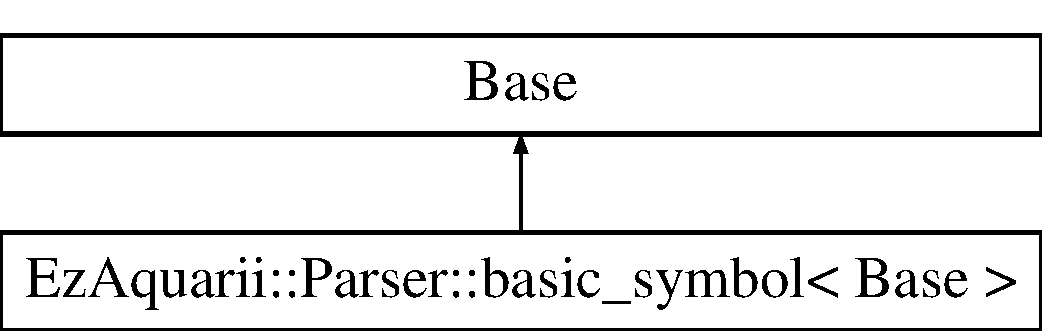
\includegraphics[height=2.000000cm]{structEzAquarii_1_1Parser_1_1basic__symbol}
\end{center}
\end{figure}
\subsection*{Public Types}
\begin{DoxyCompactItemize}
\item 
typedef Base \hyperlink{structEzAquarii_1_1Parser_1_1basic__symbol_aaf4f23168a670058fa38f5aa15d65b75}{super\+\_\+type}\hypertarget{structEzAquarii_1_1Parser_1_1basic__symbol_aaf4f23168a670058fa38f5aa15d65b75}{}\label{structEzAquarii_1_1Parser_1_1basic__symbol_aaf4f23168a670058fa38f5aa15d65b75}

\begin{DoxyCompactList}\small\item\em Alias to Base. \end{DoxyCompactList}\end{DoxyCompactItemize}
\subsection*{Public Member Functions}
\begin{DoxyCompactItemize}
\item 
\hyperlink{structEzAquarii_1_1Parser_1_1basic__symbol_aa5567e1946efcc7e0d083d354d7a9748}{basic\+\_\+symbol} ()\hypertarget{structEzAquarii_1_1Parser_1_1basic__symbol_aa5567e1946efcc7e0d083d354d7a9748}{}\label{structEzAquarii_1_1Parser_1_1basic__symbol_aa5567e1946efcc7e0d083d354d7a9748}

\begin{DoxyCompactList}\small\item\em Default constructor. \end{DoxyCompactList}\item 
\hyperlink{structEzAquarii_1_1Parser_1_1basic__symbol_aae065b3313260ceb34ae03cdb68d2140}{basic\+\_\+symbol} (const \hyperlink{structEzAquarii_1_1Parser_1_1basic__symbol}{basic\+\_\+symbol} \&other)\hypertarget{structEzAquarii_1_1Parser_1_1basic__symbol_aae065b3313260ceb34ae03cdb68d2140}{}\label{structEzAquarii_1_1Parser_1_1basic__symbol_aae065b3313260ceb34ae03cdb68d2140}

\begin{DoxyCompactList}\small\item\em Copy constructor. \end{DoxyCompactList}\item 
\hyperlink{structEzAquarii_1_1Parser_1_1basic__symbol_a09d785a29250b9fbd37d749fc15f5a58}{basic\+\_\+symbol} (typename Base\+::kind\+\_\+type t, const \hyperlink{classEzAquarii_1_1Parser_acc4b937a827f1be285bf28ec90eeb125}{location\+\_\+type} \&l)\hypertarget{structEzAquarii_1_1Parser_1_1basic__symbol_a09d785a29250b9fbd37d749fc15f5a58}{}\label{structEzAquarii_1_1Parser_1_1basic__symbol_a09d785a29250b9fbd37d749fc15f5a58}

\begin{DoxyCompactList}\small\item\em Constructor for valueless symbols, and symbols from each type. \end{DoxyCompactList}\item 
{\bfseries basic\+\_\+symbol} (typename Base\+::kind\+\_\+type t, const class \hyperlink{classCalculationNode}{Calculation\+Node} $\ast$v, const \hyperlink{classEzAquarii_1_1Parser_acc4b937a827f1be285bf28ec90eeb125}{location\+\_\+type} \&l)\hypertarget{structEzAquarii_1_1Parser_1_1basic__symbol_afae6d4626a49350f5765cd498d4d5f27}{}\label{structEzAquarii_1_1Parser_1_1basic__symbol_afae6d4626a49350f5765cd498d4d5f27}

\item 
{\bfseries basic\+\_\+symbol} (typename Base\+::kind\+\_\+type t, const double v, const \hyperlink{classEzAquarii_1_1Parser_acc4b937a827f1be285bf28ec90eeb125}{location\+\_\+type} \&l)\hypertarget{structEzAquarii_1_1Parser_1_1basic__symbol_a38c2d31b6c881387ac382235fd1c46db}{}\label{structEzAquarii_1_1Parser_1_1basic__symbol_a38c2d31b6c881387ac382235fd1c46db}

\item 
{\bfseries basic\+\_\+symbol} (typename Base\+::kind\+\_\+type t, const int v, const \hyperlink{classEzAquarii_1_1Parser_acc4b937a827f1be285bf28ec90eeb125}{location\+\_\+type} \&l)\hypertarget{structEzAquarii_1_1Parser_1_1basic__symbol_a7b39bce7e835ac70a49dbc8747250ce9}{}\label{structEzAquarii_1_1Parser_1_1basic__symbol_a7b39bce7e835ac70a49dbc8747250ce9}

\item 
{\bfseries basic\+\_\+symbol} (typename Base\+::kind\+\_\+type t, const std\+::string v, const \hyperlink{classEzAquarii_1_1Parser_acc4b937a827f1be285bf28ec90eeb125}{location\+\_\+type} \&l)\hypertarget{structEzAquarii_1_1Parser_1_1basic__symbol_a79bff82f60d146ea55733ed85c39071c}{}\label{structEzAquarii_1_1Parser_1_1basic__symbol_a79bff82f60d146ea55733ed85c39071c}

\item 
\hyperlink{structEzAquarii_1_1Parser_1_1basic__symbol_aef39b38d4b4b7fb960becd6d2c488319}{basic\+\_\+symbol} (typename Base\+::kind\+\_\+type t, const \hyperlink{classEzAquarii_1_1Parser_aaaaae6127b81aac6e8be99c12433702e}{semantic\+\_\+type} \&v, const \hyperlink{classEzAquarii_1_1Parser_acc4b937a827f1be285bf28ec90eeb125}{location\+\_\+type} \&l)\hypertarget{structEzAquarii_1_1Parser_1_1basic__symbol_aef39b38d4b4b7fb960becd6d2c488319}{}\label{structEzAquarii_1_1Parser_1_1basic__symbol_aef39b38d4b4b7fb960becd6d2c488319}

\begin{DoxyCompactList}\small\item\em Constructor for symbols with semantic value. \end{DoxyCompactList}\item 
\hyperlink{structEzAquarii_1_1Parser_1_1basic__symbol_a81d711ad681f7aee3cb84e2a9063b4ca}{$\sim$basic\+\_\+symbol} ()\hypertarget{structEzAquarii_1_1Parser_1_1basic__symbol_a81d711ad681f7aee3cb84e2a9063b4ca}{}\label{structEzAquarii_1_1Parser_1_1basic__symbol_a81d711ad681f7aee3cb84e2a9063b4ca}

\begin{DoxyCompactList}\small\item\em Destroy the symbol. \end{DoxyCompactList}\item 
void \hyperlink{structEzAquarii_1_1Parser_1_1basic__symbol_a425715a1798d93c5a35f347af17e993b}{clear} ()\hypertarget{structEzAquarii_1_1Parser_1_1basic__symbol_a425715a1798d93c5a35f347af17e993b}{}\label{structEzAquarii_1_1Parser_1_1basic__symbol_a425715a1798d93c5a35f347af17e993b}

\begin{DoxyCompactList}\small\item\em Destroy contents, and record that is empty. \end{DoxyCompactList}\item 
bool \hyperlink{structEzAquarii_1_1Parser_1_1basic__symbol_a8417f7d2f797554de6cf74ed08436baf}{empty} () const \hypertarget{structEzAquarii_1_1Parser_1_1basic__symbol_a8417f7d2f797554de6cf74ed08436baf}{}\label{structEzAquarii_1_1Parser_1_1basic__symbol_a8417f7d2f797554de6cf74ed08436baf}

\begin{DoxyCompactList}\small\item\em Whether empty. \end{DoxyCompactList}\item 
void \hyperlink{structEzAquarii_1_1Parser_1_1basic__symbol_a72919465bd0c4591aacf01d21ccd1add}{move} (\hyperlink{structEzAquarii_1_1Parser_1_1basic__symbol}{basic\+\_\+symbol} \&s)\hypertarget{structEzAquarii_1_1Parser_1_1basic__symbol_a72919465bd0c4591aacf01d21ccd1add}{}\label{structEzAquarii_1_1Parser_1_1basic__symbol_a72919465bd0c4591aacf01d21ccd1add}

\begin{DoxyCompactList}\small\item\em Destructive move, {\itshape s} is emptied into this. \end{DoxyCompactList}\end{DoxyCompactItemize}
\subsection*{Public Attributes}
\begin{DoxyCompactItemize}
\item 
\hyperlink{classEzAquarii_1_1Parser_aaaaae6127b81aac6e8be99c12433702e}{semantic\+\_\+type} \hyperlink{structEzAquarii_1_1Parser_1_1basic__symbol_ad4222494987bf3e60a3bf224a0ecd4c9}{value}\hypertarget{structEzAquarii_1_1Parser_1_1basic__symbol_ad4222494987bf3e60a3bf224a0ecd4c9}{}\label{structEzAquarii_1_1Parser_1_1basic__symbol_ad4222494987bf3e60a3bf224a0ecd4c9}

\begin{DoxyCompactList}\small\item\em The semantic value. \end{DoxyCompactList}\item 
\hyperlink{classEzAquarii_1_1Parser_acc4b937a827f1be285bf28ec90eeb125}{location\+\_\+type} \hyperlink{structEzAquarii_1_1Parser_1_1basic__symbol_a86d0e10ce513f835e2b442ed297e9ae7}{location}\hypertarget{structEzAquarii_1_1Parser_1_1basic__symbol_a86d0e10ce513f835e2b442ed297e9ae7}{}\label{structEzAquarii_1_1Parser_1_1basic__symbol_a86d0e10ce513f835e2b442ed297e9ae7}

\begin{DoxyCompactList}\small\item\em The location. \end{DoxyCompactList}\end{DoxyCompactItemize}


\subsection{Detailed Description}
\subsubsection*{template$<$typename Base$>$\\*
struct Ez\+Aquarii\+::\+Parser\+::basic\+\_\+symbol$<$ Base $>$}

A complete symbol.

Expects its Base type to provide access to the symbol type via type\+\_\+get().

Provide access to semantic value and location. 

The documentation for this struct was generated from the following file\+:\begin{DoxyCompactItemize}
\item 
/home/mate/\+Documents/\+Programming/\+Research/\+Multilayer\+Network\+Model/\+Multilayer\+Network\+Model/src/parser/include/\hyperlink{parser_8hpp}{parser.\+hpp}\end{DoxyCompactItemize}

\hypertarget{structEzAquarii_1_1Parser_1_1by__type}{}\section{Ez\+Aquarii\+:\+:Parser\+:\+:by\+\_\+type Struct Reference}
\label{structEzAquarii_1_1Parser_1_1by__type}\index{Ez\+Aquarii\+::\+Parser\+::by\+\_\+type@{Ez\+Aquarii\+::\+Parser\+::by\+\_\+type}}


Type access provider for token (enum) based symbols.  




{\ttfamily \#include $<$parser.\+hpp$>$}

\subsection*{Public Types}
\begin{DoxyCompactItemize}
\item 
typedef \hyperlink{classEzAquarii_1_1Parser_a56291d58866809533c2eb3f54911674c}{token\+\_\+type} \hyperlink{structEzAquarii_1_1Parser_1_1by__type_ae6736318831cab4f8b3ab30f414a33e6}{kind\+\_\+type}\hypertarget{structEzAquarii_1_1Parser_1_1by__type_ae6736318831cab4f8b3ab30f414a33e6}{}\label{structEzAquarii_1_1Parser_1_1by__type_ae6736318831cab4f8b3ab30f414a33e6}

\begin{DoxyCompactList}\small\item\em The symbol type as needed by the constructor. \end{DoxyCompactList}\end{DoxyCompactItemize}
\subsection*{Public Member Functions}
\begin{DoxyCompactItemize}
\item 
\hyperlink{structEzAquarii_1_1Parser_1_1by__type_acbd0e48110a4534ec38fe67a6ba53fc1}{by\+\_\+type} ()\hypertarget{structEzAquarii_1_1Parser_1_1by__type_acbd0e48110a4534ec38fe67a6ba53fc1}{}\label{structEzAquarii_1_1Parser_1_1by__type_acbd0e48110a4534ec38fe67a6ba53fc1}

\begin{DoxyCompactList}\small\item\em Default constructor. \end{DoxyCompactList}\item 
\hyperlink{structEzAquarii_1_1Parser_1_1by__type_a825c085d01ea1bf946deb11744befe4c}{by\+\_\+type} (const \hyperlink{structEzAquarii_1_1Parser_1_1by__type}{by\+\_\+type} \&other)\hypertarget{structEzAquarii_1_1Parser_1_1by__type_a825c085d01ea1bf946deb11744befe4c}{}\label{structEzAquarii_1_1Parser_1_1by__type_a825c085d01ea1bf946deb11744befe4c}

\begin{DoxyCompactList}\small\item\em Copy constructor. \end{DoxyCompactList}\item 
\hyperlink{structEzAquarii_1_1Parser_1_1by__type_af78597dca1d15090c5a97243af249f85}{by\+\_\+type} (\hyperlink{structEzAquarii_1_1Parser_1_1by__type_ae6736318831cab4f8b3ab30f414a33e6}{kind\+\_\+type} t)\hypertarget{structEzAquarii_1_1Parser_1_1by__type_af78597dca1d15090c5a97243af249f85}{}\label{structEzAquarii_1_1Parser_1_1by__type_af78597dca1d15090c5a97243af249f85}

\begin{DoxyCompactList}\small\item\em Constructor from (external) token numbers. \end{DoxyCompactList}\item 
void \hyperlink{structEzAquarii_1_1Parser_1_1by__type_aafe02e0cc2a8062eb9ea5fb9f55bf9aa}{clear} ()\hypertarget{structEzAquarii_1_1Parser_1_1by__type_aafe02e0cc2a8062eb9ea5fb9f55bf9aa}{}\label{structEzAquarii_1_1Parser_1_1by__type_aafe02e0cc2a8062eb9ea5fb9f55bf9aa}

\begin{DoxyCompactList}\small\item\em Record that this symbol is empty. \end{DoxyCompactList}\item 
void \hyperlink{structEzAquarii_1_1Parser_1_1by__type_abfbb942b2c579a5c6f43ec1dc9fc91ce}{move} (\hyperlink{structEzAquarii_1_1Parser_1_1by__type}{by\+\_\+type} \&that)\hypertarget{structEzAquarii_1_1Parser_1_1by__type_abfbb942b2c579a5c6f43ec1dc9fc91ce}{}\label{structEzAquarii_1_1Parser_1_1by__type_abfbb942b2c579a5c6f43ec1dc9fc91ce}

\begin{DoxyCompactList}\small\item\em Steal the symbol type from {\itshape that}. \end{DoxyCompactList}\item 
\hyperlink{classEzAquarii_1_1Parser_a6b10da3f2fe3a3c8eaaf290343985935}{symbol\+\_\+number\+\_\+type} \hyperlink{structEzAquarii_1_1Parser_1_1by__type_a8d138a6b3fb230852c22967330ccd44b}{type\+\_\+get} () const 
\item 
\hyperlink{classEzAquarii_1_1Parser_a56291d58866809533c2eb3f54911674c}{token\+\_\+type} \hyperlink{structEzAquarii_1_1Parser_1_1by__type_aa65cdc8218313785870dc6bfed537ca4}{token} () const \hypertarget{structEzAquarii_1_1Parser_1_1by__type_aa65cdc8218313785870dc6bfed537ca4}{}\label{structEzAquarii_1_1Parser_1_1by__type_aa65cdc8218313785870dc6bfed537ca4}

\begin{DoxyCompactList}\small\item\em The token. \end{DoxyCompactList}\end{DoxyCompactItemize}
\subsection*{Public Attributes}
\begin{DoxyCompactItemize}
\item 
int \hyperlink{structEzAquarii_1_1Parser_1_1by__type_ace551e79e70eb0e2237dbab411f478a8}{type}
\end{DoxyCompactItemize}


\subsection{Detailed Description}
Type access provider for token (enum) based symbols. 

\subsection{Member Function Documentation}
\index{Ez\+Aquarii\+::\+Parser\+::by\+\_\+type@{Ez\+Aquarii\+::\+Parser\+::by\+\_\+type}!type\+\_\+get@{type\+\_\+get}}
\index{type\+\_\+get@{type\+\_\+get}!Ez\+Aquarii\+::\+Parser\+::by\+\_\+type@{Ez\+Aquarii\+::\+Parser\+::by\+\_\+type}}
\subsubsection[{\texorpdfstring{type\+\_\+get() const }{type_get() const }}]{\setlength{\rightskip}{0pt plus 5cm}int Ez\+Aquarii\+::\+Parser\+::by\+\_\+type\+::type\+\_\+get (
\begin{DoxyParamCaption}
{}
\end{DoxyParamCaption}
) const\hspace{0.3cm}{\ttfamily [inline]}}\hypertarget{structEzAquarii_1_1Parser_1_1by__type_a8d138a6b3fb230852c22967330ccd44b}{}\label{structEzAquarii_1_1Parser_1_1by__type_a8d138a6b3fb230852c22967330ccd44b}
The (internal) type number (corresponding to {\itshape type}). {\itshape empty} when empty. 

\subsection{Member Data Documentation}
\index{Ez\+Aquarii\+::\+Parser\+::by\+\_\+type@{Ez\+Aquarii\+::\+Parser\+::by\+\_\+type}!type@{type}}
\index{type@{type}!Ez\+Aquarii\+::\+Parser\+::by\+\_\+type@{Ez\+Aquarii\+::\+Parser\+::by\+\_\+type}}
\subsubsection[{\texorpdfstring{type}{type}}]{\setlength{\rightskip}{0pt plus 5cm}int Ez\+Aquarii\+::\+Parser\+::by\+\_\+type\+::type}\hypertarget{structEzAquarii_1_1Parser_1_1by__type_ace551e79e70eb0e2237dbab411f478a8}{}\label{structEzAquarii_1_1Parser_1_1by__type_ace551e79e70eb0e2237dbab411f478a8}
The symbol type. {\itshape empty\+\_\+symbol} when empty. An int, not token\+\_\+number\+\_\+type, to be able to store empty\+\_\+symbol. 

The documentation for this struct was generated from the following file\+:\begin{DoxyCompactItemize}
\item 
/home/mate/\+Documents/\+Programming/\+Research/\+Multilayer\+Network\+Model/\+Multilayer\+Network\+Model/src/parser/include/\hyperlink{parser_8hpp}{parser.\+hpp}\end{DoxyCompactItemize}

\hypertarget{classCalculationNode}{}\section{Calculation\+Node Class Reference}
\label{classCalculationNode}\index{Calculation\+Node@{Calculation\+Node}}
Inheritance diagram for Calculation\+Node\+:\begin{figure}[H]
\begin{center}
\leavevmode
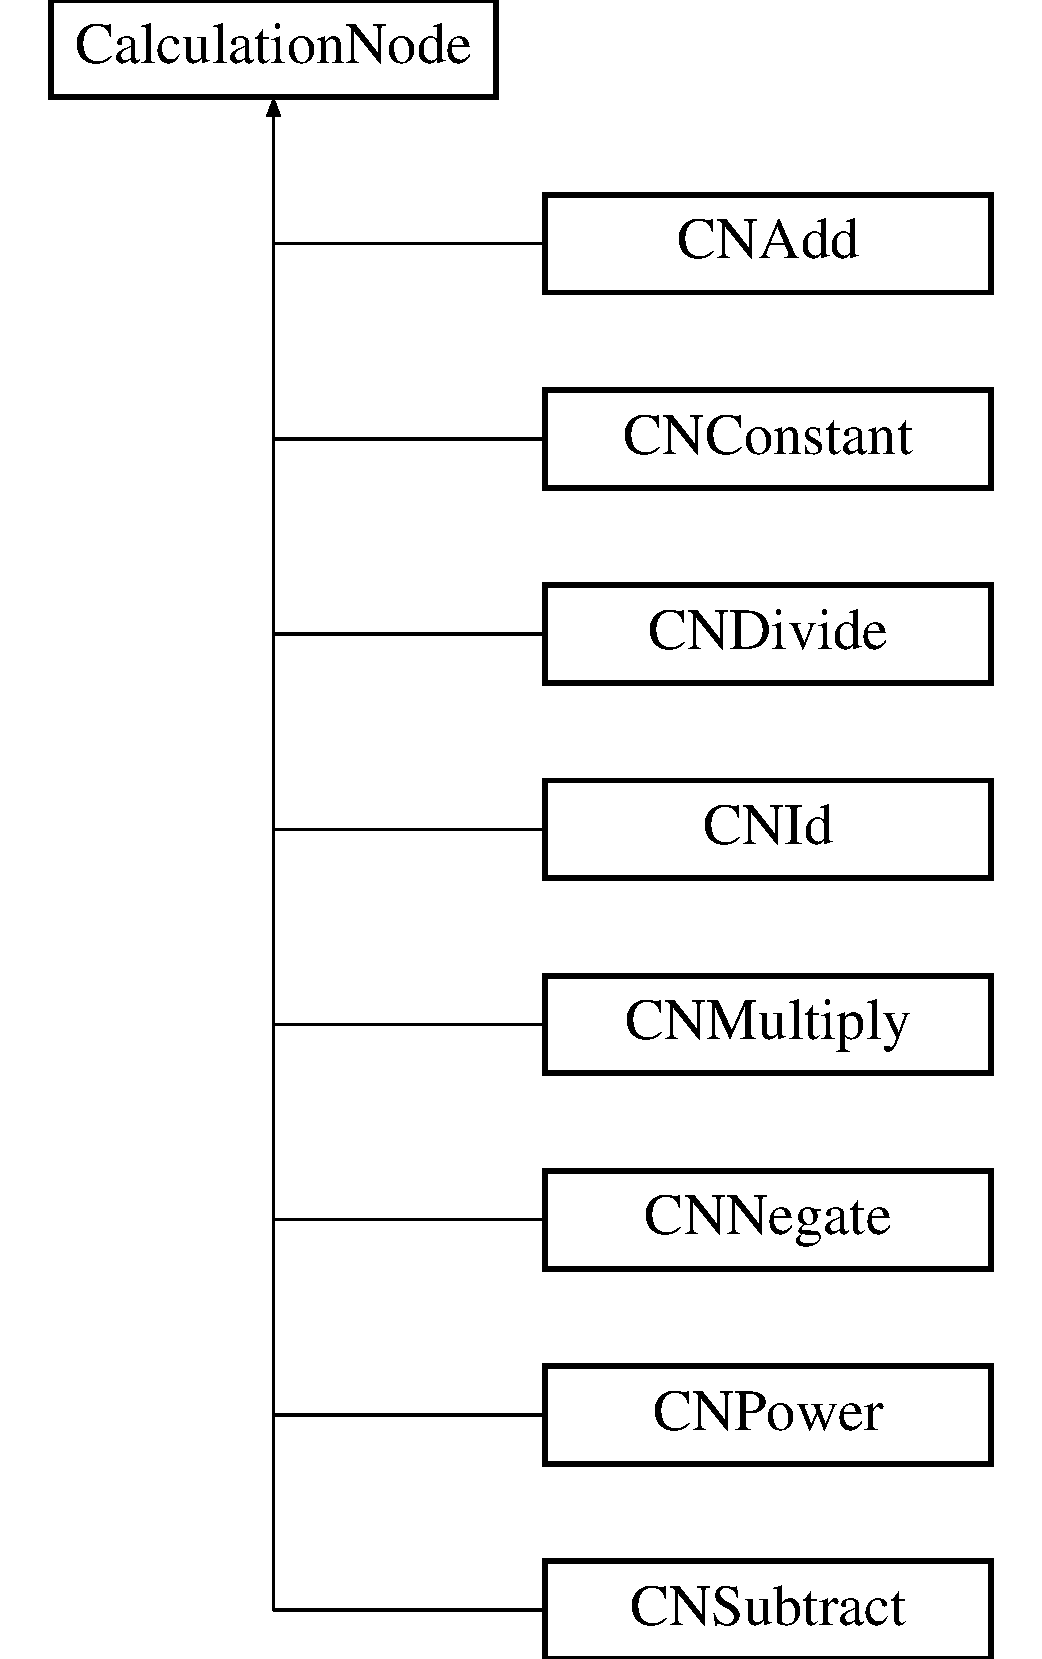
\includegraphics[height=9.000000cm]{classCalculationNode}
\end{center}
\end{figure}
\subsection*{Public Member Functions}
\begin{DoxyCompactItemize}
\item 
virtual double {\bfseries evaluate} () const  =0\hypertarget{classCalculationNode_ac0b4e69fc8bfc99b0ad178b4eeb15883}{}\label{classCalculationNode_ac0b4e69fc8bfc99b0ad178b4eeb15883}

\item 
virtual double {\bfseries evaluate\+At\+State} (std\+::map$<$ int, double $>$) const  =0\hypertarget{classCalculationNode_a15efb576650532bbf21a11f1f9bcb1b2}{}\label{classCalculationNode_a15efb576650532bbf21a11f1f9bcb1b2}

\item 
virtual bool {\bfseries test\+Node\+Ids} () const  =0\hypertarget{classCalculationNode_a4089a2510d7c345a9632843a3fed4f0e}{}\label{classCalculationNode_a4089a2510d7c345a9632843a3fed4f0e}

\item 
virtual std\+::string {\bfseries to\+String} () const  =0\hypertarget{classCalculationNode_aeee8e0d2c7d5c97e0d6801e9644cd686}{}\label{classCalculationNode_aeee8e0d2c7d5c97e0d6801e9644cd686}

\item 
virtual double {\bfseries get\+Value} () const \hypertarget{classCalculationNode_af23ecff57877120eea2f402bb8432549}{}\label{classCalculationNode_af23ecff57877120eea2f402bb8432549}

\item 
virtual void {\bfseries set\+Value} (double value)\hypertarget{classCalculationNode_a63783e44f06e8b665f2f6851616b2965}{}\label{classCalculationNode_a63783e44f06e8b665f2f6851616b2965}

\item 
Calc\+Node\+Types {\bfseries get\+Type} ()\hypertarget{classCalculationNode_ad5df05ec0725d5c4c44b6eecc158a83b}{}\label{classCalculationNode_ad5df05ec0725d5c4c44b6eecc158a83b}

\item 
virtual int {\bfseries get\+Id} ()\hypertarget{classCalculationNode_a57d514437cfc918ddb298d482358c82d}{}\label{classCalculationNode_a57d514437cfc918ddb298d482358c82d}

\item 
virtual void {\bfseries set\+Node} (\hyperlink{classNode}{Node} $\ast$node)\hypertarget{classCalculationNode_a4097a8577ad76d94c32250d76988353c}{}\label{classCalculationNode_a4097a8577ad76d94c32250d76988353c}

\end{DoxyCompactItemize}
\subsection*{Public Attributes}
\begin{DoxyCompactItemize}
\item 
\hyperlink{classCalculationNode}{Calculation\+Node} $\ast$ {\bfseries left}\hypertarget{classCalculationNode_ae82c63d4efc74c0b11a00cc06f225629}{}\label{classCalculationNode_ae82c63d4efc74c0b11a00cc06f225629}

\item 
\hyperlink{classCalculationNode}{Calculation\+Node} $\ast$ {\bfseries right}\hypertarget{classCalculationNode_a55560a0b8fa37b8443c908a06d08f087}{}\label{classCalculationNode_a55560a0b8fa37b8443c908a06d08f087}

\end{DoxyCompactItemize}
\subsection*{Protected Attributes}
\begin{DoxyCompactItemize}
\item 
Calc\+Node\+Types {\bfseries type}\hypertarget{classCalculationNode_a9380df8305abde9a1e3a6a3f5fd6dea0}{}\label{classCalculationNode_a9380df8305abde9a1e3a6a3f5fd6dea0}

\end{DoxyCompactItemize}


The documentation for this class was generated from the following file\+:\begin{DoxyCompactItemize}
\item 
/home/mate/\+Documents/\+Programming/\+Research/\+Multilayer\+Network\+Model/\+Multilayer\+Network\+Model/sources/core/\+Dynamical\+Equation/include/Calculation\+Node.\+hh\end{DoxyCompactItemize}

\hypertarget{classCNAdd}{}\section{C\+N\+Add Class Reference}
\label{classCNAdd}\index{C\+N\+Add@{C\+N\+Add}}
Inheritance diagram for C\+N\+Add\+:\begin{figure}[H]
\begin{center}
\leavevmode
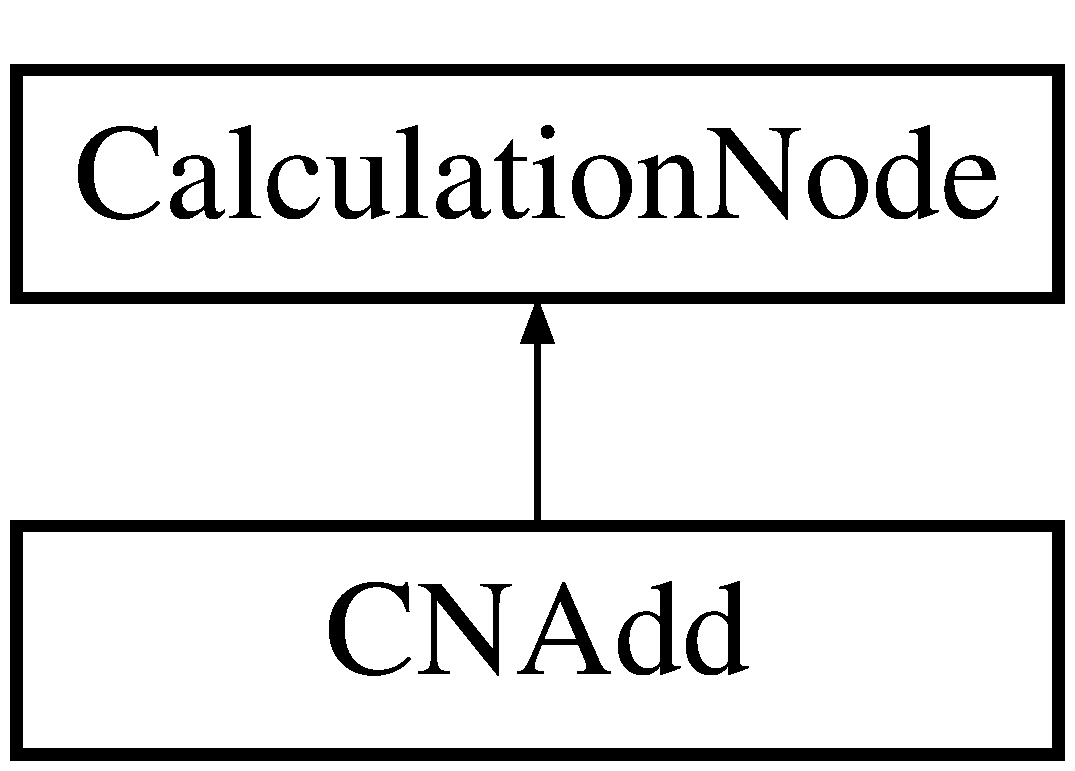
\includegraphics[height=2.000000cm]{classCNAdd}
\end{center}
\end{figure}
\subsection*{Public Member Functions}
\begin{DoxyCompactItemize}
\item 
{\bfseries C\+N\+Add} (\hyperlink{classCalculationNode}{Calculation\+Node} $\ast$\+\_\+left, \hyperlink{classCalculationNode}{Calculation\+Node} $\ast$\+\_\+right)\hypertarget{classCNAdd_a7dab8d6be3e0fa6d804c3593cb1de715}{}\label{classCNAdd_a7dab8d6be3e0fa6d804c3593cb1de715}

\item 
virtual double {\bfseries evaluate} () const \hypertarget{classCNAdd_a5b558f1853ec5555c1ff3503f44b30e7}{}\label{classCNAdd_a5b558f1853ec5555c1ff3503f44b30e7}

\item 
virtual double {\bfseries evaluate\+At\+State} (std\+::map$<$ int, double $>$ starting\+State) const \hypertarget{classCNAdd_a8c4f9b20da9d50fcdd2ac1211da2eee6}{}\label{classCNAdd_a8c4f9b20da9d50fcdd2ac1211da2eee6}

\item 
virtual bool \hyperlink{classCNAdd_a9ded4aa2b5379606d5d110b8cb05ee05}{test\+Node\+Ids} () const 
\item 
virtual std\+::string {\bfseries to\+String} () const \hypertarget{classCNAdd_a6a29c72a161475af0e05361e6cae49cc}{}\label{classCNAdd_a6a29c72a161475af0e05361e6cae49cc}

\end{DoxyCompactItemize}
\subsection*{Additional Inherited Members}


\subsection{Member Function Documentation}
\index{C\+N\+Add@{C\+N\+Add}!test\+Node\+Ids@{test\+Node\+Ids}}
\index{test\+Node\+Ids@{test\+Node\+Ids}!C\+N\+Add@{C\+N\+Add}}
\subsubsection[{\texorpdfstring{test\+Node\+Ids() const }{testNodeIds() const }}]{\setlength{\rightskip}{0pt plus 5cm}virtual bool C\+N\+Add\+::test\+Node\+Ids (
\begin{DoxyParamCaption}
{}
\end{DoxyParamCaption}
) const\hspace{0.3cm}{\ttfamily [inline]}, {\ttfamily [virtual]}}\hypertarget{classCNAdd_a9ded4aa2b5379606d5d110b8cb05ee05}{}\label{classCNAdd_a9ded4aa2b5379606d5d110b8cb05ee05}
Used only for testing puposes. Compared the ID type \hyperlink{classCalculationNode}{Calculation\+Node}\textquotesingle{}s id field to the assigned node\textquotesingle{}s id. 

Implements \hyperlink{classCalculationNode_a4089a2510d7c345a9632843a3fed4f0e}{Calculation\+Node}.



The documentation for this class was generated from the following file\+:\begin{DoxyCompactItemize}
\item 
/home/mate/\+Documents/\+Programming/\+Research/\+Multilayer\+Network\+Model/\+Multilayer\+Network\+Model/sources/core/\+Dynamical\+Equation/include/Calculation\+Node.\+hh\end{DoxyCompactItemize}

\hypertarget{classCNConstant}{}\section{C\+N\+Constant Class Reference}
\label{classCNConstant}\index{C\+N\+Constant@{C\+N\+Constant}}
Inheritance diagram for C\+N\+Constant\+:\begin{figure}[H]
\begin{center}
\leavevmode
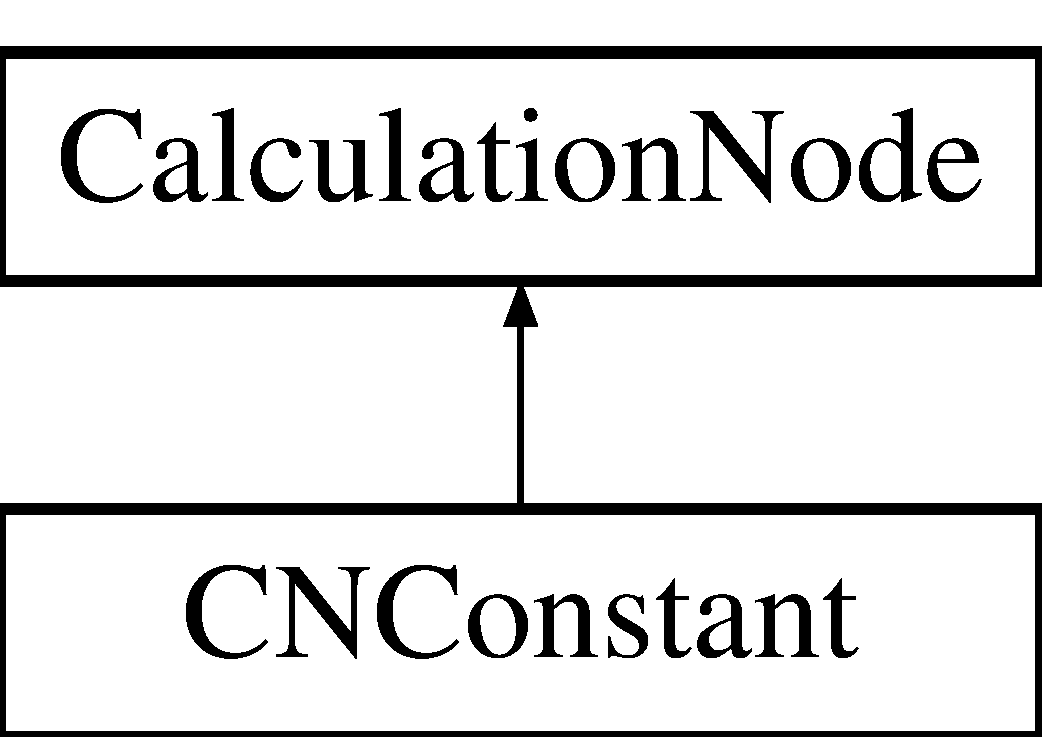
\includegraphics[height=2.000000cm]{classCNConstant}
\end{center}
\end{figure}
\subsection*{Public Member Functions}
\begin{DoxyCompactItemize}
\item 
{\bfseries C\+N\+Constant} (double \+\_\+value)\hypertarget{classCNConstant_a0cf39e7ec935e90a472f8bf4fd784fa2}{}\label{classCNConstant_a0cf39e7ec935e90a472f8bf4fd784fa2}

\item 
virtual double {\bfseries evaluate} () const \hypertarget{classCNConstant_af8f9ed8124c661e1dd31df7e6eed94c3}{}\label{classCNConstant_af8f9ed8124c661e1dd31df7e6eed94c3}

\item 
virtual double {\bfseries evaluate\+At\+State} (std\+::map$<$ int, double $>$ starting\+State) const \hypertarget{classCNConstant_a00d59d4252567658adfc516169645ff5}{}\label{classCNConstant_a00d59d4252567658adfc516169645ff5}

\item 
virtual bool {\bfseries test\+Node\+Ids} () const \hypertarget{classCNConstant_aaa0511d5aa204f30769f2a3a33f78f91}{}\label{classCNConstant_aaa0511d5aa204f30769f2a3a33f78f91}

\item 
virtual std\+::string {\bfseries to\+String} () const \hypertarget{classCNConstant_abd2085b23c5a3502b645068caf53a43f}{}\label{classCNConstant_abd2085b23c5a3502b645068caf53a43f}

\item 
virtual double {\bfseries get\+Value} () const \hypertarget{classCNConstant_ac416282fca8424c0f3d6d65fa2b96f20}{}\label{classCNConstant_ac416282fca8424c0f3d6d65fa2b96f20}

\item 
virtual void {\bfseries set\+Value} (double value)\hypertarget{classCNConstant_a964d75e6934098c33853009a43685a0e}{}\label{classCNConstant_a964d75e6934098c33853009a43685a0e}

\end{DoxyCompactItemize}
\subsection*{Additional Inherited Members}


The documentation for this class was generated from the following file\+:\begin{DoxyCompactItemize}
\item 
/home/mate/\+Documents/\+Programming/\+Research/\+Multilayer\+Network\+Model/\+Multilayer\+Network\+Model/sources/core/\+Dynamical\+Equation/include/Calculation\+Node.\+hh\end{DoxyCompactItemize}

\hypertarget{classCNDivide}{}\section{C\+N\+Divide Class Reference}
\label{classCNDivide}\index{C\+N\+Divide@{C\+N\+Divide}}
Inheritance diagram for C\+N\+Divide\+:\begin{figure}[H]
\begin{center}
\leavevmode
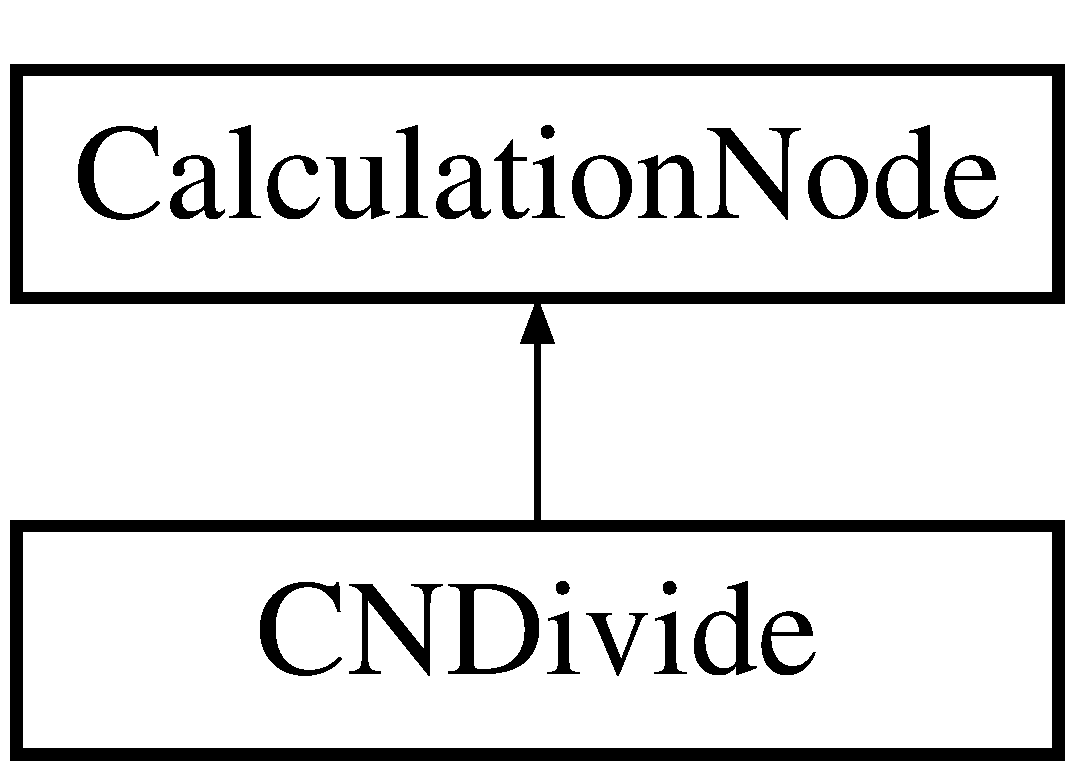
\includegraphics[height=2.000000cm]{classCNDivide}
\end{center}
\end{figure}
\subsection*{Public Member Functions}
\begin{DoxyCompactItemize}
\item 
{\bfseries C\+N\+Divide} (\hyperlink{classCalculationNode}{Calculation\+Node} $\ast$\+\_\+left, \hyperlink{classCalculationNode}{Calculation\+Node} $\ast$\+\_\+right)\hypertarget{classCNDivide_afeb9424f787f42ebf0edb7926a0e80fd}{}\label{classCNDivide_afeb9424f787f42ebf0edb7926a0e80fd}

\item 
virtual double {\bfseries evaluate} () const \hypertarget{classCNDivide_a416c36cec11a481a20bbe3409c1e42db}{}\label{classCNDivide_a416c36cec11a481a20bbe3409c1e42db}

\item 
virtual double {\bfseries evaluate\+At\+State} (std\+::map$<$ int, double $>$ starting\+State) const \hypertarget{classCNDivide_a77752426072bc2bda3b0ca4fdc03f871}{}\label{classCNDivide_a77752426072bc2bda3b0ca4fdc03f871}

\item 
virtual bool {\bfseries test\+Node\+Ids} () const \hypertarget{classCNDivide_a411f954df8b87778f20058ce6601d3f8}{}\label{classCNDivide_a411f954df8b87778f20058ce6601d3f8}

\item 
virtual std\+::string {\bfseries to\+String} () const \hypertarget{classCNDivide_a301fb85c372986362aa6b4930f0d79c5}{}\label{classCNDivide_a301fb85c372986362aa6b4930f0d79c5}

\end{DoxyCompactItemize}
\subsection*{Additional Inherited Members}


The documentation for this class was generated from the following file\+:\begin{DoxyCompactItemize}
\item 
/home/mate/\+Documents/\+Programming/\+Research/\+Multilayer\+Network\+Model/\+Multilayer\+Network\+Model/sources/core/\+Dynamical\+Equation/include/Calculation\+Node.\+hh\end{DoxyCompactItemize}

\hypertarget{classCNId}{}\section{C\+N\+Id Class Reference}
\label{classCNId}\index{C\+N\+Id@{C\+N\+Id}}
Inheritance diagram for C\+N\+Id\+:\begin{figure}[H]
\begin{center}
\leavevmode
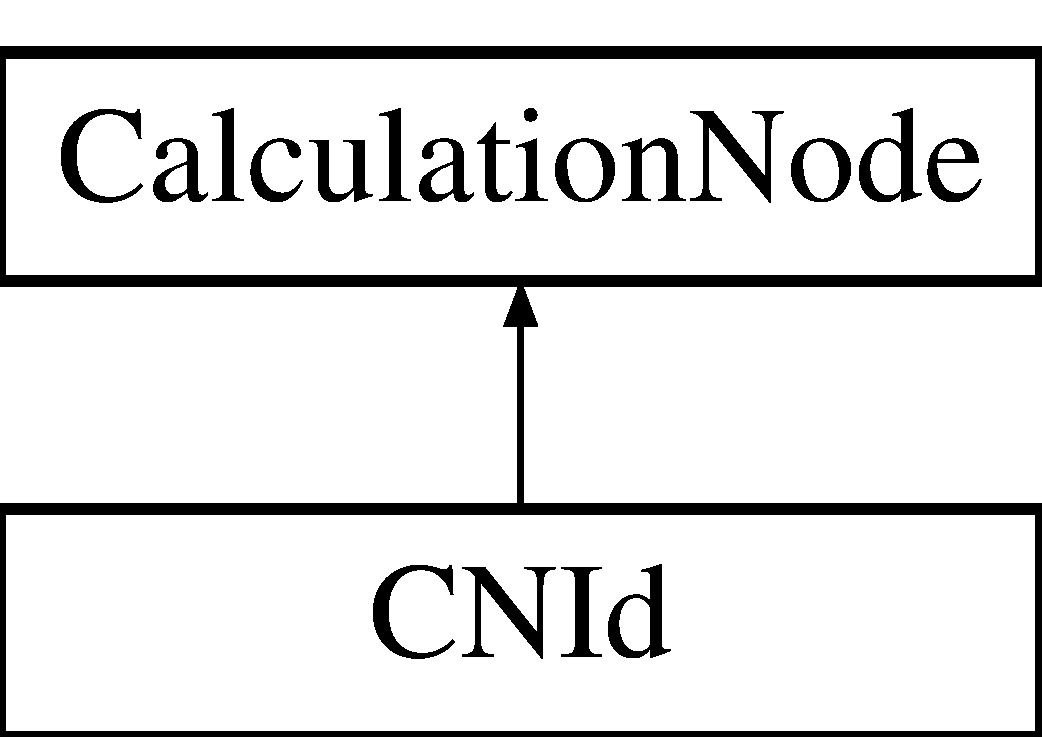
\includegraphics[height=2.000000cm]{classCNId}
\end{center}
\end{figure}
\subsection*{Public Member Functions}
\begin{DoxyCompactItemize}
\item 
{\bfseries C\+N\+Id} (int \+\_\+id)\hypertarget{classCNId_ad36125d5115c0c75783a23e1e4ad55b2}{}\label{classCNId_ad36125d5115c0c75783a23e1e4ad55b2}

\item 
int {\bfseries get\+Id} ()\hypertarget{classCNId_ae0c2d402de892ef8783e6f5281ece008}{}\label{classCNId_ae0c2d402de892ef8783e6f5281ece008}

\item 
void {\bfseries set\+Node} (\hyperlink{classNode}{Node} $\ast$node)\hypertarget{classCNId_a25b7d25adf35e61b0d1b0e67862354f4}{}\label{classCNId_a25b7d25adf35e61b0d1b0e67862354f4}

\item 
virtual double {\bfseries evaluate} () const \hypertarget{classCNId_a5f6b3bbc1a6daaef9a11cdc80aff920c}{}\label{classCNId_a5f6b3bbc1a6daaef9a11cdc80aff920c}

\item 
virtual double {\bfseries evaluate\+At\+State} (std\+::map$<$ int, double $>$ starting\+State) const \hypertarget{classCNId_aacf48e3e3766cc1d54a9af8532d747ec}{}\label{classCNId_aacf48e3e3766cc1d54a9af8532d747ec}

\item 
virtual bool {\bfseries test\+Node\+Ids} () const \hypertarget{classCNId_a0bc1a04e94dfbb047ad53dd6682bf071}{}\label{classCNId_a0bc1a04e94dfbb047ad53dd6682bf071}

\item 
virtual std\+::string {\bfseries to\+String} () const \hypertarget{classCNId_ae853b898d20c008bdddf799ed971f30a}{}\label{classCNId_ae853b898d20c008bdddf799ed971f30a}

\end{DoxyCompactItemize}
\subsection*{Additional Inherited Members}


The documentation for this class was generated from the following files\+:\begin{DoxyCompactItemize}
\item 
/home/mate/\+Documents/\+Programming/\+Research/\+Multilayer\+Network\+Model/\+Multilayer\+Network\+Model/sources/core/\+Dynamical\+Equation/include/Calculation\+Node.\+hh\item 
/home/mate/\+Documents/\+Programming/\+Research/\+Multilayer\+Network\+Model/\+Multilayer\+Network\+Model/sources/core/\+Dynamical\+Equation/src/Calculation\+Node.\+cc\end{DoxyCompactItemize}

\hypertarget{classCNMultiply}{}\section{C\+N\+Multiply Class Reference}
\label{classCNMultiply}\index{C\+N\+Multiply@{C\+N\+Multiply}}
Inheritance diagram for C\+N\+Multiply\+:\begin{figure}[H]
\begin{center}
\leavevmode
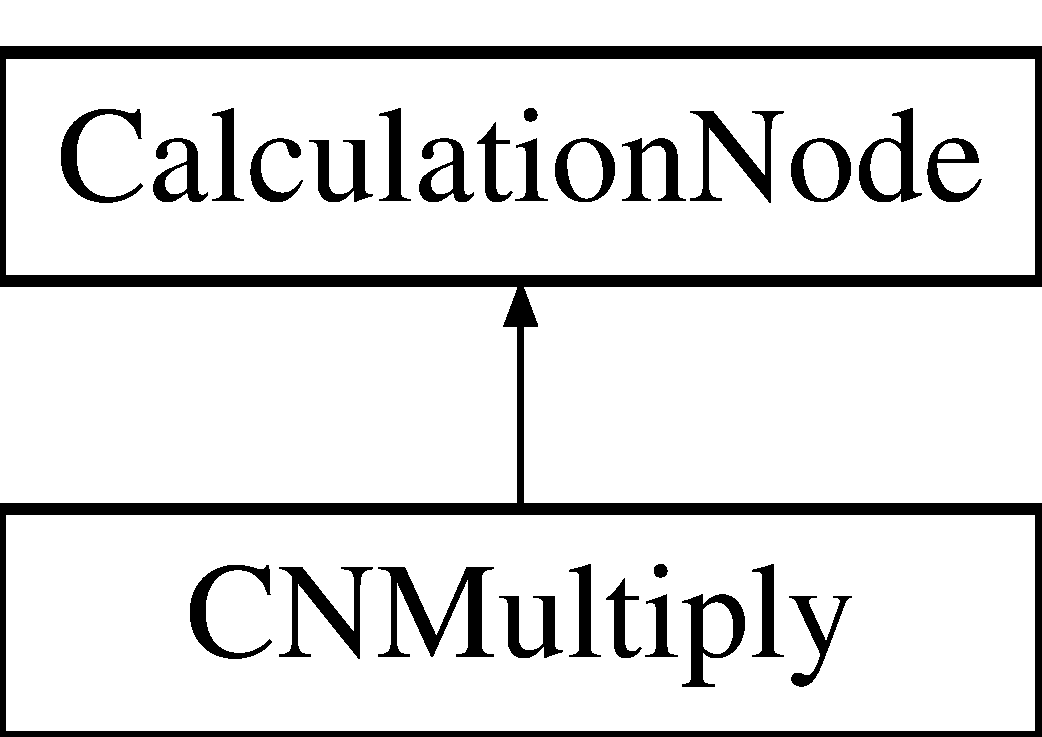
\includegraphics[height=2.000000cm]{classCNMultiply}
\end{center}
\end{figure}
\subsection*{Public Member Functions}
\begin{DoxyCompactItemize}
\item 
{\bfseries C\+N\+Multiply} (\hyperlink{classCalculationNode}{Calculation\+Node} $\ast$\+\_\+left, \hyperlink{classCalculationNode}{Calculation\+Node} $\ast$\+\_\+right)\hypertarget{classCNMultiply_a440c0e25b1fb642c95757a9118634874}{}\label{classCNMultiply_a440c0e25b1fb642c95757a9118634874}

\item 
virtual double {\bfseries evaluate} () const \hypertarget{classCNMultiply_a51ce205165bfa5842002721332c14f5c}{}\label{classCNMultiply_a51ce205165bfa5842002721332c14f5c}

\item 
virtual double {\bfseries evaluate\+At\+State} (std\+::map$<$ int, double $>$ starting\+State) const \hypertarget{classCNMultiply_a8daa0d3ea8f08db43b6e168f6ca9527b}{}\label{classCNMultiply_a8daa0d3ea8f08db43b6e168f6ca9527b}

\item 
virtual bool {\bfseries test\+Node\+Ids} () const \hypertarget{classCNMultiply_a9ffc252a3cc6ccdb3ef9ee4700f0ac18}{}\label{classCNMultiply_a9ffc252a3cc6ccdb3ef9ee4700f0ac18}

\item 
virtual std\+::string {\bfseries to\+String} () const \hypertarget{classCNMultiply_a55edebadef3ea3df839dd8779f1e2e13}{}\label{classCNMultiply_a55edebadef3ea3df839dd8779f1e2e13}

\end{DoxyCompactItemize}
\subsection*{Additional Inherited Members}


The documentation for this class was generated from the following file\+:\begin{DoxyCompactItemize}
\item 
/home/mate/\+Documents/\+Programming/\+Research/\+Multilayer\+Network\+Model/\+Multilayer\+Network\+Model/sources/core/\+Dynamical\+Equation/include/Calculation\+Node.\+hh\end{DoxyCompactItemize}

\hypertarget{classCNNegate}{}\section{C\+N\+Negate Class Reference}
\label{classCNNegate}\index{C\+N\+Negate@{C\+N\+Negate}}
Inheritance diagram for C\+N\+Negate\+:\begin{figure}[H]
\begin{center}
\leavevmode
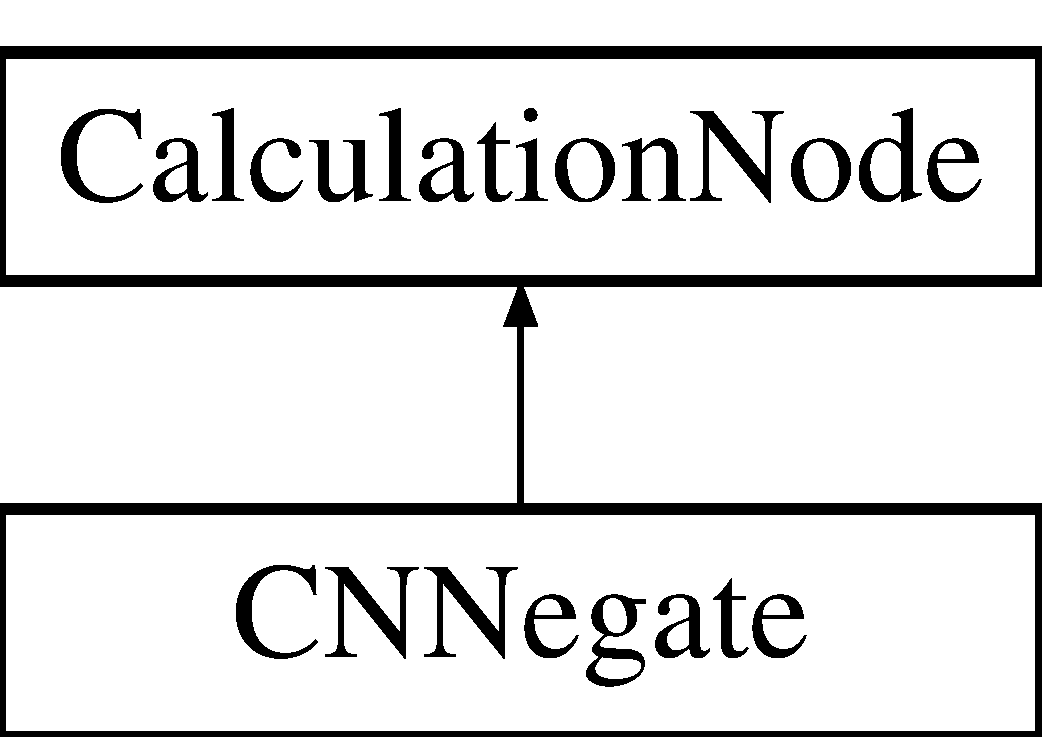
\includegraphics[height=2.000000cm]{classCNNegate}
\end{center}
\end{figure}
\subsection*{Public Member Functions}
\begin{DoxyCompactItemize}
\item 
{\bfseries C\+N\+Negate} (\hyperlink{classCalculationNode}{Calculation\+Node} $\ast$\+\_\+right)\hypertarget{classCNNegate_a7ed8699cfcdf9e6cb4e08c2f386ec8aa}{}\label{classCNNegate_a7ed8699cfcdf9e6cb4e08c2f386ec8aa}

\item 
virtual double {\bfseries evaluate} () const \hypertarget{classCNNegate_ad8742ef807da75fea0d512467d5331cd}{}\label{classCNNegate_ad8742ef807da75fea0d512467d5331cd}

\item 
virtual double {\bfseries evaluate\+At\+State} (std\+::map$<$ int, double $>$ starting\+State) const \hypertarget{classCNNegate_a466eaeee589ea62f77dab230b4da9ab7}{}\label{classCNNegate_a466eaeee589ea62f77dab230b4da9ab7}

\item 
virtual bool {\bfseries test\+Node\+Ids} () const \hypertarget{classCNNegate_ad03475bf5217a1673057e74f60b7b7fe}{}\label{classCNNegate_ad03475bf5217a1673057e74f60b7b7fe}

\item 
virtual std\+::string {\bfseries to\+String} () const \hypertarget{classCNNegate_a8cf6b243b14cfbeb28434f301303d1a9}{}\label{classCNNegate_a8cf6b243b14cfbeb28434f301303d1a9}

\end{DoxyCompactItemize}
\subsection*{Additional Inherited Members}


The documentation for this class was generated from the following file\+:\begin{DoxyCompactItemize}
\item 
/home/mate/\+Documents/\+Programming/\+Research/\+Multilayer\+Network\+Model/\+Multilayer\+Network\+Model/sources/core/\+Dynamical\+Equation/include/Calculation\+Node.\+hh\end{DoxyCompactItemize}

\hypertarget{classCNPower}{}\section{C\+N\+Power Class Reference}
\label{classCNPower}\index{C\+N\+Power@{C\+N\+Power}}
Inheritance diagram for C\+N\+Power\+:\begin{figure}[H]
\begin{center}
\leavevmode
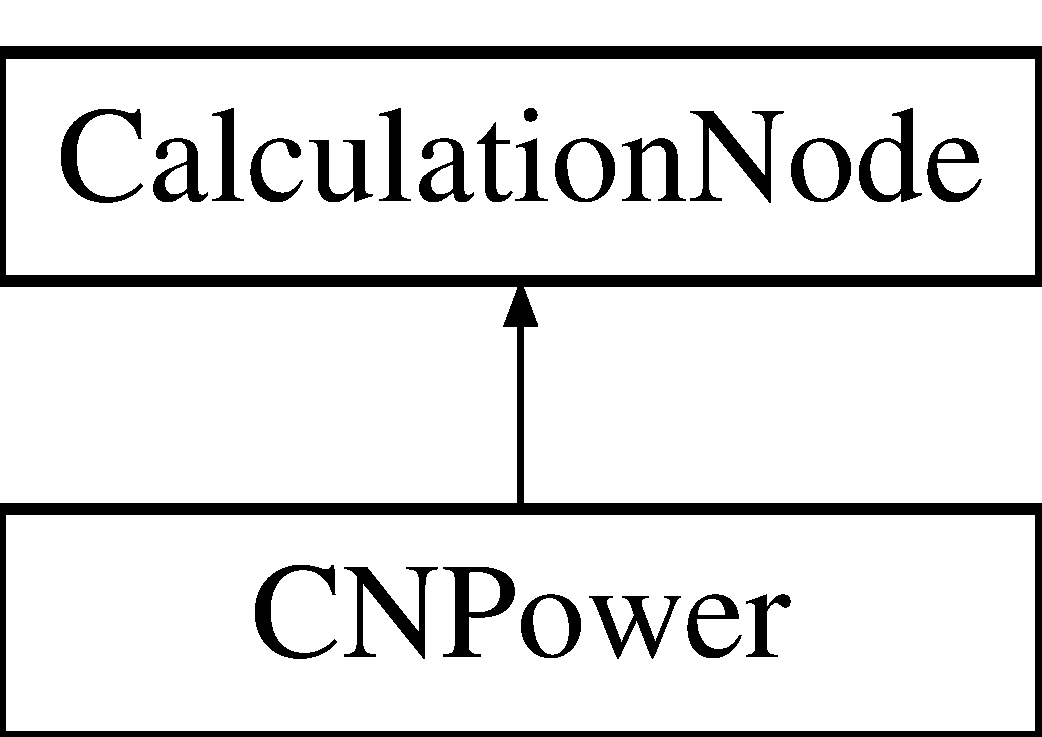
\includegraphics[height=2.000000cm]{classCNPower}
\end{center}
\end{figure}
\subsection*{Public Member Functions}
\begin{DoxyCompactItemize}
\item 
{\bfseries C\+N\+Power} (\hyperlink{classCalculationNode}{Calculation\+Node} $\ast$\+\_\+left, \hyperlink{classCalculationNode}{Calculation\+Node} $\ast$\+\_\+right)\hypertarget{classCNPower_ac5ba8a91170451bc06afbf7153d7f707}{}\label{classCNPower_ac5ba8a91170451bc06afbf7153d7f707}

\item 
virtual double {\bfseries evaluate} () const \hypertarget{classCNPower_a9461646cf8e9fc0cb54318e04d73ed72}{}\label{classCNPower_a9461646cf8e9fc0cb54318e04d73ed72}

\item 
virtual double {\bfseries evaluate\+At\+State} (std\+::map$<$ int, double $>$ starting\+State) const \hypertarget{classCNPower_af4a31cbe51bc44fba203bda91d46384f}{}\label{classCNPower_af4a31cbe51bc44fba203bda91d46384f}

\item 
virtual bool {\bfseries test\+Node\+Ids} () const \hypertarget{classCNPower_a3d1e004e5e71954037b2ea46f54cd438}{}\label{classCNPower_a3d1e004e5e71954037b2ea46f54cd438}

\item 
virtual std\+::string {\bfseries to\+String} () const \hypertarget{classCNPower_a5d9c427cba2ea13f2bf91ecadcac50ef}{}\label{classCNPower_a5d9c427cba2ea13f2bf91ecadcac50ef}

\end{DoxyCompactItemize}
\subsection*{Additional Inherited Members}


The documentation for this class was generated from the following file\+:\begin{DoxyCompactItemize}
\item 
/home/mate/\+Documents/\+Programming/\+Research/\+Multilayer\+Network\+Model/\+Multilayer\+Network\+Model/src/core/include/Calculation\+Node.\+hh\end{DoxyCompactItemize}

\hypertarget{classCNSubtract}{}\section{C\+N\+Subtract Class Reference}
\label{classCNSubtract}\index{C\+N\+Subtract@{C\+N\+Subtract}}
Inheritance diagram for C\+N\+Subtract\+:\begin{figure}[H]
\begin{center}
\leavevmode
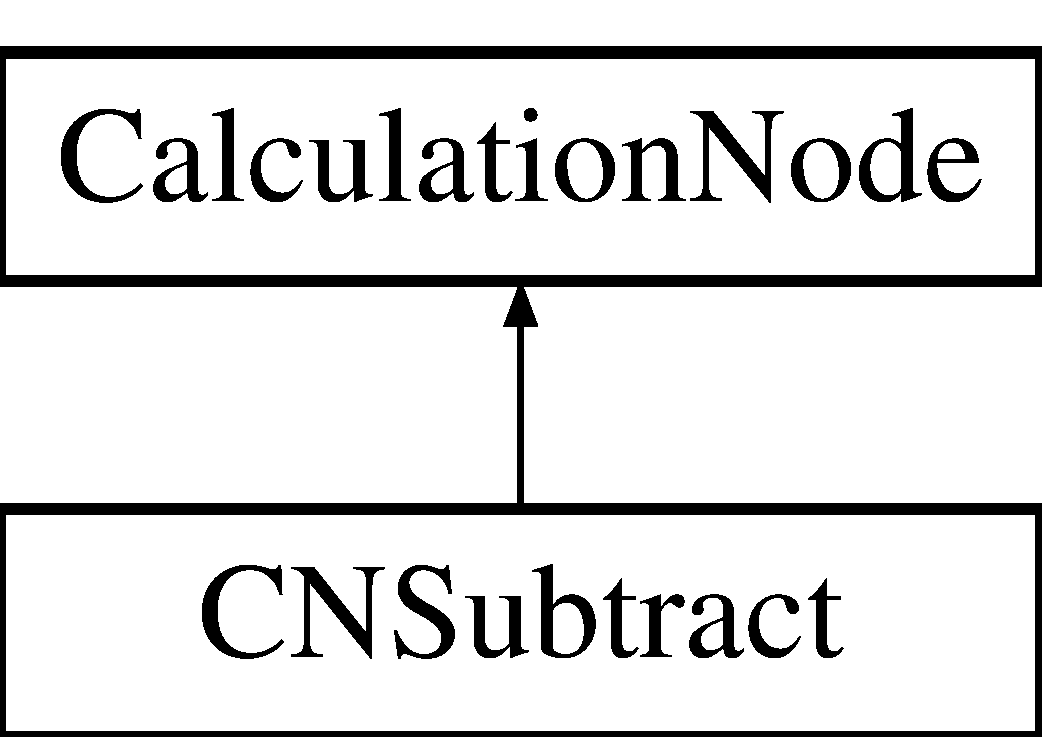
\includegraphics[height=2.000000cm]{classCNSubtract}
\end{center}
\end{figure}
\subsection*{Public Member Functions}
\begin{DoxyCompactItemize}
\item 
{\bfseries C\+N\+Subtract} (\hyperlink{classCalculationNode}{Calculation\+Node} $\ast$\+\_\+left, \hyperlink{classCalculationNode}{Calculation\+Node} $\ast$\+\_\+right)\hypertarget{classCNSubtract_ab72c2b6679137655582d2001ac420dbf}{}\label{classCNSubtract_ab72c2b6679137655582d2001ac420dbf}

\item 
virtual double {\bfseries evaluate} () const \hypertarget{classCNSubtract_ae57879411a77bf2a5b16f28aa488a3d6}{}\label{classCNSubtract_ae57879411a77bf2a5b16f28aa488a3d6}

\item 
virtual double {\bfseries evaluate\+At\+State} (std\+::map$<$ int, double $>$ starting\+State) const \hypertarget{classCNSubtract_aa1d22fea2c4d0cdd26e64725d2be5205}{}\label{classCNSubtract_aa1d22fea2c4d0cdd26e64725d2be5205}

\item 
virtual bool \hyperlink{classCNSubtract_a83d03d12f8b0b209c78dda0d783453e1}{test\+Node\+Ids} () const 
\item 
virtual std\+::string {\bfseries to\+String} () const \hypertarget{classCNSubtract_a19ed00fcb52d52d40d97ed79a62e6dcd}{}\label{classCNSubtract_a19ed00fcb52d52d40d97ed79a62e6dcd}

\end{DoxyCompactItemize}
\subsection*{Additional Inherited Members}


\subsection{Member Function Documentation}
\index{C\+N\+Subtract@{C\+N\+Subtract}!test\+Node\+Ids@{test\+Node\+Ids}}
\index{test\+Node\+Ids@{test\+Node\+Ids}!C\+N\+Subtract@{C\+N\+Subtract}}
\subsubsection[{\texorpdfstring{test\+Node\+Ids() const }{testNodeIds() const }}]{\setlength{\rightskip}{0pt plus 5cm}virtual bool C\+N\+Subtract\+::test\+Node\+Ids (
\begin{DoxyParamCaption}
{}
\end{DoxyParamCaption}
) const\hspace{0.3cm}{\ttfamily [inline]}, {\ttfamily [virtual]}}\hypertarget{classCNSubtract_a83d03d12f8b0b209c78dda0d783453e1}{}\label{classCNSubtract_a83d03d12f8b0b209c78dda0d783453e1}
Used only for testing puposes. Compared the ID type \hyperlink{classCalculationNode}{Calculation\+Node}\textquotesingle{}s id field to the assigned node\textquotesingle{}s id. 

Implements \hyperlink{classCalculationNode_a4089a2510d7c345a9632843a3fed4f0e}{Calculation\+Node}.



The documentation for this class was generated from the following file\+:\begin{DoxyCompactItemize}
\item 
/home/mate/\+Documents/\+Programming/\+Research/\+Multilayer\+Network\+Model/\+Multilayer\+Network\+Model/sources/core/\+Dynamical\+Equation/include/Calculation\+Node.\+hh\end{DoxyCompactItemize}

\hypertarget{classDownwardInfluenceImpl}{}\section{Downward\+Influence\+Impl Class Reference}
\label{classDownwardInfluenceImpl}\index{Downward\+Influence\+Impl@{Downward\+Influence\+Impl}}
Inheritance diagram for Downward\+Influence\+Impl\+:\begin{figure}[H]
\begin{center}
\leavevmode
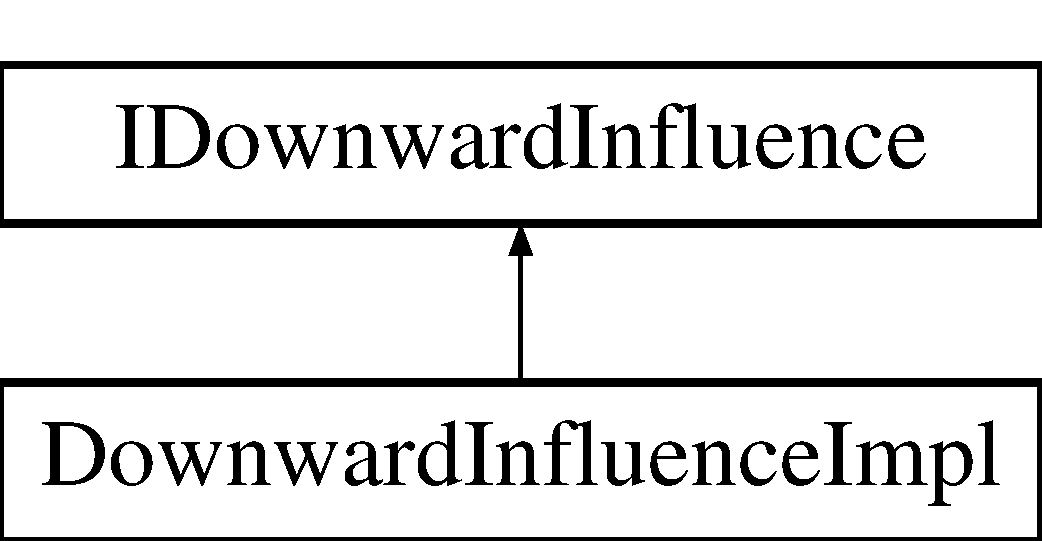
\includegraphics[height=2.000000cm]{classDownwardInfluenceImpl}
\end{center}
\end{figure}
\subsection*{Public Member Functions}
\begin{DoxyCompactItemize}
\item 
{\bfseries Downward\+Influence\+Impl} (\hyperlink{classNode}{Node} $\ast$node)\hypertarget{classDownwardInfluenceImpl_add04549a8e99e67304c133b4d9a46fc9}{}\label{classDownwardInfluenceImpl_add04549a8e99e67304c133b4d9a46fc9}

\item 
void {\bfseries calculate\+Downward\+Influence} ()\hypertarget{classDownwardInfluenceImpl_a05fdd6c5ef32911d503d9262e9431812}{}\label{classDownwardInfluenceImpl_a05fdd6c5ef32911d503d9262e9431812}

\end{DoxyCompactItemize}
\subsection*{Additional Inherited Members}


The documentation for this class was generated from the following files\+:\begin{DoxyCompactItemize}
\item 
/home/mate/\+Documents/\+Programming/\+Research/\+Multilayer\+Network\+Model/\+Multilayer\+Network\+Model/sources/core/\+Downward\+Influence/include/Downward\+Influence\+Impl.\+hh\item 
/home/mate/\+Documents/\+Programming/\+Research/\+Multilayer\+Network\+Model/\+Multilayer\+Network\+Model/sources/core/\+Downward\+Influence/src/Downward\+Influence\+Impl.\+cc\end{DoxyCompactItemize}

\hypertarget{classDynamicalEquation}{}\section{Dynamical\+Equation Class Reference}
\label{classDynamicalEquation}\index{Dynamical\+Equation@{Dynamical\+Equation}}
\subsection*{Public Member Functions}
\begin{DoxyCompactItemize}
\item 
double {\bfseries evaluate} ()\hypertarget{classDynamicalEquation_ac353d833e23a7718d28b48b96f273100}{}\label{classDynamicalEquation_ac353d833e23a7718d28b48b96f273100}

\item 
double {\bfseries evaluate\+At\+State} (std\+::map$<$ int, double $>$ starting\+State)\hypertarget{classDynamicalEquation_adf9454ebe570a95e2b4d72c04bdc82cc}{}\label{classDynamicalEquation_adf9454ebe570a95e2b4d72c04bdc82cc}

\item 
void {\bfseries O\+D\+Ecalculator} (const state\+\_\+type \&x, state\+\_\+type \&dxdt, double t)\hypertarget{classDynamicalEquation_a153f3c990807c596142b45d9f63ab57c}{}\label{classDynamicalEquation_a153f3c990807c596142b45d9f63ab57c}

\item 
void {\bfseries O\+D\+Ecalculator\+At\+State} (const state\+\_\+type \&x, state\+\_\+type \&dxdt, double t, std\+::map$<$ int, double $>$ starting\+State)\hypertarget{classDynamicalEquation_a07a6f24e0ca820c3734545c7d5d65927}{}\label{classDynamicalEquation_a07a6f24e0ca820c3734545c7d5d65927}

\item 
bool {\bfseries test\+Node\+Ids} (void) const \hypertarget{classDynamicalEquation_adbf7e8bad4b2764922b0ba2fe077b297}{}\label{classDynamicalEquation_adbf7e8bad4b2764922b0ba2fe077b297}

\item 
\hyperlink{classCalculationNode}{Calculation\+Node} $\ast$ {\bfseries get\+Base\+Calculation\+Node} (void)\hypertarget{classDynamicalEquation_aaa39d24b8dff72907638441db262c127}{}\label{classDynamicalEquation_aaa39d24b8dff72907638441db262c127}

\item 
void {\bfseries set\+Base\+Calculation\+Node} (\hyperlink{classCalculationNode}{Calculation\+Node} $\ast$base\+Calc\+Node)\hypertarget{classDynamicalEquation_a62f51fc853ccfa0aa2a09c3f2385eebe}{}\label{classDynamicalEquation_a62f51fc853ccfa0aa2a09c3f2385eebe}

\item 
void {\bfseries load\+Equation} (std\+::string str\+Equation)\hypertarget{classDynamicalEquation_aabe35a0aca2762081bd3b880f1648a87}{}\label{classDynamicalEquation_aabe35a0aca2762081bd3b880f1648a87}

\item 
void {\bfseries load\+Nodes\+To\+Equation} (\hyperlink{classCalculationNode}{Calculation\+Node} $\ast$calc\+Ptr, std\+::map$<$ int, \hyperlink{classNode}{Node} $\ast$ $>$ \&nodes\+Map)\hypertarget{classDynamicalEquation_a2c54698f5a05199a87ff0650836ff95c}{}\label{classDynamicalEquation_a2c54698f5a05199a87ff0650836ff95c}

\item 
std\+::string {\bfseries to\+String} () const \hypertarget{classDynamicalEquation_aed67e4c29392eb9c616b64acaa7500bc}{}\label{classDynamicalEquation_aed67e4c29392eb9c616b64acaa7500bc}

\end{DoxyCompactItemize}


The documentation for this class was generated from the following files\+:\begin{DoxyCompactItemize}
\item 
/home/mate/\+Documents/\+Programming/\+Research/\+Multilayer\+Network\+Model/\+Multilayer\+Network\+Model/src/core/include/Dynamical\+Equation.\+hh\item 
/home/mate/\+Documents/\+Programming/\+Research/\+Multilayer\+Network\+Model/\+Multilayer\+Network\+Model/src/core/src/Dynamical\+Equation.\+cc\end{DoxyCompactItemize}

\hypertarget{classDynamicalEquationGeneratorSimpleImpl}{}\section{Dynamical\+Equation\+Generator\+Simple\+Impl Class Reference}
\label{classDynamicalEquationGeneratorSimpleImpl}\index{Dynamical\+Equation\+Generator\+Simple\+Impl@{Dynamical\+Equation\+Generator\+Simple\+Impl}}
Inheritance diagram for Dynamical\+Equation\+Generator\+Simple\+Impl\+:\begin{figure}[H]
\begin{center}
\leavevmode
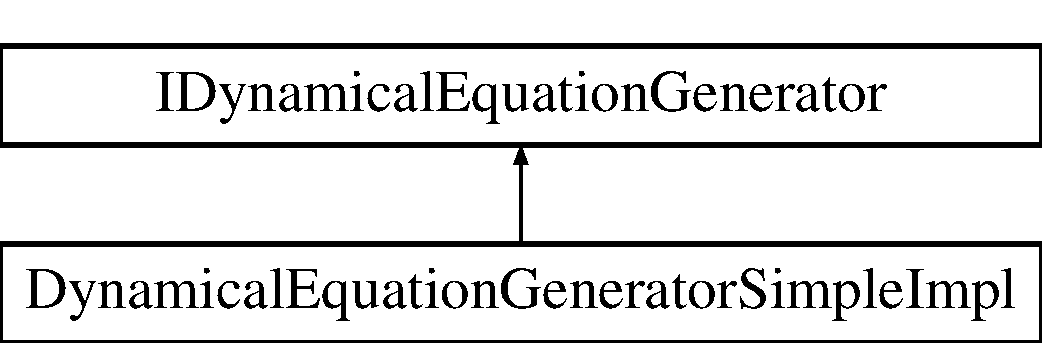
\includegraphics[height=2.000000cm]{classDynamicalEquationGeneratorSimpleImpl}
\end{center}
\end{figure}
\subsection*{Public Member Functions}
\begin{DoxyCompactItemize}
\item 
{\bfseries Dynamical\+Equation\+Generator\+Simple\+Impl} (\hyperlink{classMultilayerNetwork}{Multilayer\+Network} $\ast$multilayer\+Network)\hypertarget{classDynamicalEquationGeneratorSimpleImpl_aefe26119d2db680f1a03fc0b5415474e}{}\label{classDynamicalEquationGeneratorSimpleImpl_aefe26119d2db680f1a03fc0b5415474e}

\item 
void {\bfseries generate\+Dynamical\+Equations} ()\hypertarget{classDynamicalEquationGeneratorSimpleImpl_a92e9bade614a29d3c5351d89d43e98f1}{}\label{classDynamicalEquationGeneratorSimpleImpl_a92e9bade614a29d3c5351d89d43e98f1}

\end{DoxyCompactItemize}
\subsection*{Additional Inherited Members}


The documentation for this class was generated from the following files\+:\begin{DoxyCompactItemize}
\item 
/home/mate/\+Documents/\+Programming/\+Research/\+Multilayer\+Network\+Model/\+Multilayer\+Network\+Model/sources/generators/include/Dynamical\+Equation\+Generator\+Simple\+Impl.\+hh\item 
/home/mate/\+Documents/\+Programming/\+Research/\+Multilayer\+Network\+Model/\+Multilayer\+Network\+Model/sources/generators/src/Dynamical\+Equation\+Generator\+Simple\+Impl.\+cc\end{DoxyCompactItemize}

\hypertarget{classGeneticAlgorithmController}{}\section{Genetic\+Algorithm\+Controller Class Reference}
\label{classGeneticAlgorithmController}\index{Genetic\+Algorithm\+Controller@{Genetic\+Algorithm\+Controller}}
\subsection*{Public Member Functions}
\begin{DoxyCompactItemize}
\item 
void {\bfseries fit\+To\+Vector\+Field} (\hyperlink{classNetwork}{Network} $\ast$network, \hyperlink{classVectorField}{Vector\+Field} $\ast$target\+Vector\+Field)\hypertarget{classGeneticAlgorithmController_a85887ad28acae9e6f01ed15a5eb8485d}{}\label{classGeneticAlgorithmController_a85887ad28acae9e6f01ed15a5eb8485d}

\item 
void {\bfseries mutation} ()\hypertarget{classGeneticAlgorithmController_aeb407ce174447ffd7ef2041af727e23d}{}\label{classGeneticAlgorithmController_aeb407ce174447ffd7ef2041af727e23d}

\item 
void {\bfseries crossover} ()\hypertarget{classGeneticAlgorithmController_aaa7228fb8a37d5b1745c4854d4aa5d46}{}\label{classGeneticAlgorithmController_aaa7228fb8a37d5b1745c4854d4aa5d46}

\item 
void {\bfseries death} ()\hypertarget{classGeneticAlgorithmController_a7586971212107be4213a0151e347a069}{}\label{classGeneticAlgorithmController_a7586971212107be4213a0151e347a069}

\item 
void {\bfseries create\+Initial\+Population} (\hyperlink{classNetwork}{Network} $\ast$network)\hypertarget{classGeneticAlgorithmController_a25892138421bc984d1e7bc069d42b276}{}\label{classGeneticAlgorithmController_a25892138421bc984d1e7bc069d42b276}

\item 
\hyperlink{classNetworkPopulationElement}{Network\+Population\+Element} $\ast$ {\bfseries choose\+For\+Mutation} ()\hypertarget{classGeneticAlgorithmController_a467ce68b08437543a6ccdd8bfc04a0aa}{}\label{classGeneticAlgorithmController_a467ce68b08437543a6ccdd8bfc04a0aa}

\item 
\hyperlink{classNetworkPopulationElement}{Network\+Population\+Element} $\ast$ {\bfseries choose\+For\+Crossover} ()\hypertarget{classGeneticAlgorithmController_ab7e07c9d2cc53fa1964d11b2f6a6294a}{}\label{classGeneticAlgorithmController_ab7e07c9d2cc53fa1964d11b2f6a6294a}

\item 
\hyperlink{classNetworkPopulationElement}{Network\+Population\+Element} $\ast$ {\bfseries choose\+For\+Death} ()\hypertarget{classGeneticAlgorithmController_a350ec79a28d1d1009384eacf93bc0171}{}\label{classGeneticAlgorithmController_a350ec79a28d1d1009384eacf93bc0171}

\item 
void {\bfseries create\+Mixed\+Network} (\hyperlink{classNetwork}{Network} $\ast$parent\+Network1, \hyperlink{classNetwork}{Network} $\ast$parent\+Network2, \hyperlink{classNetwork}{Network} $\ast$child\+Network)\hypertarget{classGeneticAlgorithmController_a92ca74b0e18054383292745bb2f72f7b}{}\label{classGeneticAlgorithmController_a92ca74b0e18054383292745bb2f72f7b}

\item 
\hyperlink{classNetwork}{Network} $\ast$ {\bfseries choose\+Best\+Network} ()\hypertarget{classGeneticAlgorithmController_a334b1eaff6e53bf69336e8fb98d88bab}{}\label{classGeneticAlgorithmController_a334b1eaff6e53bf69336e8fb98d88bab}

\end{DoxyCompactItemize}


The documentation for this class was generated from the following files\+:\begin{DoxyCompactItemize}
\item 
/home/mate/\+Documents/\+Programming/\+Research/\+Multilayer\+Network\+Model/\+Multilayer\+Network\+Model/sources/core/\+Vector\+Field\+Reconfiguration/include/Genetic\+Algorithm\+Controller.\+hh\item 
/home/mate/\+Documents/\+Programming/\+Research/\+Multilayer\+Network\+Model/\+Multilayer\+Network\+Model/sources/core/\+Vector\+Field\+Reconfiguration/src/Genetic\+Algorithm\+Controller.\+cc\end{DoxyCompactItemize}

\hypertarget{classIDownwardInfluence}{}\section{I\+Downward\+Influence Class Reference}
\label{classIDownwardInfluence}\index{I\+Downward\+Influence@{I\+Downward\+Influence}}
Inheritance diagram for I\+Downward\+Influence\+:\begin{figure}[H]
\begin{center}
\leavevmode
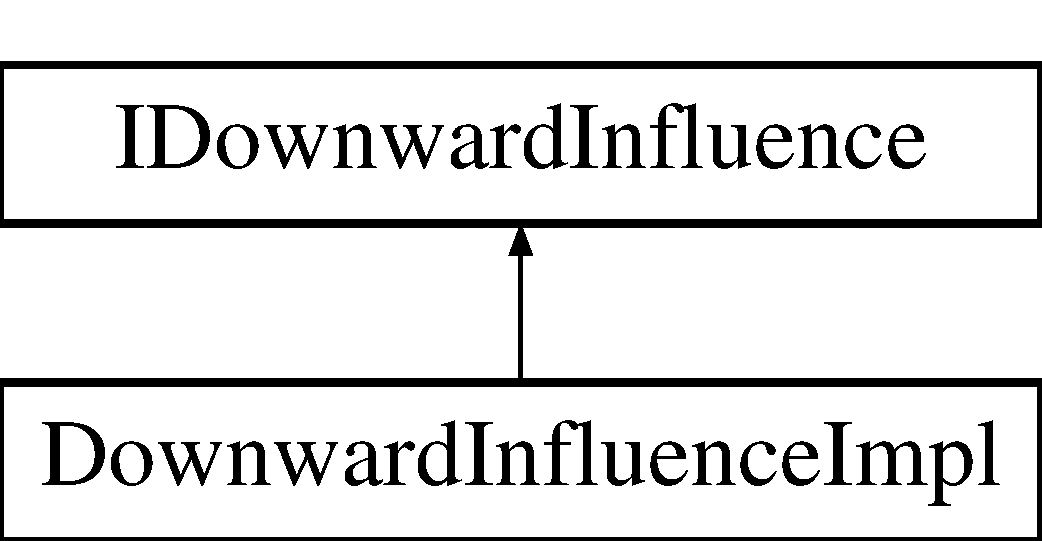
\includegraphics[height=2.000000cm]{classIDownwardInfluence}
\end{center}
\end{figure}
\subsection*{Public Member Functions}
\begin{DoxyCompactItemize}
\item 
{\bfseries I\+Downward\+Influence} (\hyperlink{classNode}{Node} $\ast$node)\hypertarget{classIDownwardInfluence_a7d5d6eb85ad3628703de8792dcebb9b5}{}\label{classIDownwardInfluence_a7d5d6eb85ad3628703de8792dcebb9b5}

\item 
virtual void {\bfseries calculate\+Downward\+Influence} ()=0\hypertarget{classIDownwardInfluence_ae6810945efb7ceb9b6e351c62bacd453}{}\label{classIDownwardInfluence_ae6810945efb7ceb9b6e351c62bacd453}

\end{DoxyCompactItemize}
\subsection*{Protected Attributes}
\begin{DoxyCompactItemize}
\item 
\hyperlink{classNode}{Node} $\ast$ {\bfseries m\+Node}\hypertarget{classIDownwardInfluence_aad871e67e020cdc589deb3739f8548a0}{}\label{classIDownwardInfluence_aad871e67e020cdc589deb3739f8548a0}

\end{DoxyCompactItemize}


The documentation for this class was generated from the following file\+:\begin{DoxyCompactItemize}
\item 
/home/mate/\+Documents/\+Programming/\+Research/\+Multilayer\+Network\+Model/\+Multilayer\+Network\+Model/src/core/include/I\+Downward\+Influence.\+hh\end{DoxyCompactItemize}

\hypertarget{classIDynamicalEquationGenerator}{}\section{I\+Dynamical\+Equation\+Generator Class Reference}
\label{classIDynamicalEquationGenerator}\index{I\+Dynamical\+Equation\+Generator@{I\+Dynamical\+Equation\+Generator}}
Inheritance diagram for I\+Dynamical\+Equation\+Generator\+:\begin{figure}[H]
\begin{center}
\leavevmode
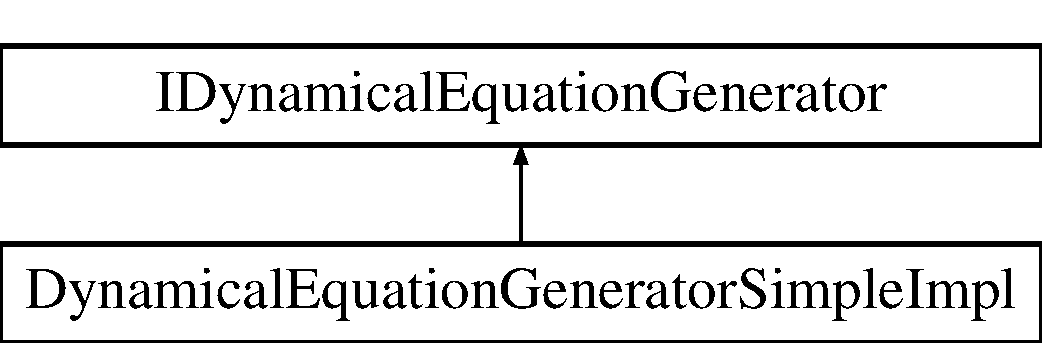
\includegraphics[height=2.000000cm]{classIDynamicalEquationGenerator}
\end{center}
\end{figure}
\subsection*{Public Member Functions}
\begin{DoxyCompactItemize}
\item 
{\bfseries I\+Dynamical\+Equation\+Generator} (\hyperlink{classMultilayerNetwork}{Multilayer\+Network} $\ast$multilayer\+Network)\hypertarget{classIDynamicalEquationGenerator_a7c4ee27a9153c6c71c56363509e9db50}{}\label{classIDynamicalEquationGenerator_a7c4ee27a9153c6c71c56363509e9db50}

\item 
virtual void {\bfseries generate\+Dynamical\+Equations} ()=0\hypertarget{classIDynamicalEquationGenerator_a23867fb164b2e17a98f2acde2f6d658e}{}\label{classIDynamicalEquationGenerator_a23867fb164b2e17a98f2acde2f6d658e}

\end{DoxyCompactItemize}
\subsection*{Protected Attributes}
\begin{DoxyCompactItemize}
\item 
\hyperlink{classMultilayerNetwork}{Multilayer\+Network} $\ast$ {\bfseries m\+Multilayer\+Network}\hypertarget{classIDynamicalEquationGenerator_aa20ebd4982dc045c28dba4e0fb63c585}{}\label{classIDynamicalEquationGenerator_aa20ebd4982dc045c28dba4e0fb63c585}

\end{DoxyCompactItemize}


The documentation for this class was generated from the following file\+:\begin{DoxyCompactItemize}
\item 
/home/mate/\+Documents/\+Programming/\+Research/\+Multilayer\+Network\+Model/\+Multilayer\+Network\+Model/sources/generators/include/I\+Dynamical\+Equation\+Generator.\+hh\end{DoxyCompactItemize}

\hypertarget{classIInitialConditionGenerator}{}\section{I\+Initial\+Condition\+Generator Class Reference}
\label{classIInitialConditionGenerator}\index{I\+Initial\+Condition\+Generator@{I\+Initial\+Condition\+Generator}}
Inheritance diagram for I\+Initial\+Condition\+Generator\+:\begin{figure}[H]
\begin{center}
\leavevmode
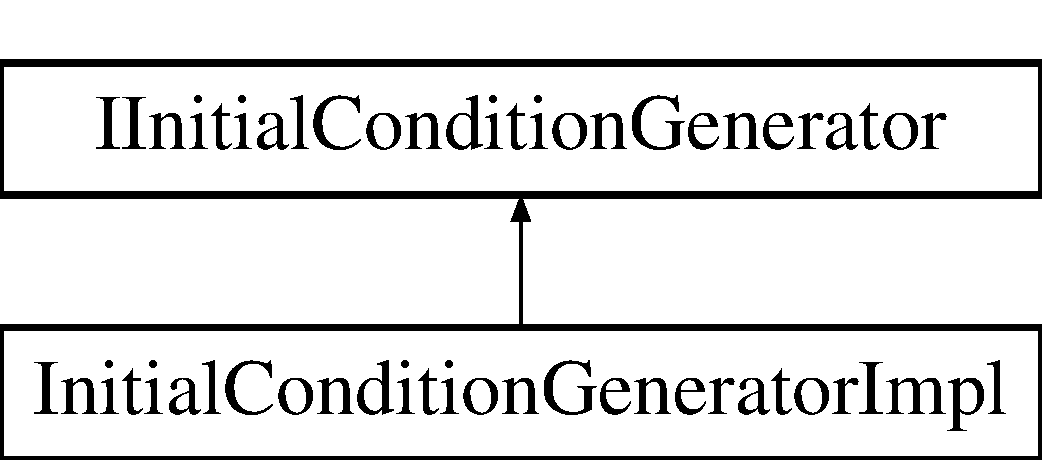
\includegraphics[height=2.000000cm]{classIInitialConditionGenerator}
\end{center}
\end{figure}
\subsection*{Public Member Functions}
\begin{DoxyCompactItemize}
\item 
{\bfseries I\+Initial\+Condition\+Generator} (\hyperlink{classMultilayerNetwork}{Multilayer\+Network} $\ast$multilayer\+Network)\hypertarget{classIInitialConditionGenerator_a23bef59a851914a65f67c2bd7736ad37}{}\label{classIInitialConditionGenerator_a23bef59a851914a65f67c2bd7736ad37}

\item 
virtual void {\bfseries generate\+Initial\+Condition} ()=0\hypertarget{classIInitialConditionGenerator_aaee78296548634e00150023baa051e52}{}\label{classIInitialConditionGenerator_aaee78296548634e00150023baa051e52}

\end{DoxyCompactItemize}
\subsection*{Protected Attributes}
\begin{DoxyCompactItemize}
\item 
\hyperlink{classMultilayerNetwork}{Multilayer\+Network} $\ast$ {\bfseries m\+Multilayer\+Network}\hypertarget{classIInitialConditionGenerator_a7144fdc9973103d6b377958868b4b387}{}\label{classIInitialConditionGenerator_a7144fdc9973103d6b377958868b4b387}

\end{DoxyCompactItemize}


The documentation for this class was generated from the following file\+:\begin{DoxyCompactItemize}
\item 
/home/mate/\+Documents/\+Programming/\+Research/\+Multilayer\+Network\+Model/\+Multilayer\+Network\+Model/src/generators/include/I\+Initial\+Condition\+Generator.\+hh\end{DoxyCompactItemize}

\hypertarget{classInitialConditionGeneratorImpl}{}\section{Initial\+Condition\+Generator\+Impl Class Reference}
\label{classInitialConditionGeneratorImpl}\index{Initial\+Condition\+Generator\+Impl@{Initial\+Condition\+Generator\+Impl}}
Inheritance diagram for Initial\+Condition\+Generator\+Impl\+:\begin{figure}[H]
\begin{center}
\leavevmode
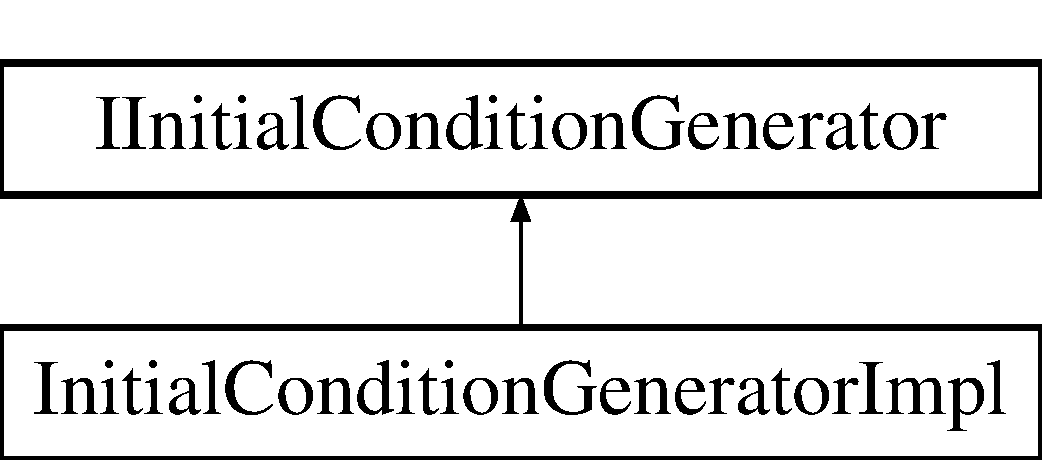
\includegraphics[height=2.000000cm]{classInitialConditionGeneratorImpl}
\end{center}
\end{figure}
\subsection*{Public Member Functions}
\begin{DoxyCompactItemize}
\item 
{\bfseries Initial\+Condition\+Generator\+Impl} (\hyperlink{classMultilayerNetwork}{Multilayer\+Network} $\ast$multilayer\+Network)\hypertarget{classInitialConditionGeneratorImpl_a07647da5a3eece4804a53135bb54c738}{}\label{classInitialConditionGeneratorImpl_a07647da5a3eece4804a53135bb54c738}

\item 
void {\bfseries generate\+Initial\+Condition} ()\hypertarget{classInitialConditionGeneratorImpl_ab296cde00693ad9b2b0199c69a3c3326}{}\label{classInitialConditionGeneratorImpl_ab296cde00693ad9b2b0199c69a3c3326}

\end{DoxyCompactItemize}
\subsection*{Additional Inherited Members}


The documentation for this class was generated from the following files\+:\begin{DoxyCompactItemize}
\item 
/home/mate/\+Documents/\+Programming/\+Research/\+Multilayer\+Network\+Model/\+Multilayer\+Network\+Model/sources/generators/include/Initial\+Condition\+Generator\+Impl.\+hh\item 
/home/mate/\+Documents/\+Programming/\+Research/\+Multilayer\+Network\+Model/\+Multilayer\+Network\+Model/sources/generators/src/Initial\+Condition\+Generator\+Impl.\+cc\end{DoxyCompactItemize}

\hypertarget{classEzAquarii_1_1Interpreter}{}\section{Ez\+Aquarii\+:\+:Interpreter Class Reference}
\label{classEzAquarii_1_1Interpreter}\index{Ez\+Aquarii\+::\+Interpreter@{Ez\+Aquarii\+::\+Interpreter}}
\subsection*{Public Member Functions}
\begin{DoxyCompactItemize}
\item 
int {\bfseries parse} ()\hypertarget{classEzAquarii_1_1Interpreter_aa88f207642eaa0a2d04cf5d050957c1a}{}\label{classEzAquarii_1_1Interpreter_aa88f207642eaa0a2d04cf5d050957c1a}

\item 
\hyperlink{classCalculationNode}{Calculation\+Node} $\ast$ {\bfseries get\+Base\+Calculation\+Node} ()\hypertarget{classEzAquarii_1_1Interpreter_ac861c17080e13412300574e96612d114}{}\label{classEzAquarii_1_1Interpreter_ac861c17080e13412300574e96612d114}

\item 
void {\bfseries switch\+Input\+Stream} (std\+::istringstream $\ast$is)\hypertarget{classEzAquarii_1_1Interpreter_a4dc3765926d0bf9d103859f713bd1e32}{}\label{classEzAquarii_1_1Interpreter_a4dc3765926d0bf9d103859f713bd1e32}

\item 
void {\bfseries print\+Calculation\+Nodes} ()\hypertarget{classEzAquarii_1_1Interpreter_ab67d30dbcf20022891d6cd58615db65c}{}\label{classEzAquarii_1_1Interpreter_ab67d30dbcf20022891d6cd58615db65c}

\end{DoxyCompactItemize}
\subsection*{Friends}
\begin{DoxyCompactItemize}
\item 
class {\bfseries Parser}\hypertarget{classEzAquarii_1_1Interpreter_ab80291af9c262f63b83fa9c16f12014d}{}\label{classEzAquarii_1_1Interpreter_ab80291af9c262f63b83fa9c16f12014d}

\item 
class {\bfseries Scanner}\hypertarget{classEzAquarii_1_1Interpreter_af4a8f36320cb35fb6b88d6b9a33cb524}{}\label{classEzAquarii_1_1Interpreter_af4a8f36320cb35fb6b88d6b9a33cb524}

\end{DoxyCompactItemize}


The documentation for this class was generated from the following files\+:\begin{DoxyCompactItemize}
\item 
/home/mate/\+Documents/\+Programming/\+Research/\+Multilayer\+Network\+Model/\+Multilayer\+Network\+Model/src/parser/include/interpreter.\+h\item 
/home/mate/\+Documents/\+Programming/\+Research/\+Multilayer\+Network\+Model/\+Multilayer\+Network\+Model/src/parser/src/interpreter.\+cpp\end{DoxyCompactItemize}

\hypertarget{classIStructureGenerator}{}\section{I\+Structure\+Generator Class Reference}
\label{classIStructureGenerator}\index{I\+Structure\+Generator@{I\+Structure\+Generator}}
Inheritance diagram for I\+Structure\+Generator\+:\begin{figure}[H]
\begin{center}
\leavevmode
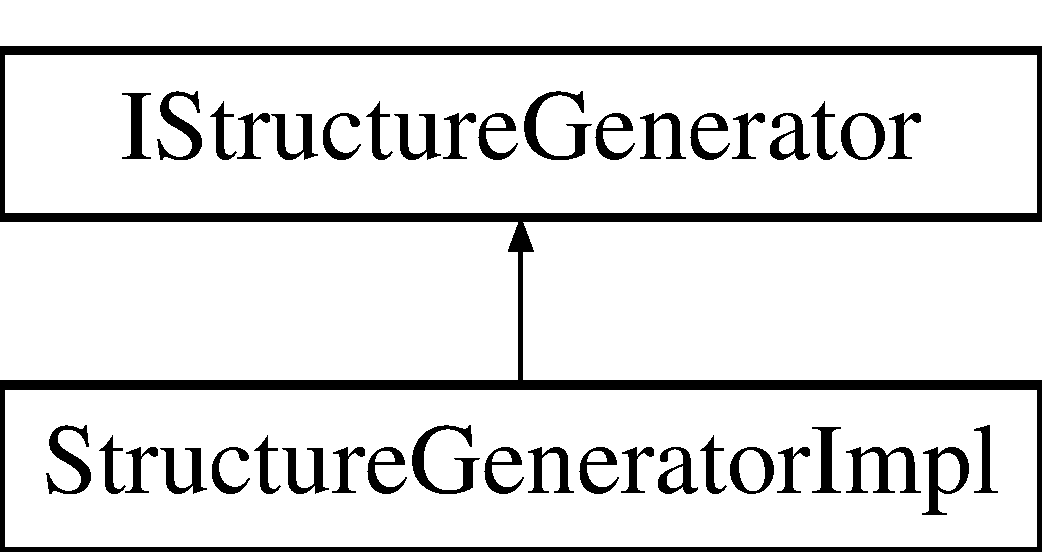
\includegraphics[height=2.000000cm]{classIStructureGenerator}
\end{center}
\end{figure}
\subsection*{Public Member Functions}
\begin{DoxyCompactItemize}
\item 
{\bfseries I\+Structure\+Generator} (\hyperlink{classMultilayerNetwork}{Multilayer\+Network} $\ast$multilayer\+Network)\hypertarget{classIStructureGenerator_af1536f217b3898a794a23417b3a0a2ed}{}\label{classIStructureGenerator_af1536f217b3898a794a23417b3a0a2ed}

\item 
virtual void {\bfseries generate\+Structure} ()=0\hypertarget{classIStructureGenerator_a6fd7b5ad3b544e5069e83a5fc62e249c}{}\label{classIStructureGenerator_a6fd7b5ad3b544e5069e83a5fc62e249c}

\end{DoxyCompactItemize}
\subsection*{Protected Attributes}
\begin{DoxyCompactItemize}
\item 
\hyperlink{classMultilayerNetwork}{Multilayer\+Network} $\ast$ {\bfseries m\+Multilayer\+Network}\hypertarget{classIStructureGenerator_af3bd39449b5256b4e4505005c34f33c4}{}\label{classIStructureGenerator_af3bd39449b5256b4e4505005c34f33c4}

\end{DoxyCompactItemize}


The documentation for this class was generated from the following file\+:\begin{DoxyCompactItemize}
\item 
/home/mate/\+Documents/\+Programming/\+Research/\+Multilayer\+Network\+Model/\+Multilayer\+Network\+Model/sources/generators/include/I\+Structure\+Generator.\+hh\end{DoxyCompactItemize}

\hypertarget{classIUpwardInfluence}{}\section{I\+Upward\+Influence Class Reference}
\label{classIUpwardInfluence}\index{I\+Upward\+Influence@{I\+Upward\+Influence}}
Inheritance diagram for I\+Upward\+Influence\+:\begin{figure}[H]
\begin{center}
\leavevmode
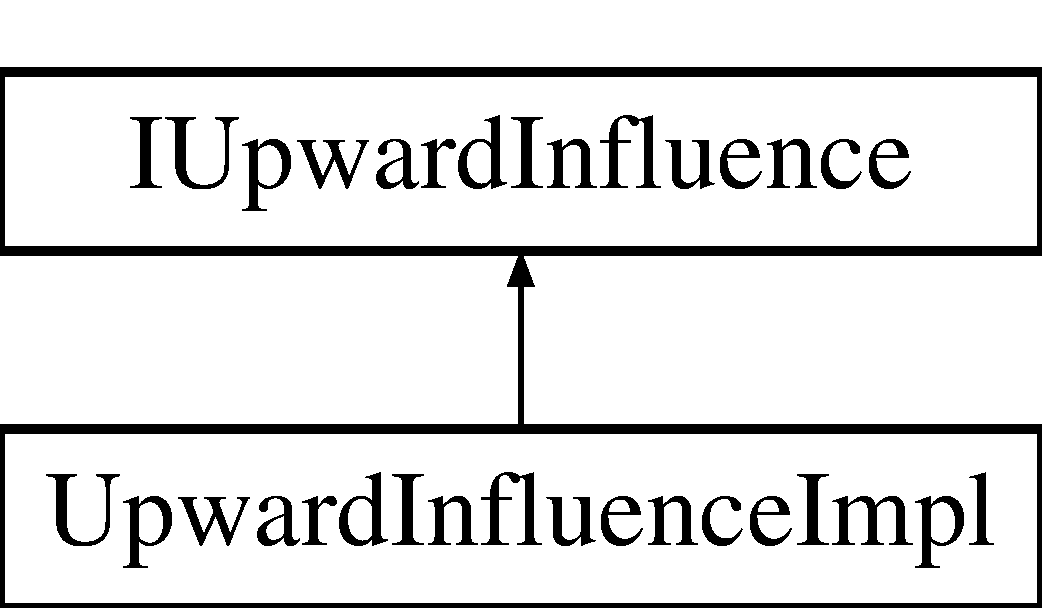
\includegraphics[height=2.000000cm]{classIUpwardInfluence}
\end{center}
\end{figure}
\subsection*{Public Member Functions}
\begin{DoxyCompactItemize}
\item 
{\bfseries I\+Upward\+Influence} (\hyperlink{classNode}{Node} $\ast$node)\hypertarget{classIUpwardInfluence_adc85bc94bdd2b99e474db59901e1cc7b}{}\label{classIUpwardInfluence_adc85bc94bdd2b99e474db59901e1cc7b}

\item 
virtual void {\bfseries calculate\+Upward\+Influence} ()=0\hypertarget{classIUpwardInfluence_adcb9517abfc35398e212fd47af22fdb0}{}\label{classIUpwardInfluence_adcb9517abfc35398e212fd47af22fdb0}

\end{DoxyCompactItemize}
\subsection*{Protected Attributes}
\begin{DoxyCompactItemize}
\item 
\hyperlink{classNode}{Node} $\ast$ {\bfseries m\+Node}\hypertarget{classIUpwardInfluence_aba560a3989e018d2526b14ad91d52ea4}{}\label{classIUpwardInfluence_aba560a3989e018d2526b14ad91d52ea4}

\end{DoxyCompactItemize}


The documentation for this class was generated from the following file\+:\begin{DoxyCompactItemize}
\item 
/home/mate/\+Documents/\+Programming/\+Research/\+Multilayer\+Network\+Model/\+Multilayer\+Network\+Model/src/core/include/I\+Upward\+Influence.\+hh\end{DoxyCompactItemize}

\hypertarget{classIVectorFieldReconfiguration}{}\section{I\+Vector\+Field\+Reconfiguration Class Reference}
\label{classIVectorFieldReconfiguration}\index{I\+Vector\+Field\+Reconfiguration@{I\+Vector\+Field\+Reconfiguration}}
Inheritance diagram for I\+Vector\+Field\+Reconfiguration\+:\begin{figure}[H]
\begin{center}
\leavevmode
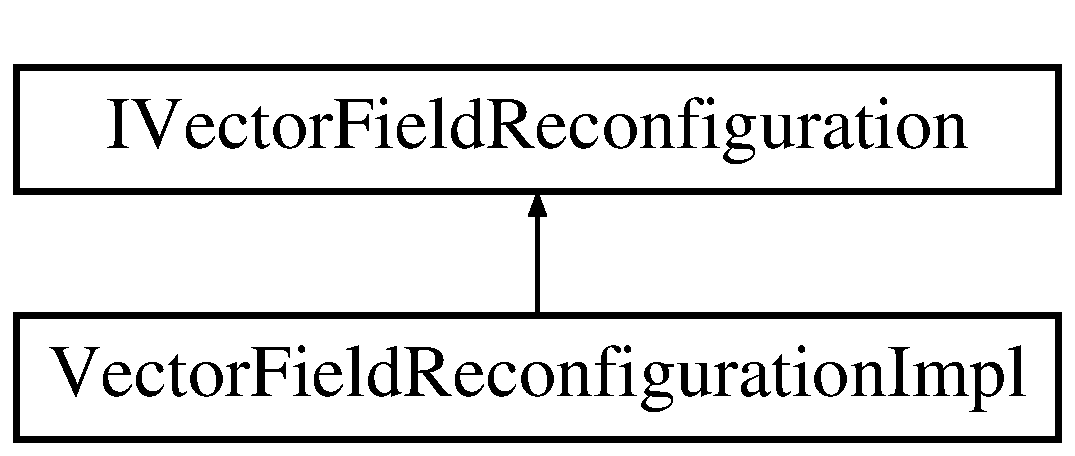
\includegraphics[height=2.000000cm]{classIVectorFieldReconfiguration}
\end{center}
\end{figure}
\subsection*{Public Member Functions}
\begin{DoxyCompactItemize}
\item 
{\bfseries I\+Vector\+Field\+Reconfiguration} (\hyperlink{classNode}{Node} $\ast$node)\hypertarget{classIVectorFieldReconfiguration_a6b663421658c873129a81c3597e0a4c1}{}\label{classIVectorFieldReconfiguration_a6b663421658c873129a81c3597e0a4c1}

\item 
virtual void {\bfseries calculate\+Vector\+Field\+Reconfiguration} ()=0\hypertarget{classIVectorFieldReconfiguration_a3d4ae2c51645c6e6e1955d7ea152ec04}{}\label{classIVectorFieldReconfiguration_a3d4ae2c51645c6e6e1955d7ea152ec04}

\end{DoxyCompactItemize}
\subsection*{Protected Attributes}
\begin{DoxyCompactItemize}
\item 
\hyperlink{classNode}{Node} $\ast$ {\bfseries m\+Node}\hypertarget{classIVectorFieldReconfiguration_a3a8452d0f63f8c9e05e1ad6faab26325}{}\label{classIVectorFieldReconfiguration_a3a8452d0f63f8c9e05e1ad6faab26325}

\end{DoxyCompactItemize}


The documentation for this class was generated from the following file\+:\begin{DoxyCompactItemize}
\item 
/home/mate/\+Documents/\+Programming/\+Research/\+Multilayer\+Network\+Model/\+Multilayer\+Network\+Model/src/core/include/I\+Vector\+Field\+Reconfiguration.\+hh\end{DoxyCompactItemize}

\hypertarget{classLayer}{}\section{Layer Class Reference}
\label{classLayer}\index{Layer@{Layer}}
\subsection*{Public Member Functions}
\begin{DoxyCompactItemize}
\item 
{\bfseries Layer} (int)\hypertarget{classLayer_a3f0552558b7008ebe37b74d55181d2a8}{}\label{classLayer_a3f0552558b7008ebe37b74d55181d2a8}

\item 
void {\bfseries add\+Network} (int network\+Id)\hypertarget{classLayer_ae76589e097e0fc8d3fc0d16c83670a5c}{}\label{classLayer_ae76589e097e0fc8d3fc0d16c83670a5c}

\item 
std\+::vector$<$ \hyperlink{classNetwork}{Network} $\ast$ $>$ {\bfseries get\+Networks} (void) const \hypertarget{classLayer_a7c8fe4f0a91522c0ffbb4b6ed3d507f1}{}\label{classLayer_a7c8fe4f0a91522c0ffbb4b6ed3d507f1}

\item 
int {\bfseries get\+Id} (void) const \hypertarget{classLayer_a00123131915f8bef4bf58bda3229e80c}{}\label{classLayer_a00123131915f8bef4bf58bda3229e80c}

\end{DoxyCompactItemize}
\subsection*{Friends}
\begin{DoxyCompactItemize}
\item 
bool {\bfseries operator==} (const \hyperlink{classLayer}{Layer} \&layer1, const \hyperlink{classLayer}{Layer} \&layer2)\hypertarget{classLayer_aca6ebc1f2e29896977fd9434db21761b}{}\label{classLayer_aca6ebc1f2e29896977fd9434db21761b}

\end{DoxyCompactItemize}


The documentation for this class was generated from the following files\+:\begin{DoxyCompactItemize}
\item 
/home/mate/\+Documents/\+Programming/\+Research/\+Multilayer\+Network\+Model/\+Multilayer\+Network\+Model/src/core/include/Layer.\+hh\item 
/home/mate/\+Documents/\+Programming/\+Research/\+Multilayer\+Network\+Model/\+Multilayer\+Network\+Model/src/core/src/Layer.\+cc\end{DoxyCompactItemize}

\hypertarget{classEzAquarii_1_1location}{}\section{Ez\+Aquarii\+:\+:location Class Reference}
\label{classEzAquarii_1_1location}\index{Ez\+Aquarii\+::location@{Ez\+Aquarii\+::location}}


Abstract a location.  




{\ttfamily \#include $<$location.\+hh$>$}

\subsection*{Public Member Functions}
\begin{DoxyCompactItemize}
\item 
\hyperlink{classEzAquarii_1_1location_ad1317d935037a54e328f1b540d296e76}{location} (const \hyperlink{classEzAquarii_1_1position}{position} \&b, const \hyperlink{classEzAquarii_1_1position}{position} \&e)\hypertarget{classEzAquarii_1_1location_ad1317d935037a54e328f1b540d296e76}{}\label{classEzAquarii_1_1location_ad1317d935037a54e328f1b540d296e76}

\begin{DoxyCompactList}\small\item\em Construct a location from {\itshape b} to {\itshape e}. \end{DoxyCompactList}\item 
\hyperlink{classEzAquarii_1_1location_a53601244b738c831abb3a4fa6b6879a9}{location} (const \hyperlink{classEzAquarii_1_1position}{position} \&p=\hyperlink{classEzAquarii_1_1position}{position}())\hypertarget{classEzAquarii_1_1location_a53601244b738c831abb3a4fa6b6879a9}{}\label{classEzAquarii_1_1location_a53601244b738c831abb3a4fa6b6879a9}

\begin{DoxyCompactList}\small\item\em Construct a 0-\/width location in {\itshape p}. \end{DoxyCompactList}\item 
\hyperlink{classEzAquarii_1_1location_a0c8659136500d18d4b2bca8077074c5b}{location} (std\+::string $\ast$f, unsigned int l=1u, unsigned int c=1u)\hypertarget{classEzAquarii_1_1location_a0c8659136500d18d4b2bca8077074c5b}{}\label{classEzAquarii_1_1location_a0c8659136500d18d4b2bca8077074c5b}

\begin{DoxyCompactList}\small\item\em Construct a 0-\/width location in {\itshape f}, {\itshape l}, {\itshape c}. \end{DoxyCompactList}\item 
void \hyperlink{classEzAquarii_1_1location_ab7e7119497ff53c35cf63c5589c598e6}{initialize} (std\+::string $\ast$f=Y\+Y\+\_\+\+N\+U\+L\+L\+P\+TR, unsigned int l=1u, unsigned int c=1u)\hypertarget{classEzAquarii_1_1location_ab7e7119497ff53c35cf63c5589c598e6}{}\label{classEzAquarii_1_1location_ab7e7119497ff53c35cf63c5589c598e6}

\begin{DoxyCompactList}\small\item\em Initialization. \end{DoxyCompactList}\end{DoxyCompactItemize}
\begin{Indent}{\bf Line and Column related manipulators}\par
\begin{DoxyCompactItemize}
\item 
void \hyperlink{classEzAquarii_1_1location_acf36facf71d7a487c5f0b6d842cc131e}{step} ()\hypertarget{classEzAquarii_1_1location_acf36facf71d7a487c5f0b6d842cc131e}{}\label{classEzAquarii_1_1location_acf36facf71d7a487c5f0b6d842cc131e}

\begin{DoxyCompactList}\small\item\em Reset initial location to final location. \end{DoxyCompactList}\item 
void \hyperlink{classEzAquarii_1_1location_aa28f227132ae57c28625c819ce4f0cd0}{columns} (int count=1)\hypertarget{classEzAquarii_1_1location_aa28f227132ae57c28625c819ce4f0cd0}{}\label{classEzAquarii_1_1location_aa28f227132ae57c28625c819ce4f0cd0}

\begin{DoxyCompactList}\small\item\em Extend the current location to the C\+O\+U\+NT next columns. \end{DoxyCompactList}\item 
void \hyperlink{classEzAquarii_1_1location_ad63e80d670f482a693e727c9a0f4e7a0}{lines} (int count=1)\hypertarget{classEzAquarii_1_1location_ad63e80d670f482a693e727c9a0f4e7a0}{}\label{classEzAquarii_1_1location_ad63e80d670f482a693e727c9a0f4e7a0}

\begin{DoxyCompactList}\small\item\em Extend the current location to the C\+O\+U\+NT next lines. \end{DoxyCompactList}\end{DoxyCompactItemize}
\end{Indent}
\subsection*{Public Attributes}
\begin{DoxyCompactItemize}
\item 
\hyperlink{classEzAquarii_1_1position}{position} \hyperlink{classEzAquarii_1_1location_a44a3986e4a47d2e1a42b6d4ef4d325a7}{begin}\hypertarget{classEzAquarii_1_1location_a44a3986e4a47d2e1a42b6d4ef4d325a7}{}\label{classEzAquarii_1_1location_a44a3986e4a47d2e1a42b6d4ef4d325a7}

\begin{DoxyCompactList}\small\item\em Beginning of the located region. \end{DoxyCompactList}\item 
\hyperlink{classEzAquarii_1_1position}{position} \hyperlink{classEzAquarii_1_1location_acc6895050d9a3a5de820d0b482d9baf0}{end}\hypertarget{classEzAquarii_1_1location_acc6895050d9a3a5de820d0b482d9baf0}{}\label{classEzAquarii_1_1location_acc6895050d9a3a5de820d0b482d9baf0}

\begin{DoxyCompactList}\small\item\em End of the located region. \end{DoxyCompactList}\end{DoxyCompactItemize}


\subsection{Detailed Description}
Abstract a location. 

The documentation for this class was generated from the following file\+:\begin{DoxyCompactItemize}
\item 
/home/mate/\+Documents/\+Programming/\+Research/\+Multilayer\+Network\+Model/\+Multilayer\+Network\+Model/src/parser/include/\hyperlink{location_8hh}{location.\+hh}\end{DoxyCompactItemize}

\hypertarget{classMultilayerNetwork}{}\section{Multilayer\+Network Class Reference}
\label{classMultilayerNetwork}\index{Multilayer\+Network@{Multilayer\+Network}}
\subsection*{Public Member Functions}
\begin{DoxyCompactItemize}
\item 
void \hyperlink{classMultilayerNetwork_a229198446718a0bf87d872ea04f5308a}{add\+Layer} (int layer\+Id)
\item 
std\+::vector$<$ \hyperlink{classLayer}{Layer} $\ast$ $>$ {\bfseries get\+Layers} (void) const \hypertarget{classMultilayerNetwork_ad4ec3500f8c0b436ba738dcd5b533ba6}{}\label{classMultilayerNetwork_ad4ec3500f8c0b436ba738dcd5b533ba6}

\item 
void \hyperlink{classMultilayerNetwork_a8b52de3dbb17a23b7c86708ad53ba161}{step} (void)
\item 
void {\bfseries save} (const char $\ast$filename)\hypertarget{classMultilayerNetwork_ad5e402faebd6fb5b44616f549286757b}{}\label{classMultilayerNetwork_ad5e402faebd6fb5b44616f549286757b}

\item 
void {\bfseries load} (const char $\ast$filename)\hypertarget{classMultilayerNetwork_a6649a568665867114ddebe7b4b0726f7}{}\label{classMultilayerNetwork_a6649a568665867114ddebe7b4b0726f7}

\item 
void {\bfseries save\+State} (std\+::string filename=\char`\"{}\char`\"{})\hypertarget{classMultilayerNetwork_a4723e9478fe2a78bcf35a540869d66a4}{}\label{classMultilayerNetwork_a4723e9478fe2a78bcf35a540869d66a4}

\item 
void {\bfseries load\+State} (const char $\ast$filename)\hypertarget{classMultilayerNetwork_a2536024138714e0ddc51bb4b1ae79395}{}\label{classMultilayerNetwork_a2536024138714e0ddc51bb4b1ae79395}

\item 
void \hyperlink{classMultilayerNetwork_ab21e50242eea4221aab415e5b2a5a326}{load\+Nodes\+To\+All\+Equations} (void)
\item 
void \hyperlink{classMultilayerNetwork_a1d00f683f9d07fc715b8c2e4786884c8}{shift\+Buffers} (void)
\item 
void {\bfseries collect\+Nodes} (std\+::map$<$ int, \hyperlink{classNode}{Node} $\ast$ $>$ \&nodes\+Map, std\+::vector$<$ int $>$ \&node\+Ids) const \hypertarget{classMultilayerNetwork_a336346cc9479828006fed64ce4f204e8}{}\label{classMultilayerNetwork_a336346cc9479828006fed64ce4f204e8}

\item 
void {\bfseries collect\+Networks} (std\+::map$<$ int, \hyperlink{classNetwork}{Network} $\ast$ $>$ \&networks\+Map, std\+::vector$<$ int $>$ \&network\+Ids) const \hypertarget{classMultilayerNetwork_a9e846141725eb38c565af6db4040cf34}{}\label{classMultilayerNetwork_a9e846141725eb38c565af6db4040cf34}

\end{DoxyCompactItemize}
\subsection*{Friends}
\begin{DoxyCompactItemize}
\item 
bool {\bfseries initial\+Conditions\+Equal} (const \hyperlink{classMultilayerNetwork}{Multilayer\+Network} \&multilayer\+Network1, const \hyperlink{classMultilayerNetwork}{Multilayer\+Network} \&multilayer\+Network2)\hypertarget{classMultilayerNetwork_a64691b2acaece23358b93a9e66625219}{}\label{classMultilayerNetwork_a64691b2acaece23358b93a9e66625219}

\item 
bool {\bfseries dynamical\+Equations\+Equal} (const \hyperlink{classMultilayerNetwork}{Multilayer\+Network} \&multilayer\+Network1, const \hyperlink{classMultilayerNetwork}{Multilayer\+Network} \&multilayer\+Network2)\hypertarget{classMultilayerNetwork_ab9211d4a43da6142bc9acaa862a27bc0}{}\label{classMultilayerNetwork_ab9211d4a43da6142bc9acaa862a27bc0}

\item 
std\+::ostream \& {\bfseries operator$<$$<$} (std\+::ostream \&os, const \hyperlink{classMultilayerNetwork}{Multilayer\+Network} \&multilayer\+Network)\hypertarget{classMultilayerNetwork_a42b39b2faefcb63564d2e4ba5cfeac26}{}\label{classMultilayerNetwork_a42b39b2faefcb63564d2e4ba5cfeac26}

\item 
bool {\bfseries operator==} (const \hyperlink{classMultilayerNetwork}{Multilayer\+Network} \&multilayer\+Network1, const \hyperlink{classMultilayerNetwork}{Multilayer\+Network} \&multilayer\+Network2)\hypertarget{classMultilayerNetwork_a63e44ec945c844ee62bb16debee88369}{}\label{classMultilayerNetwork_a63e44ec945c844ee62bb16debee88369}

\end{DoxyCompactItemize}


\subsection{Member Function Documentation}
\index{Multilayer\+Network@{Multilayer\+Network}!add\+Layer@{add\+Layer}}
\index{add\+Layer@{add\+Layer}!Multilayer\+Network@{Multilayer\+Network}}
\subsubsection[{\texorpdfstring{add\+Layer(int layer\+Id)}{addLayer(int layerId)}}]{\setlength{\rightskip}{0pt plus 5cm}void Multilayer\+Network\+::add\+Layer (
\begin{DoxyParamCaption}
\item[{int}]{layer\+Id}
\end{DoxyParamCaption}
)}\hypertarget{classMultilayerNetwork_a229198446718a0bf87d872ea04f5308a}{}\label{classMultilayerNetwork_a229198446718a0bf87d872ea04f5308a}
Adds a layer to the multilayer network. 
\begin{DoxyParams}{Parameters}
{\em layer\+Id} & the ID of the newly added layer \\
\hline
\end{DoxyParams}
\index{Multilayer\+Network@{Multilayer\+Network}!load\+Nodes\+To\+All\+Equations@{load\+Nodes\+To\+All\+Equations}}
\index{load\+Nodes\+To\+All\+Equations@{load\+Nodes\+To\+All\+Equations}!Multilayer\+Network@{Multilayer\+Network}}
\subsubsection[{\texorpdfstring{load\+Nodes\+To\+All\+Equations(void)}{loadNodesToAllEquations(void)}}]{\setlength{\rightskip}{0pt plus 5cm}void Multilayer\+Network\+::load\+Nodes\+To\+All\+Equations (
\begin{DoxyParamCaption}
\item[{void}]{}
\end{DoxyParamCaption}
)}\hypertarget{classMultilayerNetwork_ab21e50242eea4221aab415e5b2a5a326}{}\label{classMultilayerNetwork_ab21e50242eea4221aab415e5b2a5a326}
Calculation\+Nodes with type ID need to contain the pointer to the \hyperlink{classNode}{Node} they represent. This function loads all \hyperlink{classNode}{Node} objects to their representing Calculation\+Nodes. \index{Multilayer\+Network@{Multilayer\+Network}!shift\+Buffers@{shift\+Buffers}}
\index{shift\+Buffers@{shift\+Buffers}!Multilayer\+Network@{Multilayer\+Network}}
\subsubsection[{\texorpdfstring{shift\+Buffers(void)}{shiftBuffers(void)}}]{\setlength{\rightskip}{0pt plus 5cm}void Multilayer\+Network\+::shift\+Buffers (
\begin{DoxyParamCaption}
\item[{void}]{}
\end{DoxyParamCaption}
)}\hypertarget{classMultilayerNetwork_a1d00f683f9d07fc715b8c2e4786884c8}{}\label{classMultilayerNetwork_a1d00f683f9d07fc715b8c2e4786884c8}
When the end of buffers is reached i.\+e. they are filled with the previous values of the nodes, the contents of the current buffers is writen to a file, and the buffers are set back to all 0 elements, except for the first two values that contain the end values of the previous buffer. \index{Multilayer\+Network@{Multilayer\+Network}!step@{step}}
\index{step@{step}!Multilayer\+Network@{Multilayer\+Network}}
\subsubsection[{\texorpdfstring{step(void)}{step(void)}}]{\setlength{\rightskip}{0pt plus 5cm}void Multilayer\+Network\+::step (
\begin{DoxyParamCaption}
\item[{void}]{}
\end{DoxyParamCaption}
)}\hypertarget{classMultilayerNetwork_a8b52de3dbb17a23b7c86708ad53ba161}{}\label{classMultilayerNetwork_a8b52de3dbb17a23b7c86708ad53ba161}
Performs a single step on all of the nodes within the multilayer network. 

The documentation for this class was generated from the following files\+:\begin{DoxyCompactItemize}
\item 
/home/mate/\+Documents/\+Programming/\+Research/\+Multilayer\+Network\+Model/\+Multilayer\+Network\+Model/src/core/include/Multilayer\+Network.\+hh\item 
/home/mate/\+Documents/\+Programming/\+Research/\+Multilayer\+Network\+Model/\+Multilayer\+Network\+Model/src/core/src/Multilayer\+Network.\+cc\end{DoxyCompactItemize}

\hypertarget{classNetwork}{}\section{Network Class Reference}
\label{classNetwork}\index{Network@{Network}}
\subsection*{Public Member Functions}
\begin{DoxyCompactItemize}
\item 
{\bfseries Network} (int)\hypertarget{classNetwork_a30c34d28f6da478d4d7b597165dc95a9}{}\label{classNetwork_a30c34d28f6da478d4d7b597165dc95a9}

\item 
void {\bfseries add\+Node} (int node\+Id)\hypertarget{classNetwork_ae5cee65d8d673280142c6f1a9420b0e7}{}\label{classNetwork_ae5cee65d8d673280142c6f1a9420b0e7}

\item 
void {\bfseries add\+Edge} (int local\+Node\+Id1, int local\+Node\+Id2)\hypertarget{classNetwork_ae45cbbac2dd53ec1e1bb0c8074139d7d}{}\label{classNetwork_ae45cbbac2dd53ec1e1bb0c8074139d7d}

\item 
void {\bfseries remove\+Edge} (int local\+Node\+Id1, int local\+Node\+Id2)\hypertarget{classNetwork_a375aad913988baf7fefec77b7dd3a485}{}\label{classNetwork_a375aad913988baf7fefec77b7dd3a485}

\item 
void {\bfseries remove\+All\+Edges} ()\hypertarget{classNetwork_a900818896e85d83af131d590e68388f6}{}\label{classNetwork_a900818896e85d83af131d590e68388f6}

\item 
void {\bfseries assign\+To\+Node} (\hyperlink{classNode}{Node} $\ast$node)\hypertarget{classNetwork_a78e5489d4cf31b296366f5ccaede0fdf}{}\label{classNetwork_a78e5489d4cf31b296366f5ccaede0fdf}

\item 
void {\bfseries set\+Dynamical\+Equation} (int node\+Id, std\+::string str\+Equation)\hypertarget{classNetwork_a1e066354c2d7e40338ee2e5b3e974595}{}\label{classNetwork_a1e066354c2d7e40338ee2e5b3e974595}

\item 
void {\bfseries generate\+Connections} (void)\hypertarget{classNetwork_a2fcc69db1e696f07424a3fee766e125f}{}\label{classNetwork_a2fcc69db1e696f07424a3fee766e125f}

\item 
int {\bfseries get\+Id} (void) const \hypertarget{classNetwork_ae30196d51c9db40feaf93cde5508d106}{}\label{classNetwork_ae30196d51c9db40feaf93cde5508d106}

\item 
int {\bfseries get\+Local\+Id} (int id) const \hypertarget{classNetwork_a0b1b879abf7417e425325999a7919d15}{}\label{classNetwork_a0b1b879abf7417e425325999a7919d15}

\item 
\hyperlink{classNode}{Node} $\ast$ {\bfseries get\+Node\+Assigned} (void) const \hypertarget{classNetwork_a0c67b1e20e97cff7dedb84571936fd0b}{}\label{classNetwork_a0c67b1e20e97cff7dedb84571936fd0b}

\item 
std\+::vector$<$ \hyperlink{classNode}{Node} $\ast$ $>$ {\bfseries get\+Nodes} (void) const \hypertarget{classNetwork_afb787c0243504190c513013ca198e947}{}\label{classNetwork_afb787c0243504190c513013ca198e947}

\item 
std\+::vector$<$ \hyperlink{classNode}{Node} $\ast$ $>$ {\bfseries get\+Node\+Neighbors} (int node\+Id) const \hypertarget{classNetwork_afe7437019956a4677ef9d4df98c36730}{}\label{classNetwork_afe7437019956a4677ef9d4df98c36730}

\item 
\hyperlink{classDynamicalEquation}{Dynamical\+Equation} $\ast$ {\bfseries get\+Node\+Dynamical\+Equation} (int node\+Id) const \hypertarget{classNetwork_aecfd002e55cef6a23843d535e75f49e0}{}\label{classNetwork_aecfd002e55cef6a23843d535e75f49e0}

\item 
std\+::string {\bfseries get\+Node\+Dynamical\+Equation\+String} (int node\+Id) const \hypertarget{classNetwork_a69e8e7ddd08590f496eeb38d28e5f8dd}{}\label{classNetwork_a69e8e7ddd08590f496eeb38d28e5f8dd}

\item 
std\+::map$<$ int, double $>$ {\bfseries get\+Current\+State} (void) const \hypertarget{classNetwork_aa5727c4eb316f69edae5efee422d5c6a}{}\label{classNetwork_aa5727c4eb316f69edae5efee422d5c6a}

\item 
std\+::map$<$ int, double $>$ {\bfseries get\+Direction\+At\+State} (std\+::map$<$ int, double $>$ base\+Point\+Coordinates) const \hypertarget{classNetwork_a140759419ddad1c7dea5537e90c52572}{}\label{classNetwork_a140759419ddad1c7dea5537e90c52572}

\item 
\hyperlink{classNode}{Node} $\ast$ {\bfseries get\+Node\+By\+Id} (int node\+Id)\hypertarget{classNetwork_a0b983325b6f616ab86591f1a5c6b0d69}{}\label{classNetwork_a0b983325b6f616ab86591f1a5c6b0d69}

\end{DoxyCompactItemize}
\subsection*{Friends}
\begin{DoxyCompactItemize}
\item 
bool {\bfseries operator==} (const \hyperlink{classNetwork}{Network} \&network1, const \hyperlink{classNetwork}{Network} \&network2)\hypertarget{classNetwork_a7a1b02eac9fc1db7f981fe618019d99a}{}\label{classNetwork_a7a1b02eac9fc1db7f981fe618019d99a}

\end{DoxyCompactItemize}


The documentation for this class was generated from the following files\+:\begin{DoxyCompactItemize}
\item 
/home/mate/\+Documents/\+Programming/\+Research/\+Multilayer\+Network\+Model/\+Multilayer\+Network\+Model/src/core/include/Network.\+hh\item 
/home/mate/\+Documents/\+Programming/\+Research/\+Multilayer\+Network\+Model/\+Multilayer\+Network\+Model/src/core/src/Network.\+cc\end{DoxyCompactItemize}

\hypertarget{classNetworkModifier}{}\section{Network\+Modifier Class Reference}
\label{classNetworkModifier}\index{Network\+Modifier@{Network\+Modifier}}
\subsection*{Public Member Functions}
\begin{DoxyCompactItemize}
\item 
void {\bfseries modify\+Network} (\hyperlink{classNetwork}{Network} $\ast$network)\hypertarget{classNetworkModifier_a7d5af0b6aaa1a8365ff03749a7eb0376}{}\label{classNetworkModifier_a7d5af0b6aaa1a8365ff03749a7eb0376}

\item 
void {\bfseries copy\+Network} (\hyperlink{classNetwork}{Network} $\ast$old\+Network, \hyperlink{classNetwork}{Network} $\ast$new\+Network)\hypertarget{classNetworkModifier_a2ab956789ff4a954e0e3dd027512012b}{}\label{classNetworkModifier_a2ab956789ff4a954e0e3dd027512012b}

\item 
\hyperlink{classNode}{Node} $\ast$ {\bfseries choose\+Node} (\hyperlink{classNetwork}{Network} $\ast$network)\hypertarget{classNetworkModifier_a236ee2c417412e6333d4ed855bd9f88f}{}\label{classNetworkModifier_a236ee2c417412e6333d4ed855bd9f88f}

\item 
Modification\+Type {\bfseries choose\+Type} ()\hypertarget{classNetworkModifier_a11a4d6c3bb19cda4e9714ad296d72db1}{}\label{classNetworkModifier_a11a4d6c3bb19cda4e9714ad296d72db1}

\item 
void {\bfseries add\+Edge} (\hyperlink{classNetwork}{Network} $\ast$network, \hyperlink{classNode}{Node} $\ast$node)\hypertarget{classNetworkModifier_a7486df4a68343d65eb5bfb766d6959dd}{}\label{classNetworkModifier_a7486df4a68343d65eb5bfb766d6959dd}

\item 
void {\bfseries remove\+Edge} (\hyperlink{classNetwork}{Network} $\ast$network, \hyperlink{classNode}{Node} $\ast$node)\hypertarget{classNetworkModifier_a98de1cc69f96a312d823a18fb4e32125}{}\label{classNetworkModifier_a98de1cc69f96a312d823a18fb4e32125}

\item 
void {\bfseries add\+To\+Outer\+Block} (\hyperlink{classNetwork}{Network} $\ast$network, \hyperlink{classNode}{Node} $\ast$node)\hypertarget{classNetworkModifier_aa3003a2ca2ba2a64e3dfa52372befafe}{}\label{classNetworkModifier_aa3003a2ca2ba2a64e3dfa52372befafe}

\item 
void {\bfseries remove\+From\+Outer\+Block} (\hyperlink{classNetwork}{Network} $\ast$network, \hyperlink{classNode}{Node} $\ast$node)\hypertarget{classNetworkModifier_aa61381ec53af37a67753b95e162e2ee6}{}\label{classNetworkModifier_aa61381ec53af37a67753b95e162e2ee6}

\item 
void {\bfseries change\+Constant} (\hyperlink{classNetwork}{Network} $\ast$network, \hyperlink{classNode}{Node} $\ast$node)\hypertarget{classNetworkModifier_a574c45de40cd717c66412a821dec7720}{}\label{classNetworkModifier_a574c45de40cd717c66412a821dec7720}

\item 
void {\bfseries change\+Plus\+To\+Multiply} (\hyperlink{classNetwork}{Network} $\ast$network, \hyperlink{classNode}{Node} $\ast$node)\hypertarget{classNetworkModifier_af847b438d989b02336200e47f2059be5}{}\label{classNetworkModifier_af847b438d989b02336200e47f2059be5}

\item 
void {\bfseries change\+Multiply\+To\+Plus} (\hyperlink{classNetwork}{Network} $\ast$network, \hyperlink{classNode}{Node} $\ast$node)\hypertarget{classNetworkModifier_a50d862b93e5f37acaa073e5edaad9a2c}{}\label{classNetworkModifier_a50d862b93e5f37acaa073e5edaad9a2c}

\item 
\hyperlink{classNode}{Node} $\ast$ {\bfseries get\+Node\+\_\+add\+Edge} (\hyperlink{classNetwork}{Network} $\ast$network, \hyperlink{classNode}{Node} $\ast$node)\hypertarget{classNetworkModifier_a3ca48b0cbcc665ffadd0cebcc3a3e45b}{}\label{classNetworkModifier_a3ca48b0cbcc665ffadd0cebcc3a3e45b}

\item 
\hyperlink{classNode}{Node} $\ast$ {\bfseries get\+Node\+\_\+remove\+Edge} (\hyperlink{classNetwork}{Network} $\ast$network, \hyperlink{classNode}{Node} $\ast$node)\hypertarget{classNetworkModifier_a1519488c4c8787563bd37b8591f741bf}{}\label{classNetworkModifier_a1519488c4c8787563bd37b8591f741bf}

\item 
void {\bfseries get\+Locations\+\_\+add\+Edge} (\hyperlink{classCalculationNode}{Calculation\+Node} $\ast$calc\+Node, std\+::vector$<$ \hyperlink{classCalculationNode}{Calculation\+Node} $\ast$ $>$ \&locations)\hypertarget{classNetworkModifier_ac2e65c2e6985a1b6b8d90e0d5eac7b36}{}\label{classNetworkModifier_ac2e65c2e6985a1b6b8d90e0d5eac7b36}

\item 
void {\bfseries get\+Locations\+\_\+add\+To\+Outer\+Block} (\hyperlink{classCalculationNode}{Calculation\+Node} $\ast$calc\+Node, std\+::vector$<$ \hyperlink{classCalculationNode}{Calculation\+Node} $\ast$ $>$ \&locations)\hypertarget{classNetworkModifier_ac082b11da7cb452b9047eea94b0f1e37}{}\label{classNetworkModifier_ac082b11da7cb452b9047eea94b0f1e37}

\item 
void {\bfseries get\+Locations\+\_\+remove\+From\+Outer\+Block} (\hyperlink{classCalculationNode}{Calculation\+Node} $\ast$base\+Calc\+Node, \hyperlink{classCalculationNode}{Calculation\+Node} $\ast$calc\+Node, std\+::vector$<$ \hyperlink{classCalculationNode}{Calculation\+Node} $\ast$ $>$ \&locations)\hypertarget{classNetworkModifier_afe88d2366b6e5464b3e29a19fa1eeb1e}{}\label{classNetworkModifier_afe88d2366b6e5464b3e29a19fa1eeb1e}

\item 
void {\bfseries get\+Locations\+\_\+change\+Constant} (\hyperlink{classCalculationNode}{Calculation\+Node} $\ast$calc\+Node, std\+::vector$<$ \hyperlink{classCalculationNode}{Calculation\+Node} $\ast$ $>$ \&locations)\hypertarget{classNetworkModifier_a92f84a858a92dcd68e4ea252ea65f5a0}{}\label{classNetworkModifier_a92f84a858a92dcd68e4ea252ea65f5a0}

\item 
void {\bfseries get\+Locations\+\_\+change\+Plus\+To\+Multiply} (\hyperlink{classCalculationNode}{Calculation\+Node} $\ast$calc\+Node, std\+::vector$<$ \hyperlink{classCalculationNode}{Calculation\+Node} $\ast$ $>$ \&locations)\hypertarget{classNetworkModifier_a610cc380e39e047cdd2f716c75a657df}{}\label{classNetworkModifier_a610cc380e39e047cdd2f716c75a657df}

\item 
void {\bfseries get\+Locations\+\_\+change\+Multiply\+To\+Plus} (\hyperlink{classCalculationNode}{Calculation\+Node} $\ast$calc\+Node, std\+::vector$<$ \hyperlink{classCalculationNode}{Calculation\+Node} $\ast$ $>$ \&locations)\hypertarget{classNetworkModifier_ac396b8a961cd134496feb28b04f4a2ff}{}\label{classNetworkModifier_ac396b8a961cd134496feb28b04f4a2ff}

\item 
\hyperlink{classCalculationNode}{Calculation\+Node} $\ast$ {\bfseries specific\+\_\+add\+Edge} (\hyperlink{classCalculationNode}{Calculation\+Node} $\ast$base\+Calc\+Node, \hyperlink{classCalculationNode}{Calculation\+Node} $\ast$changing\+Calc\+Node, \hyperlink{classNode}{Node} $\ast$new\+Neighbor)\hypertarget{classNetworkModifier_a3e37a7d3d65e0162f2713da90a4a816a}{}\label{classNetworkModifier_a3e37a7d3d65e0162f2713da90a4a816a}

\item 
\hyperlink{classCalculationNode}{Calculation\+Node} $\ast$ {\bfseries specific\+\_\+remove\+Edge} (\hyperlink{classCalculationNode}{Calculation\+Node} $\ast$base\+Calc\+Node, \hyperlink{classCalculationNode}{Calculation\+Node} $\ast$changing\+Calc\+Node)\hypertarget{classNetworkModifier_a6f72ac88702c225e881964f178d63bd7}{}\label{classNetworkModifier_a6f72ac88702c225e881964f178d63bd7}

\item 
void {\bfseries specific\+\_\+change\+Constant} (\hyperlink{classCalculationNode}{Calculation\+Node} $\ast$changing\+Calc\+Node)\hypertarget{classNetworkModifier_a826ad8a3e5fd313e1f263a8088da55fe}{}\label{classNetworkModifier_a826ad8a3e5fd313e1f263a8088da55fe}

\item 
\hyperlink{classCalculationNode}{Calculation\+Node} $\ast$ {\bfseries specific\+\_\+change\+Plus\+To\+Multiply} (\hyperlink{classCalculationNode}{Calculation\+Node} $\ast$base\+Calc\+Node, \hyperlink{classCalculationNode}{Calculation\+Node} $\ast$changing\+Calc\+Node)\hypertarget{classNetworkModifier_aec5fb3ec5702d8ec879135ed9fd3fd59}{}\label{classNetworkModifier_aec5fb3ec5702d8ec879135ed9fd3fd59}

\item 
\hyperlink{classCalculationNode}{Calculation\+Node} $\ast$ {\bfseries specific\+\_\+change\+Multiply\+To\+Plus} (\hyperlink{classCalculationNode}{Calculation\+Node} $\ast$base\+Calc\+Node, \hyperlink{classCalculationNode}{Calculation\+Node} $\ast$changing\+Calc\+Node)\hypertarget{classNetworkModifier_a26e6b75e86ad045f64368add386aa2f8}{}\label{classNetworkModifier_a26e6b75e86ad045f64368add386aa2f8}

\item 
int {\bfseries number\+Of\+Type} (\hyperlink{classCalculationNode}{Calculation\+Node} $\ast$calc\+Node, Calc\+Node\+Types type)\hypertarget{classNetworkModifier_afecca95dfe9c898fd0fe3959f6846144}{}\label{classNetworkModifier_afecca95dfe9c898fd0fe3959f6846144}

\item 
\hyperlink{classCalculationNode}{Calculation\+Node} $\ast$ {\bfseries get\+Parent} (\hyperlink{classCalculationNode}{Calculation\+Node} $\ast$calc\+Node, \hyperlink{classCalculationNode}{Calculation\+Node} $\ast$child\+Calc\+Node)\hypertarget{classNetworkModifier_a8a8b86c2086a5c9102f123be773fc6f0}{}\label{classNetworkModifier_a8a8b86c2086a5c9102f123be773fc6f0}

\item 
void {\bfseries get\+Node\+Occurrences} (\hyperlink{classCalculationNode}{Calculation\+Node} $\ast$calc\+Node, std\+::vector$<$ \hyperlink{classCalculationNode}{Calculation\+Node} $\ast$ $>$ \&locations, int node\+Id)\hypertarget{classNetworkModifier_a2a8e14daebb6761624331a6c645cbe41}{}\label{classNetworkModifier_a2a8e14daebb6761624331a6c645cbe41}

\end{DoxyCompactItemize}


The documentation for this class was generated from the following files\+:\begin{DoxyCompactItemize}
\item 
/home/mate/\+Documents/\+Programming/\+Research/\+Multilayer\+Network\+Model/\+Multilayer\+Network\+Model/sources/core/\+Vector\+Field\+Reconfiguration/include/Network\+Modifier.\+hh\item 
/home/mate/\+Documents/\+Programming/\+Research/\+Multilayer\+Network\+Model/\+Multilayer\+Network\+Model/sources/core/\+Vector\+Field\+Reconfiguration/src/Network\+Modifier.\+cc\end{DoxyCompactItemize}

\hypertarget{classNetworkPopulationElement}{}\section{Network\+Population\+Element Class Reference}
\label{classNetworkPopulationElement}\index{Network\+Population\+Element@{Network\+Population\+Element}}
\subsection*{Public Member Functions}
\begin{DoxyCompactItemize}
\item 
{\bfseries Network\+Population\+Element} (\hyperlink{classNetwork}{Network} $\ast$network, \hyperlink{classVectorField}{Vector\+Field} $\ast$target\+Vector\+Field)\hypertarget{classNetworkPopulationElement_aeed7d30a346b055a95dd1827fb2df1fb}{}\label{classNetworkPopulationElement_aeed7d30a346b055a95dd1827fb2df1fb}

\item 
void {\bfseries set\+Network} (\hyperlink{classNetwork}{Network} $\ast$network)\hypertarget{classNetworkPopulationElement_ab83a20e81daa8cf9c8dbc2f2d9f7e6d1}{}\label{classNetworkPopulationElement_ab83a20e81daa8cf9c8dbc2f2d9f7e6d1}

\item 
void {\bfseries set\+Generation} (int generation)\hypertarget{classNetworkPopulationElement_afb53613da5e6eeaf282a8aee0300177d}{}\label{classNetworkPopulationElement_afb53613da5e6eeaf282a8aee0300177d}

\item 
void {\bfseries set\+Fitness} (double fitness)\hypertarget{classNetworkPopulationElement_acda942cd45d2cb5ba6cb66736d2307d5}{}\label{classNetworkPopulationElement_acda942cd45d2cb5ba6cb66736d2307d5}

\item 
\hyperlink{classNetwork}{Network} $\ast$ {\bfseries get\+Network} ()\hypertarget{classNetworkPopulationElement_ab2ac6422dd7de65c411908188137de19}{}\label{classNetworkPopulationElement_ab2ac6422dd7de65c411908188137de19}

\item 
int {\bfseries get\+Generation} ()\hypertarget{classNetworkPopulationElement_abefb39c34b027b388b54f5a87fff046d}{}\label{classNetworkPopulationElement_abefb39c34b027b388b54f5a87fff046d}

\item 
double {\bfseries get\+Fitness} ()\hypertarget{classNetworkPopulationElement_a9a87c74424584b3cd00df6e62f34bbd0}{}\label{classNetworkPopulationElement_a9a87c74424584b3cd00df6e62f34bbd0}

\item 
void {\bfseries update\+Fitness} ()\hypertarget{classNetworkPopulationElement_a292d501aaee880c515cfed645e478c37}{}\label{classNetworkPopulationElement_a292d501aaee880c515cfed645e478c37}

\end{DoxyCompactItemize}


The documentation for this class was generated from the following files\+:\begin{DoxyCompactItemize}
\item 
/home/mate/\+Documents/\+Programming/\+Research/\+Multilayer\+Network\+Model/\+Multilayer\+Network\+Model/sources/core/\+Vector\+Field\+Reconfiguration/include/Network\+Population\+Element.\+hh\item 
/home/mate/\+Documents/\+Programming/\+Research/\+Multilayer\+Network\+Model/\+Multilayer\+Network\+Model/sources/core/\+Vector\+Field\+Reconfiguration/src/Network\+Population\+Element.\+cc\end{DoxyCompactItemize}

\hypertarget{classNode}{}\section{Node Class Reference}
\label{classNode}\index{Node@{Node}}
\subsection*{Public Member Functions}
\begin{DoxyCompactItemize}
\item 
{\bfseries Node} (int)\hypertarget{classNode_aff71d952af8363f046a67a8b12194e46}{}\label{classNode_aff71d952af8363f046a67a8b12194e46}

\item 
int {\bfseries get\+Id} (void) const \hypertarget{classNode_a962c1706091481c7ae0552cf6232e1fe}{}\label{classNode_a962c1706091481c7ae0552cf6232e1fe}

\item 
std\+::vector$<$ \hyperlink{classNetwork}{Network} $\ast$ $>$ \hyperlink{classNode_abb91c473b57d816afd9c3a3ebd8d8b8a}{get\+Networks} (void) const 
\item 
\hyperlink{classNetwork}{Network} $\ast$ {\bfseries get\+Network\+Assigned} (void) const \hypertarget{classNode_aa8b0d5bdeeb3ca58b241e96f4bc7d662}{}\label{classNode_aa8b0d5bdeeb3ca58b241e96f4bc7d662}

\item 
void {\bfseries set\+Network\+Assigned} (\hyperlink{classNetwork}{Network} $\ast$network)\hypertarget{classNode_ac652ab341f6ea808146a3d557b889468}{}\label{classNode_ac652ab341f6ea808146a3d557b889468}

\item 
void \hyperlink{classNode_aae6f1c4d0ddcdcdc83bdc572009d9a4a}{add\+To\+Network} (\hyperlink{classNetwork}{Network} $\ast$network)
\item 
void \hyperlink{classNode_a507e58ea4aa68188b159643fbd90e657}{set\+Values} (double $\ast$values)
\item 
void {\bfseries set\+Current\+State} (state\+\_\+type state)\hypertarget{classNode_a6b10486fcfffdc3ba4e92378c8b86fcd}{}\label{classNode_a6b10486fcfffdc3ba4e92378c8b86fcd}

\item 
void \hyperlink{classNode_a5fc3cc057fe9e72d71c207f369f88f34}{get\+Values} (double $\ast$values)
\item 
double {\bfseries get\+Current\+State} ()\hypertarget{classNode_a69708281dcb26b5c2068153cce56de32}{}\label{classNode_a69708281dcb26b5c2068153cce56de32}

\item 
double {\bfseries get\+Previous\+State} ()\hypertarget{classNode_a6aa927856c01c3e3849fb79db03a4232}{}\label{classNode_a6aa927856c01c3e3849fb79db03a4232}

\item 
void \hyperlink{classNode_aeca7ef58472c76e9e751226abc2f6454}{step} ()
\item 
void \hyperlink{classNode_aeb2d389fbdfff8a2b4df8da2293b0e0d}{step\+Ode\+At\+State} (\hyperlink{classDynamicalEquation}{Dynamical\+Equation} $\ast$dynamical\+Equation, std\+::map$<$ int, double $>$ starting\+State, std\+::map$<$ int, double $>$ \&final\+State)
\item 
void \hyperlink{classNode_afe30b7fc1388bb03bf2db231cc1c8656}{step\+O\+DE} (\hyperlink{classDynamicalEquation}{Dynamical\+Equation} $\ast$dynamical\+Equation)
\item 
void {\bfseries set\+Upward\+Influence} ()\hypertarget{classNode_a905952508ade253c1e8c826ce4ab5434}{}\label{classNode_a905952508ade253c1e8c826ce4ab5434}

\item 
void {\bfseries set\+Downward\+Influence} ()\hypertarget{classNode_acf0d5159faf93928dbfbe654feedd9a4}{}\label{classNode_acf0d5159faf93928dbfbe654feedd9a4}

\end{DoxyCompactItemize}
\subsection*{Friends}
\begin{DoxyCompactItemize}
\item 
bool {\bfseries operator==} (const \hyperlink{classNode}{Node} \&node1, const \hyperlink{classNode}{Node} \&node2)\hypertarget{classNode_aa6ca4e78d2001f10e20ffcf962ef42cb}{}\label{classNode_aa6ca4e78d2001f10e20ffcf962ef42cb}

\end{DoxyCompactItemize}


\subsection{Member Function Documentation}
\index{Node@{Node}!add\+To\+Network@{add\+To\+Network}}
\index{add\+To\+Network@{add\+To\+Network}!Node@{Node}}
\subsubsection[{\texorpdfstring{add\+To\+Network(\+Network $\ast$network)}{addToNetwork(Network *network)}}]{\setlength{\rightskip}{0pt plus 5cm}void Node\+::add\+To\+Network (
\begin{DoxyParamCaption}
\item[{{\bf Network} $\ast$}]{network}
\end{DoxyParamCaption}
)}\hypertarget{classNode_aae6f1c4d0ddcdcdc83bdc572009d9a4a}{}\label{classNode_aae6f1c4d0ddcdcdc83bdc572009d9a4a}
The node is added to a network. Not called directly, but through Network\+::add\+Node(). 
\begin{DoxyParams}{Parameters}
{\em } & \\
\hline
\end{DoxyParams}
\index{Node@{Node}!get\+Networks@{get\+Networks}}
\index{get\+Networks@{get\+Networks}!Node@{Node}}
\subsubsection[{\texorpdfstring{get\+Networks(void) const }{getNetworks(void) const }}]{\setlength{\rightskip}{0pt plus 5cm}std\+::vector$<$ {\bf Network} $\ast$ $>$ Node\+::get\+Networks (
\begin{DoxyParamCaption}
\item[{void}]{}
\end{DoxyParamCaption}
) const}\hypertarget{classNode_abb91c473b57d816afd9c3a3ebd8d8b8a}{}\label{classNode_abb91c473b57d816afd9c3a3ebd8d8b8a}
Returns a vector containing pointers to all the networks the node is part of. \begin{DoxyReturn}{Returns}
vector of networks a node is part of 
\end{DoxyReturn}
\index{Node@{Node}!get\+Values@{get\+Values}}
\index{get\+Values@{get\+Values}!Node@{Node}}
\subsubsection[{\texorpdfstring{get\+Values(double $\ast$values)}{getValues(double *values)}}]{\setlength{\rightskip}{0pt plus 5cm}void Node\+::get\+Values (
\begin{DoxyParamCaption}
\item[{double $\ast$}]{values}
\end{DoxyParamCaption}
)}\hypertarget{classNode_a5fc3cc057fe9e72d71c207f369f88f34}{}\label{classNode_a5fc3cc057fe9e72d71c207f369f88f34}
Stored the content of the whole buffer in the values variable. 
\begin{DoxyParams}[1]{Parameters}
\mbox{\tt out}  & {\em values} & all the states oof the buffer are stored here \\
\hline
\end{DoxyParams}
\index{Node@{Node}!set\+Values@{set\+Values}}
\index{set\+Values@{set\+Values}!Node@{Node}}
\subsubsection[{\texorpdfstring{set\+Values(double $\ast$values)}{setValues(double *values)}}]{\setlength{\rightskip}{0pt plus 5cm}void Node\+::set\+Values (
\begin{DoxyParamCaption}
\item[{double $\ast$}]{values}
\end{DoxyParamCaption}
)}\hypertarget{classNode_a507e58ea4aa68188b159643fbd90e657}{}\label{classNode_a507e58ea4aa68188b159643fbd90e657}
Sets the contents of the whole buffer and not just single values. 
\begin{DoxyParams}[1]{Parameters}
\mbox{\tt in}  & {\em values} & these values are set to the buffer \\
\hline
\end{DoxyParams}
\index{Node@{Node}!step@{step}}
\index{step@{step}!Node@{Node}}
\subsubsection[{\texorpdfstring{step()}{step()}}]{\setlength{\rightskip}{0pt plus 5cm}void Node\+::step (
\begin{DoxyParamCaption}
\item[{void}]{}
\end{DoxyParamCaption}
)}\hypertarget{classNode_aeca7ef58472c76e9e751226abc2f6454}{}\label{classNode_aeca7ef58472c76e9e751226abc2f6454}
Performs one step on the node involving the O\+DE, Upward\+Influence, Downward\+Influence and Vector\+Field\+Reconfiguration. The current value of the node is used for the stepping. \index{Node@{Node}!step\+O\+DE@{step\+O\+DE}}
\index{step\+O\+DE@{step\+O\+DE}!Node@{Node}}
\subsubsection[{\texorpdfstring{step\+O\+D\+E(\+Dynamical\+Equation $\ast$dynamical\+Equation)}{stepODE(DynamicalEquation *dynamicalEquation)}}]{\setlength{\rightskip}{0pt plus 5cm}void Node\+::step\+O\+DE (
\begin{DoxyParamCaption}
\item[{{\bf Dynamical\+Equation} $\ast$}]{dynamical\+Equation}
\end{DoxyParamCaption}
)}\hypertarget{classNode_afe30b7fc1388bb03bf2db231cc1c8656}{}\label{classNode_afe30b7fc1388bb03bf2db231cc1c8656}
Steps the dynamical equation. A node can have multiple dynamical equations, because it can be part of multiple network in the same layer. Only one of these equations is stepped in this function. 
\begin{DoxyParams}{Parameters}
{\em dynamical\+Equation} & the dynamical equation to be stepped \\
\hline
\end{DoxyParams}
\index{Node@{Node}!step\+Ode\+At\+State@{step\+Ode\+At\+State}}
\index{step\+Ode\+At\+State@{step\+Ode\+At\+State}!Node@{Node}}
\subsubsection[{\texorpdfstring{step\+Ode\+At\+State(\+Dynamical\+Equation $\ast$dynamical\+Equation, std\+::map$<$ int, double $>$ starting\+State, std\+::map$<$ int, double $>$ \&final\+State)}{stepOdeAtState(DynamicalEquation *dynamicalEquation, std::map< int, double > startingState, std::map< int, double > &finalState)}}]{\setlength{\rightskip}{0pt plus 5cm}void Node\+::step\+Ode\+At\+State (
\begin{DoxyParamCaption}
\item[{{\bf Dynamical\+Equation} $\ast$}]{dynamical\+Equation, }
\item[{std\+::map$<$ int, double $>$}]{starting\+State, }
\item[{std\+::map$<$ int, double $>$ \&}]{final\+State}
\end{DoxyParamCaption}
)}\hypertarget{classNode_aeb2d389fbdfff8a2b4df8da2293b0e0d}{}\label{classNode_aeb2d389fbdfff8a2b4df8da2293b0e0d}
Performs one step on the node involving only the O\+DE. The state given is used as the starting state of stepping. The dynamical equation is given as a parameter, because the O\+DE is only stepped for one equation, but a node could be part of multiply networks with different equations. 
\begin{DoxyParams}[1]{Parameters}
\mbox{\tt in}  & {\em dynamical\+Equation} & the dynamical equation to be stepped \\
\hline
\mbox{\tt in}  & {\em starting\+State} & describes the state of the node to be taken as the basis for stepping \\
\hline
\mbox{\tt out}  & {\em final\+State} & the result of the stepping (final value) is stored here \\
\hline
\end{DoxyParams}


The documentation for this class was generated from the following files\+:\begin{DoxyCompactItemize}
\item 
/home/mate/\+Documents/\+Programming/\+Research/\+Multilayer\+Network\+Model/\+Multilayer\+Network\+Model/src/core/include/Node.\+hh\item 
/home/mate/\+Documents/\+Programming/\+Research/\+Multilayer\+Network\+Model/\+Multilayer\+Network\+Model/src/core/src/Node.\+cc\end{DoxyCompactItemize}

\hypertarget{classOdeWrapper}{}\section{Ode\+Wrapper Class Reference}
\label{classOdeWrapper}\index{Ode\+Wrapper@{Ode\+Wrapper}}
\subsection*{Public Member Functions}
\begin{DoxyCompactItemize}
\item 
{\bfseries Ode\+Wrapper} (\hyperlink{classDynamicalEquation}{Dynamical\+Equation} $\ast$dynamical\+Equation)\hypertarget{classOdeWrapper_aa8040393c4c88a9ab4dd8e635bbf5013}{}\label{classOdeWrapper_aa8040393c4c88a9ab4dd8e635bbf5013}

\item 
void {\bfseries operator()} (const state\+\_\+type \&x, state\+\_\+type \&dxdt, double t)\hypertarget{classOdeWrapper_a33b79d119cfe08c509865c30fb9b0d22}{}\label{classOdeWrapper_a33b79d119cfe08c509865c30fb9b0d22}

\end{DoxyCompactItemize}


The documentation for this class was generated from the following file\+:\begin{DoxyCompactItemize}
\item 
/home/mate/\+Documents/\+Programming/\+Research/\+Multilayer\+Network\+Model/\+Multilayer\+Network\+Model/sources/core/\+Dynamical\+Equation/include/Ode\+Wrapper.\+hh\end{DoxyCompactItemize}

\hypertarget{classOdeWrapperAtState}{}\section{Ode\+Wrapper\+At\+State Class Reference}
\label{classOdeWrapperAtState}\index{Ode\+Wrapper\+At\+State@{Ode\+Wrapper\+At\+State}}
\subsection*{Public Member Functions}
\begin{DoxyCompactItemize}
\item 
{\bfseries Ode\+Wrapper\+At\+State} (\hyperlink{classDynamicalEquation}{Dynamical\+Equation} $\ast$dynamical\+Equation, std\+::map$<$ int, double $>$ starting\+State)\hypertarget{classOdeWrapperAtState_a85955ed459f5e5a374aac006ce555f41}{}\label{classOdeWrapperAtState_a85955ed459f5e5a374aac006ce555f41}

\item 
void {\bfseries operator()} (const state\+\_\+type \&x, state\+\_\+type \&dxdt, double t)\hypertarget{classOdeWrapperAtState_accd0221f4e8c7f809ef83693d6e7db05}{}\label{classOdeWrapperAtState_accd0221f4e8c7f809ef83693d6e7db05}

\end{DoxyCompactItemize}


The documentation for this class was generated from the following file\+:\begin{DoxyCompactItemize}
\item 
/home/mate/\+Documents/\+Programming/\+Research/\+Multilayer\+Network\+Model/\+Multilayer\+Network\+Model/sources/core/\+Dynamical\+Equation/include/Ode\+Wrapper\+At\+State.\+hh\end{DoxyCompactItemize}

\hypertarget{classEzAquarii_1_1Parser}{}\section{Ez\+Aquarii\+:\+:Parser Class Reference}
\label{classEzAquarii_1_1Parser}\index{Ez\+Aquarii\+::\+Parser@{Ez\+Aquarii\+::\+Parser}}


A Bison parser.  




{\ttfamily \#include $<$parser.\+hpp$>$}

\subsection*{Classes}
\begin{DoxyCompactItemize}
\item 
struct \hyperlink{structEzAquarii_1_1Parser_1_1basic__symbol}{basic\+\_\+symbol}
\item 
struct \hyperlink{structEzAquarii_1_1Parser_1_1by__type}{by\+\_\+type}
\begin{DoxyCompactList}\small\item\em Type access provider for token (enum) based symbols. \end{DoxyCompactList}\item 
struct \hyperlink{structEzAquarii_1_1Parser_1_1syntax__error}{syntax\+\_\+error}
\begin{DoxyCompactList}\small\item\em Syntax errors thrown from user actions. \end{DoxyCompactList}\item 
struct \hyperlink{structEzAquarii_1_1Parser_1_1token}{token}
\begin{DoxyCompactList}\small\item\em Tokens. \end{DoxyCompactList}\item 
union \hyperlink{unionEzAquarii_1_1Parser_1_1union__type}{union\+\_\+type}
\begin{DoxyCompactList}\small\item\em An auxiliary type to compute the largest semantic type. \end{DoxyCompactList}\end{DoxyCompactItemize}
\subsection*{Public Types}
\begin{DoxyCompactItemize}
\item 
enum \{ {\bfseries empty\+\_\+symbol} = -\/2
 \}\hypertarget{classEzAquarii_1_1Parser_ac9175939b17a7f5c752f911bf9cc563e}{}\label{classEzAquarii_1_1Parser_ac9175939b17a7f5c752f911bf9cc563e}
\begin{DoxyCompactList}\small\item\em The symbol type number to denote an empty symbol. \end{DoxyCompactList}
\item 
typedef \hyperlink{structEzAquarii_1_1variant}{variant}$<$ sizeof(\hyperlink{unionEzAquarii_1_1Parser_1_1union__type}{union\+\_\+type})$>$ \hyperlink{classEzAquarii_1_1Parser_aaaaae6127b81aac6e8be99c12433702e}{semantic\+\_\+type}\hypertarget{classEzAquarii_1_1Parser_aaaaae6127b81aac6e8be99c12433702e}{}\label{classEzAquarii_1_1Parser_aaaaae6127b81aac6e8be99c12433702e}

\begin{DoxyCompactList}\small\item\em Symbol semantic values. \end{DoxyCompactList}\item 
typedef \hyperlink{classEzAquarii_1_1location}{location} \hyperlink{classEzAquarii_1_1Parser_acc4b937a827f1be285bf28ec90eeb125}{location\+\_\+type}\hypertarget{classEzAquarii_1_1Parser_acc4b937a827f1be285bf28ec90eeb125}{}\label{classEzAquarii_1_1Parser_acc4b937a827f1be285bf28ec90eeb125}

\begin{DoxyCompactList}\small\item\em Symbol locations. \end{DoxyCompactList}\item 
typedef token\+::yytokentype \hyperlink{classEzAquarii_1_1Parser_a56291d58866809533c2eb3f54911674c}{token\+\_\+type}\hypertarget{classEzAquarii_1_1Parser_a56291d58866809533c2eb3f54911674c}{}\label{classEzAquarii_1_1Parser_a56291d58866809533c2eb3f54911674c}

\begin{DoxyCompactList}\small\item\em (External) token type, as returned by yylex. \end{DoxyCompactList}\item 
typedef int \hyperlink{classEzAquarii_1_1Parser_a6b10da3f2fe3a3c8eaaf290343985935}{symbol\+\_\+number\+\_\+type}\hypertarget{classEzAquarii_1_1Parser_a6b10da3f2fe3a3c8eaaf290343985935}{}\label{classEzAquarii_1_1Parser_a6b10da3f2fe3a3c8eaaf290343985935}

\begin{DoxyCompactList}\small\item\em Symbol type\+: an internal symbol number. \end{DoxyCompactList}\item 
typedef unsigned char \hyperlink{classEzAquarii_1_1Parser_a8534ae67ef531c12ceffacd8d9f18f5f}{token\+\_\+number\+\_\+type}\hypertarget{classEzAquarii_1_1Parser_a8534ae67ef531c12ceffacd8d9f18f5f}{}\label{classEzAquarii_1_1Parser_a8534ae67ef531c12ceffacd8d9f18f5f}

\begin{DoxyCompactList}\small\item\em Internal symbol number for tokens (subsumed by symbol\+\_\+number\+\_\+type). \end{DoxyCompactList}\item 
typedef \hyperlink{structEzAquarii_1_1Parser_1_1basic__symbol}{basic\+\_\+symbol}$<$ \hyperlink{structEzAquarii_1_1Parser_1_1by__type}{by\+\_\+type} $>$ \hyperlink{classEzAquarii_1_1Parser_a219e44a6cf61b8a88cf0db8d5bb7be5d}{symbol\+\_\+type}\hypertarget{classEzAquarii_1_1Parser_a219e44a6cf61b8a88cf0db8d5bb7be5d}{}\label{classEzAquarii_1_1Parser_a219e44a6cf61b8a88cf0db8d5bb7be5d}

\begin{DoxyCompactList}\small\item\em \char`\"{}\+External\char`\"{} symbols\+: returned by the scanner. \end{DoxyCompactList}\item 
typedef int \hyperlink{classEzAquarii_1_1Parser_a945601d6f0ff5d112687ff087ba4eee5}{debug\+\_\+level\+\_\+type}\hypertarget{classEzAquarii_1_1Parser_a945601d6f0ff5d112687ff087ba4eee5}{}\label{classEzAquarii_1_1Parser_a945601d6f0ff5d112687ff087ba4eee5}

\begin{DoxyCompactList}\small\item\em Type for debugging levels. \end{DoxyCompactList}\end{DoxyCompactItemize}
\subsection*{Public Member Functions}
\begin{DoxyCompactItemize}
\item 
\hyperlink{classEzAquarii_1_1Parser_acd08ae3a93fb14cc80ba83233b57f301}{Parser} (\hyperlink{classEzAquarii_1_1Scanner}{Ez\+Aquarii\+::\+Scanner} \&scanner\+\_\+yyarg, \hyperlink{classEzAquarii_1_1Interpreter}{Ez\+Aquarii\+::\+Interpreter} \&driver\+\_\+yyarg)\hypertarget{classEzAquarii_1_1Parser_acd08ae3a93fb14cc80ba83233b57f301}{}\label{classEzAquarii_1_1Parser_acd08ae3a93fb14cc80ba83233b57f301}

\begin{DoxyCompactList}\small\item\em Build a parser object. \end{DoxyCompactList}\item 
virtual int \hyperlink{classEzAquarii_1_1Parser_a5b6486cacbe811c9099d235ecdee0f0d}{parse} ()
\item 
std\+::ostream \& \hyperlink{classEzAquarii_1_1Parser_a8676fbc29497d80dc94dcc6fa8f3ee52}{debug\+\_\+stream} () const Y\+Y\+\_\+\+A\+T\+T\+R\+I\+B\+U\+T\+E\+\_\+\+P\+U\+RE\hypertarget{classEzAquarii_1_1Parser_a8676fbc29497d80dc94dcc6fa8f3ee52}{}\label{classEzAquarii_1_1Parser_a8676fbc29497d80dc94dcc6fa8f3ee52}

\begin{DoxyCompactList}\small\item\em The current debugging stream. \end{DoxyCompactList}\item 
void \hyperlink{classEzAquarii_1_1Parser_a52d6d4b537c8d25077bc5dc8975fb45a}{set\+\_\+debug\+\_\+stream} (std\+::ostream \&)\hypertarget{classEzAquarii_1_1Parser_a52d6d4b537c8d25077bc5dc8975fb45a}{}\label{classEzAquarii_1_1Parser_a52d6d4b537c8d25077bc5dc8975fb45a}

\begin{DoxyCompactList}\small\item\em Set the current debugging stream. \end{DoxyCompactList}\item 
\hyperlink{classEzAquarii_1_1Parser_a945601d6f0ff5d112687ff087ba4eee5}{debug\+\_\+level\+\_\+type} \hyperlink{classEzAquarii_1_1Parser_a4810ec57cbf0ef29f0045cb49580867e}{debug\+\_\+level} () const Y\+Y\+\_\+\+A\+T\+T\+R\+I\+B\+U\+T\+E\+\_\+\+P\+U\+RE\hypertarget{classEzAquarii_1_1Parser_a4810ec57cbf0ef29f0045cb49580867e}{}\label{classEzAquarii_1_1Parser_a4810ec57cbf0ef29f0045cb49580867e}

\begin{DoxyCompactList}\small\item\em The current debugging level. \end{DoxyCompactList}\item 
void \hyperlink{classEzAquarii_1_1Parser_a49f507f23a4f4c65d7c42467963c1a85}{set\+\_\+debug\+\_\+level} (\hyperlink{classEzAquarii_1_1Parser_a945601d6f0ff5d112687ff087ba4eee5}{debug\+\_\+level\+\_\+type} l)\hypertarget{classEzAquarii_1_1Parser_a49f507f23a4f4c65d7c42467963c1a85}{}\label{classEzAquarii_1_1Parser_a49f507f23a4f4c65d7c42467963c1a85}

\begin{DoxyCompactList}\small\item\em Set the current debugging level. \end{DoxyCompactList}\item 
virtual void \hyperlink{classEzAquarii_1_1Parser_a30d9494d2cc667df108575d904dfe900}{error} (const \hyperlink{classEzAquarii_1_1Parser_acc4b937a827f1be285bf28ec90eeb125}{location\+\_\+type} \&loc, const std\+::string \&msg)
\item 
void \hyperlink{classEzAquarii_1_1Parser_a7bf3be118991b7cd3a4351a8e02a061f}{error} (const \hyperlink{structEzAquarii_1_1Parser_1_1syntax__error}{syntax\+\_\+error} \&err)\hypertarget{classEzAquarii_1_1Parser_a7bf3be118991b7cd3a4351a8e02a061f}{}\label{classEzAquarii_1_1Parser_a7bf3be118991b7cd3a4351a8e02a061f}

\begin{DoxyCompactList}\small\item\em Report a syntax error. \end{DoxyCompactList}\end{DoxyCompactItemize}
\subsection*{Static Public Member Functions}
\begin{DoxyCompactItemize}
\item 
static \hyperlink{classEzAquarii_1_1Parser_a219e44a6cf61b8a88cf0db8d5bb7be5d}{symbol\+\_\+type} {\bfseries make\+\_\+\+E\+ND} (const \hyperlink{classEzAquarii_1_1Parser_acc4b937a827f1be285bf28ec90eeb125}{location\+\_\+type} \&l)\hypertarget{classEzAquarii_1_1Parser_a64bc5f8c6607233518d0f0c505de93a9}{}\label{classEzAquarii_1_1Parser_a64bc5f8c6607233518d0f0c505de93a9}

\item 
static \hyperlink{classEzAquarii_1_1Parser_a219e44a6cf61b8a88cf0db8d5bb7be5d}{symbol\+\_\+type} {\bfseries make\+\_\+\+S\+T\+R\+I\+NG} (const std\+::string \&v, const \hyperlink{classEzAquarii_1_1Parser_acc4b937a827f1be285bf28ec90eeb125}{location\+\_\+type} \&l)\hypertarget{classEzAquarii_1_1Parser_abf9dafd4ffc35984e31e3c84488593ef}{}\label{classEzAquarii_1_1Parser_abf9dafd4ffc35984e31e3c84488593ef}

\item 
static \hyperlink{classEzAquarii_1_1Parser_a219e44a6cf61b8a88cf0db8d5bb7be5d}{symbol\+\_\+type} {\bfseries make\+\_\+\+L\+E\+F\+T\+P\+AR} (const \hyperlink{classEzAquarii_1_1Parser_acc4b937a827f1be285bf28ec90eeb125}{location\+\_\+type} \&l)\hypertarget{classEzAquarii_1_1Parser_a4324d2938dce6e36206e186a3aa13ba6}{}\label{classEzAquarii_1_1Parser_a4324d2938dce6e36206e186a3aa13ba6}

\item 
static \hyperlink{classEzAquarii_1_1Parser_a219e44a6cf61b8a88cf0db8d5bb7be5d}{symbol\+\_\+type} {\bfseries make\+\_\+\+R\+I\+G\+H\+T\+P\+AR} (const \hyperlink{classEzAquarii_1_1Parser_acc4b937a827f1be285bf28ec90eeb125}{location\+\_\+type} \&l)\hypertarget{classEzAquarii_1_1Parser_a0df3a1547d1fe4d6b10e45502de43b6f}{}\label{classEzAquarii_1_1Parser_a0df3a1547d1fe4d6b10e45502de43b6f}

\item 
static \hyperlink{classEzAquarii_1_1Parser_a219e44a6cf61b8a88cf0db8d5bb7be5d}{symbol\+\_\+type} {\bfseries make\+\_\+\+S\+E\+M\+I\+C\+O\+L\+ON} (const \hyperlink{classEzAquarii_1_1Parser_acc4b937a827f1be285bf28ec90eeb125}{location\+\_\+type} \&l)\hypertarget{classEzAquarii_1_1Parser_afe57a94b971524b68419da3db527cb8e}{}\label{classEzAquarii_1_1Parser_afe57a94b971524b68419da3db527cb8e}

\item 
static \hyperlink{classEzAquarii_1_1Parser_a219e44a6cf61b8a88cf0db8d5bb7be5d}{symbol\+\_\+type} {\bfseries make\+\_\+\+C\+O\+M\+MA} (const \hyperlink{classEzAquarii_1_1Parser_acc4b937a827f1be285bf28ec90eeb125}{location\+\_\+type} \&l)\hypertarget{classEzAquarii_1_1Parser_a31408a2f7f553b67616c26357906f8e3}{}\label{classEzAquarii_1_1Parser_a31408a2f7f553b67616c26357906f8e3}

\item 
static \hyperlink{classEzAquarii_1_1Parser_a219e44a6cf61b8a88cf0db8d5bb7be5d}{symbol\+\_\+type} {\bfseries make\+\_\+\+I\+N\+T\+E\+G\+ER} (const int \&v, const \hyperlink{classEzAquarii_1_1Parser_acc4b937a827f1be285bf28ec90eeb125}{location\+\_\+type} \&l)\hypertarget{classEzAquarii_1_1Parser_aba28e7a76c9bf769a487b30be10ef73a}{}\label{classEzAquarii_1_1Parser_aba28e7a76c9bf769a487b30be10ef73a}

\item 
static \hyperlink{classEzAquarii_1_1Parser_a219e44a6cf61b8a88cf0db8d5bb7be5d}{symbol\+\_\+type} {\bfseries make\+\_\+\+D\+O\+U\+B\+LE} (const double \&v, const \hyperlink{classEzAquarii_1_1Parser_acc4b937a827f1be285bf28ec90eeb125}{location\+\_\+type} \&l)\hypertarget{classEzAquarii_1_1Parser_aface469a8bafa14584cacea59dc4f4cb}{}\label{classEzAquarii_1_1Parser_aface469a8bafa14584cacea59dc4f4cb}

\item 
static \hyperlink{classEzAquarii_1_1Parser_a219e44a6cf61b8a88cf0db8d5bb7be5d}{symbol\+\_\+type} {\bfseries make\+\_\+\+P\+L\+US} (const \hyperlink{classEzAquarii_1_1Parser_acc4b937a827f1be285bf28ec90eeb125}{location\+\_\+type} \&l)\hypertarget{classEzAquarii_1_1Parser_a6282bd0c16f22fc037687e7ee1e8b917}{}\label{classEzAquarii_1_1Parser_a6282bd0c16f22fc037687e7ee1e8b917}

\item 
static \hyperlink{classEzAquarii_1_1Parser_a219e44a6cf61b8a88cf0db8d5bb7be5d}{symbol\+\_\+type} {\bfseries make\+\_\+\+M\+I\+N\+US} (const \hyperlink{classEzAquarii_1_1Parser_acc4b937a827f1be285bf28ec90eeb125}{location\+\_\+type} \&l)\hypertarget{classEzAquarii_1_1Parser_a73d5902699233c5a0f883259bf3001eb}{}\label{classEzAquarii_1_1Parser_a73d5902699233c5a0f883259bf3001eb}

\item 
static \hyperlink{classEzAquarii_1_1Parser_a219e44a6cf61b8a88cf0db8d5bb7be5d}{symbol\+\_\+type} {\bfseries make\+\_\+\+M\+U\+L\+T\+I\+P\+LY} (const \hyperlink{classEzAquarii_1_1Parser_acc4b937a827f1be285bf28ec90eeb125}{location\+\_\+type} \&l)\hypertarget{classEzAquarii_1_1Parser_a52c3b0c727818587ddb7cea716d187ee}{}\label{classEzAquarii_1_1Parser_a52c3b0c727818587ddb7cea716d187ee}

\item 
static \hyperlink{classEzAquarii_1_1Parser_a219e44a6cf61b8a88cf0db8d5bb7be5d}{symbol\+\_\+type} {\bfseries make\+\_\+\+D\+I\+V\+I\+DE} (const \hyperlink{classEzAquarii_1_1Parser_acc4b937a827f1be285bf28ec90eeb125}{location\+\_\+type} \&l)\hypertarget{classEzAquarii_1_1Parser_acad54af9b6b3ee1271550ab9d894ad8a}{}\label{classEzAquarii_1_1Parser_acad54af9b6b3ee1271550ab9d894ad8a}

\item 
static \hyperlink{classEzAquarii_1_1Parser_a219e44a6cf61b8a88cf0db8d5bb7be5d}{symbol\+\_\+type} {\bfseries make\+\_\+\+P\+O\+W\+ER} (const \hyperlink{classEzAquarii_1_1Parser_acc4b937a827f1be285bf28ec90eeb125}{location\+\_\+type} \&l)\hypertarget{classEzAquarii_1_1Parser_accb27e9376f1b567575b67c3be229829}{}\label{classEzAquarii_1_1Parser_accb27e9376f1b567575b67c3be229829}

\end{DoxyCompactItemize}


\subsection{Detailed Description}
A Bison parser. 

\subsection{Member Function Documentation}
\index{Ez\+Aquarii\+::\+Parser@{Ez\+Aquarii\+::\+Parser}!error@{error}}
\index{error@{error}!Ez\+Aquarii\+::\+Parser@{Ez\+Aquarii\+::\+Parser}}
\subsubsection[{\texorpdfstring{error(const location\+\_\+type \&loc, const std\+::string \&msg)}{error(const location_type &loc, const std::string &msg)}}]{\setlength{\rightskip}{0pt plus 5cm}void Ez\+Aquarii\+::\+Parser\+::error (
\begin{DoxyParamCaption}
\item[{const {\bf location\+\_\+type} \&}]{loc, }
\item[{const std\+::string \&}]{msg}
\end{DoxyParamCaption}
)\hspace{0.3cm}{\ttfamily [virtual]}}\hypertarget{classEzAquarii_1_1Parser_a30d9494d2cc667df108575d904dfe900}{}\label{classEzAquarii_1_1Parser_a30d9494d2cc667df108575d904dfe900}
Report a syntax error. 
\begin{DoxyParams}{Parameters}
{\em loc} & where the syntax error is found. \\
\hline
{\em msg} & a description of the syntax error. \\
\hline
\end{DoxyParams}
\index{Ez\+Aquarii\+::\+Parser@{Ez\+Aquarii\+::\+Parser}!parse@{parse}}
\index{parse@{parse}!Ez\+Aquarii\+::\+Parser@{Ez\+Aquarii\+::\+Parser}}
\subsubsection[{\texorpdfstring{parse()}{parse()}}]{\setlength{\rightskip}{0pt plus 5cm}int Ez\+Aquarii\+::\+Parser\+::parse (
\begin{DoxyParamCaption}
{}
\end{DoxyParamCaption}
)\hspace{0.3cm}{\ttfamily [virtual]}}\hypertarget{classEzAquarii_1_1Parser_a5b6486cacbe811c9099d235ecdee0f0d}{}\label{classEzAquarii_1_1Parser_a5b6486cacbe811c9099d235ecdee0f0d}
Parse. \begin{DoxyReturn}{Returns}
0 iff parsing succeeded. 
\end{DoxyReturn}
Length of the R\+HS of the rule being reduced.

The lookahead symbol.

The locations where the error started and ended.

The return value of parse (). 

The documentation for this class was generated from the following files\+:\begin{DoxyCompactItemize}
\item 
/home/mate/\+Documents/\+Programming/\+Research/\+Multilayer\+Network\+Model/\+Multilayer\+Network\+Model/src/parser/include/\hyperlink{parser_8hpp}{parser.\+hpp}\item 
/home/mate/\+Documents/\+Programming/\+Research/\+Multilayer\+Network\+Model/\+Multilayer\+Network\+Model/src/parser/src/parser.\+cpp\end{DoxyCompactItemize}

\hypertarget{classEzAquarii_1_1position}{}\section{Ez\+Aquarii\+:\+:position Class Reference}
\label{classEzAquarii_1_1position}\index{Ez\+Aquarii\+::position@{Ez\+Aquarii\+::position}}


Abstract a position.  




{\ttfamily \#include $<$position.\+hh$>$}

\subsection*{Public Member Functions}
\begin{DoxyCompactItemize}
\item 
\hyperlink{classEzAquarii_1_1position_a2b6a13e88b107582f7dac40651afa659}{position} (std\+::string $\ast$f=Y\+Y\+\_\+\+N\+U\+L\+L\+P\+TR, unsigned int l=1u, unsigned int c=1u)\hypertarget{classEzAquarii_1_1position_a2b6a13e88b107582f7dac40651afa659}{}\label{classEzAquarii_1_1position_a2b6a13e88b107582f7dac40651afa659}

\begin{DoxyCompactList}\small\item\em Construct a position. \end{DoxyCompactList}\item 
void \hyperlink{classEzAquarii_1_1position_a68c0020162c965978bec822533af6dff}{initialize} (std\+::string $\ast$fn=Y\+Y\+\_\+\+N\+U\+L\+L\+P\+TR, unsigned int l=1u, unsigned int c=1u)\hypertarget{classEzAquarii_1_1position_a68c0020162c965978bec822533af6dff}{}\label{classEzAquarii_1_1position_a68c0020162c965978bec822533af6dff}

\begin{DoxyCompactList}\small\item\em Initialization. \end{DoxyCompactList}\end{DoxyCompactItemize}
\begin{Indent}{\bf Line and Column related manipulators}\par
\begin{DoxyCompactItemize}
\item 
void \hyperlink{classEzAquarii_1_1position_aa349bbed29ca6ceea84e9ae087c92e6d}{lines} (int count=1)\hypertarget{classEzAquarii_1_1position_aa349bbed29ca6ceea84e9ae087c92e6d}{}\label{classEzAquarii_1_1position_aa349bbed29ca6ceea84e9ae087c92e6d}

\begin{DoxyCompactList}\small\item\em (line related) Advance to the C\+O\+U\+NT next lines. \end{DoxyCompactList}\item 
void \hyperlink{classEzAquarii_1_1position_a58b9d9cc85f88ba0444f8754a3150cf6}{columns} (int count=1)\hypertarget{classEzAquarii_1_1position_a58b9d9cc85f88ba0444f8754a3150cf6}{}\label{classEzAquarii_1_1position_a58b9d9cc85f88ba0444f8754a3150cf6}

\begin{DoxyCompactList}\small\item\em (column related) Advance to the C\+O\+U\+NT next columns. \end{DoxyCompactList}\end{DoxyCompactItemize}
\end{Indent}
\subsection*{Public Attributes}
\begin{DoxyCompactItemize}
\item 
std\+::string $\ast$ \hyperlink{classEzAquarii_1_1position_a6baebe5ccaa956fa5b9fd2e1851afb39}{filename}\hypertarget{classEzAquarii_1_1position_a6baebe5ccaa956fa5b9fd2e1851afb39}{}\label{classEzAquarii_1_1position_a6baebe5ccaa956fa5b9fd2e1851afb39}

\begin{DoxyCompactList}\small\item\em File name to which this position refers. \end{DoxyCompactList}\item 
unsigned int \hyperlink{classEzAquarii_1_1position_ac437c157539d3a79fedc4a12a3a3d511}{line}\hypertarget{classEzAquarii_1_1position_ac437c157539d3a79fedc4a12a3a3d511}{}\label{classEzAquarii_1_1position_ac437c157539d3a79fedc4a12a3a3d511}

\begin{DoxyCompactList}\small\item\em Current line number. \end{DoxyCompactList}\item 
unsigned int \hyperlink{classEzAquarii_1_1position_a165dc16ad20b1e15c57bee1851f14a91}{column}\hypertarget{classEzAquarii_1_1position_a165dc16ad20b1e15c57bee1851f14a91}{}\label{classEzAquarii_1_1position_a165dc16ad20b1e15c57bee1851f14a91}

\begin{DoxyCompactList}\small\item\em Current column number. \end{DoxyCompactList}\end{DoxyCompactItemize}


\subsection{Detailed Description}
Abstract a position. 

The documentation for this class was generated from the following file\+:\begin{DoxyCompactItemize}
\item 
/home/mate/\+Documents/\+Programming/\+Research/\+Multilayer\+Network\+Model/\+Multilayer\+Network\+Model/src/parser/include/\hyperlink{position_8hh}{position.\+hh}\end{DoxyCompactItemize}

\hypertarget{classEzAquarii_1_1Scanner}{}\section{Ez\+Aquarii\+:\+:Scanner Class Reference}
\label{classEzAquarii_1_1Scanner}\index{Ez\+Aquarii\+::\+Scanner@{Ez\+Aquarii\+::\+Scanner}}
Inheritance diagram for Ez\+Aquarii\+:\+:Scanner\+:\begin{figure}[H]
\begin{center}
\leavevmode
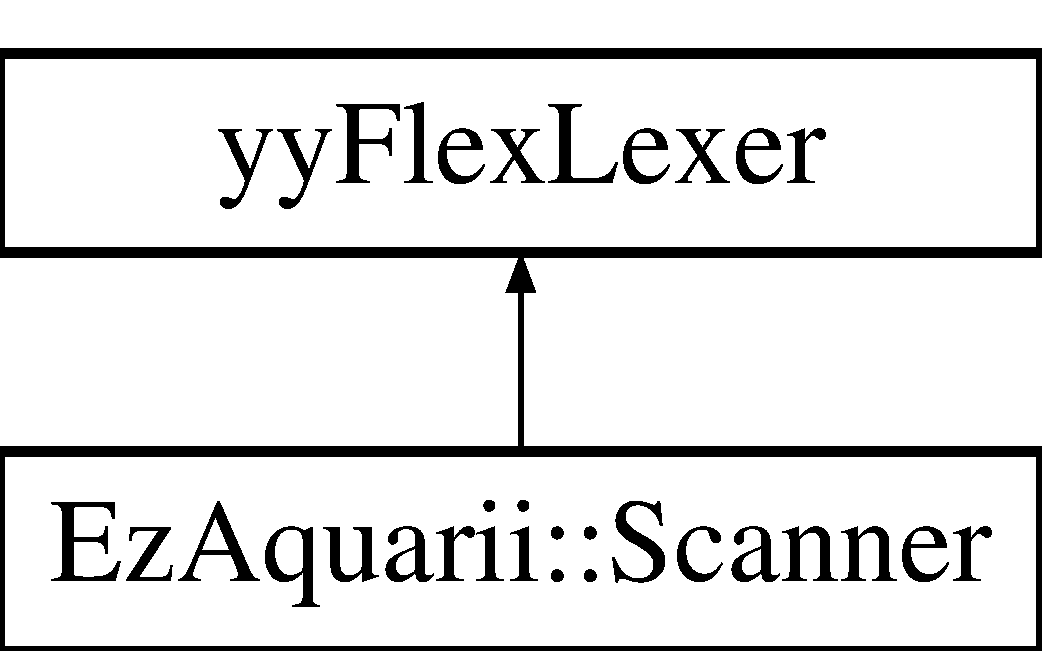
\includegraphics[height=2.000000cm]{classEzAquarii_1_1Scanner}
\end{center}
\end{figure}
\subsection*{Public Member Functions}
\begin{DoxyCompactItemize}
\item 
{\bfseries Scanner} (\hyperlink{classEzAquarii_1_1Interpreter}{Interpreter} \&driver)\hypertarget{classEzAquarii_1_1Scanner_ac9e5d9ea1525e795669228e37d9e33c6}{}\label{classEzAquarii_1_1Scanner_ac9e5d9ea1525e795669228e37d9e33c6}

\item 
virtual \hyperlink{classEzAquarii_1_1Parser_a219e44a6cf61b8a88cf0db8d5bb7be5d}{Ez\+Aquarii\+::\+Parser\+::symbol\+\_\+type} {\bfseries get\+\_\+next\+\_\+token} ()\hypertarget{classEzAquarii_1_1Scanner_aa90a8f3bdbdee9301d9e155be3238f2d}{}\label{classEzAquarii_1_1Scanner_aa90a8f3bdbdee9301d9e155be3238f2d}

\end{DoxyCompactItemize}


The documentation for this class was generated from the following file\+:\begin{DoxyCompactItemize}
\item 
/home/mate/\+Documents/\+Programming/\+Research/\+Multilayer\+Network\+Model/\+Multilayer\+Network\+Model/src/parser/include/scanner.\+h\end{DoxyCompactItemize}

\hypertarget{classEzAquarii_1_1slice}{}\section{Ez\+Aquarii\+:\+:slice$<$ T, S $>$ Class Template Reference}
\label{classEzAquarii_1_1slice}\index{Ez\+Aquarii\+::slice$<$ T, S $>$@{Ez\+Aquarii\+::slice$<$ T, S $>$}}


Present a slice of the top of a stack.  




{\ttfamily \#include $<$stack.\+hh$>$}

\subsection*{Public Member Functions}
\begin{DoxyCompactItemize}
\item 
{\bfseries slice} (const S \&\hyperlink{classEzAquarii_1_1stack}{stack}, unsigned int range)\hypertarget{classEzAquarii_1_1slice_a90d7a60ac36593984754dee9129a0a66}{}\label{classEzAquarii_1_1slice_a90d7a60ac36593984754dee9129a0a66}

\item 
const T \& {\bfseries operator\mbox{[}$\,$\mbox{]}} (unsigned int i) const \hypertarget{classEzAquarii_1_1slice_a4f1d600ec9aa96b82c70ce8af576ab74}{}\label{classEzAquarii_1_1slice_a4f1d600ec9aa96b82c70ce8af576ab74}

\end{DoxyCompactItemize}


\subsection{Detailed Description}
\subsubsection*{template$<$class T, class S = stack$<$\+T$>$$>$\\*
class Ez\+Aquarii\+::slice$<$ T, S $>$}

Present a slice of the top of a stack. 

The documentation for this class was generated from the following file\+:\begin{DoxyCompactItemize}
\item 
/home/mate/\+Documents/\+Programming/\+Research/\+Multilayer\+Network\+Model/\+Multilayer\+Network\+Model/src/parser/include/\hyperlink{stack_8hh}{stack.\+hh}\end{DoxyCompactItemize}

\hypertarget{classEzAquarii_1_1stack}{}\section{Ez\+Aquarii\+:\+:stack$<$ T, S $>$ Class Template Reference}
\label{classEzAquarii_1_1stack}\index{Ez\+Aquarii\+::stack$<$ T, S $>$@{Ez\+Aquarii\+::stack$<$ T, S $>$}}
\subsection*{Public Types}
\begin{DoxyCompactItemize}
\item 
typedef S\+::reverse\+\_\+iterator {\bfseries iterator}\hypertarget{classEzAquarii_1_1stack_aa90f54234fa3f44aa76455a034f67545}{}\label{classEzAquarii_1_1stack_aa90f54234fa3f44aa76455a034f67545}

\item 
typedef S\+::const\+\_\+reverse\+\_\+iterator {\bfseries const\+\_\+iterator}\hypertarget{classEzAquarii_1_1stack_a9c04a7fcb47dc3c07f9ad12d1fc554cf}{}\label{classEzAquarii_1_1stack_a9c04a7fcb47dc3c07f9ad12d1fc554cf}

\end{DoxyCompactItemize}
\subsection*{Public Member Functions}
\begin{DoxyCompactItemize}
\item 
{\bfseries stack} (unsigned int n)\hypertarget{classEzAquarii_1_1stack_a1279c5b5db10a39046b0057a3146ad08}{}\label{classEzAquarii_1_1stack_a1279c5b5db10a39046b0057a3146ad08}

\item 
T \& {\bfseries operator\mbox{[}$\,$\mbox{]}} (unsigned int i)\hypertarget{classEzAquarii_1_1stack_a94fbf24df24c2b63580973a33c4774ab}{}\label{classEzAquarii_1_1stack_a94fbf24df24c2b63580973a33c4774ab}

\item 
const T \& {\bfseries operator\mbox{[}$\,$\mbox{]}} (unsigned int i) const \hypertarget{classEzAquarii_1_1stack_ae4f90ae16e8cf89a38f17727d0350790}{}\label{classEzAquarii_1_1stack_ae4f90ae16e8cf89a38f17727d0350790}

\item 
void \hyperlink{classEzAquarii_1_1stack_adf8eeda90efd761b757bc3fb10a322f2}{push} (T \&t)
\item 
void {\bfseries pop} (unsigned int n=1)\hypertarget{classEzAquarii_1_1stack_a0d83764724c1aeb0866bea4283ca949a}{}\label{classEzAquarii_1_1stack_a0d83764724c1aeb0866bea4283ca949a}

\item 
void {\bfseries clear} ()\hypertarget{classEzAquarii_1_1stack_a4c3850ed1979fe0d53df99b9f30e87a4}{}\label{classEzAquarii_1_1stack_a4c3850ed1979fe0d53df99b9f30e87a4}

\item 
S\+::size\+\_\+type {\bfseries size} () const \hypertarget{classEzAquarii_1_1stack_a1701313d320e2d33d48b1bab7190feac}{}\label{classEzAquarii_1_1stack_a1701313d320e2d33d48b1bab7190feac}

\item 
const\+\_\+iterator {\bfseries begin} () const \hypertarget{classEzAquarii_1_1stack_a74d1ce60cc8058f0aebbad274e72e377}{}\label{classEzAquarii_1_1stack_a74d1ce60cc8058f0aebbad274e72e377}

\item 
const\+\_\+iterator {\bfseries end} () const \hypertarget{classEzAquarii_1_1stack_a798ca75fed270bf8467eafbc4833e829}{}\label{classEzAquarii_1_1stack_a798ca75fed270bf8467eafbc4833e829}

\end{DoxyCompactItemize}


\subsection{Member Function Documentation}
\index{Ez\+Aquarii\+::stack@{Ez\+Aquarii\+::stack}!push@{push}}
\index{push@{push}!Ez\+Aquarii\+::stack@{Ez\+Aquarii\+::stack}}
\subsubsection[{\texorpdfstring{push(\+T \&t)}{push(T &t)}}]{\setlength{\rightskip}{0pt plus 5cm}template$<$class T, class S = std\+::vector$<$\+T$>$$>$ void {\bf Ez\+Aquarii\+::stack}$<$ T, S $>$\+::push (
\begin{DoxyParamCaption}
\item[{T \&}]{t}
\end{DoxyParamCaption}
)\hspace{0.3cm}{\ttfamily [inline]}}\hypertarget{classEzAquarii_1_1stack_adf8eeda90efd761b757bc3fb10a322f2}{}\label{classEzAquarii_1_1stack_adf8eeda90efd761b757bc3fb10a322f2}
Steal the contents of {\itshape t}.

Close to move-\/semantics. 

The documentation for this class was generated from the following file\+:\begin{DoxyCompactItemize}
\item 
/home/mate/\+Documents/\+Programming/\+Research/\+Multilayer\+Network\+Model/\+Multilayer\+Network\+Model/src/parser/include/\hyperlink{stack_8hh}{stack.\+hh}\end{DoxyCompactItemize}

\hypertarget{classStructureGeneratorImpl}{}\section{Structure\+Generator\+Impl Class Reference}
\label{classStructureGeneratorImpl}\index{Structure\+Generator\+Impl@{Structure\+Generator\+Impl}}
Inheritance diagram for Structure\+Generator\+Impl\+:\begin{figure}[H]
\begin{center}
\leavevmode
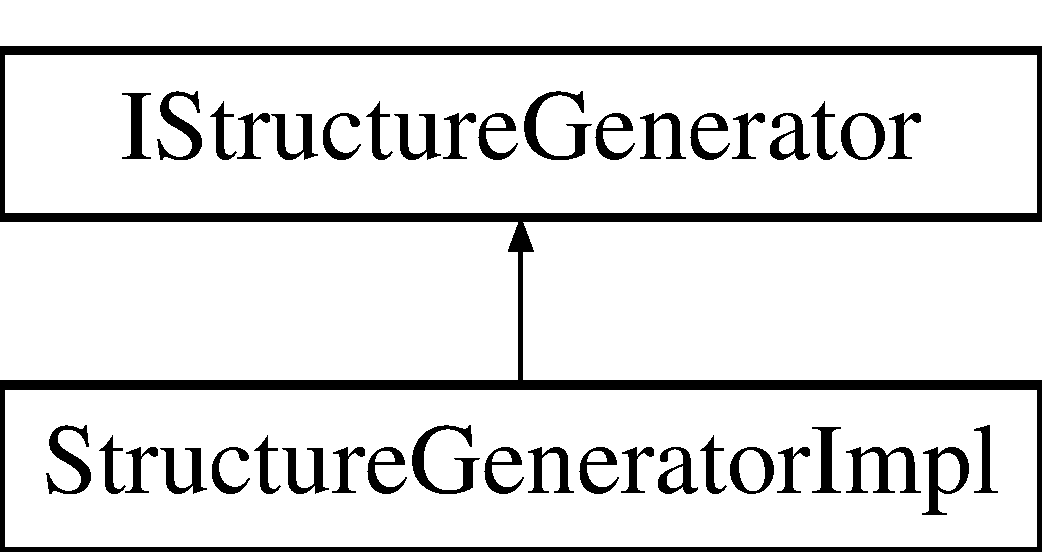
\includegraphics[height=2.000000cm]{classStructureGeneratorImpl}
\end{center}
\end{figure}
\subsection*{Public Member Functions}
\begin{DoxyCompactItemize}
\item 
{\bfseries Structure\+Generator\+Impl} (\hyperlink{classMultilayerNetwork}{Multilayer\+Network} $\ast$multilayer\+Network)\hypertarget{classStructureGeneratorImpl_a0e4efd8bc7d6f805054578026201ae38}{}\label{classStructureGeneratorImpl_a0e4efd8bc7d6f805054578026201ae38}

\item 
void {\bfseries generate\+Structure} ()\hypertarget{classStructureGeneratorImpl_a775184223dfef6f0e771589db2049993}{}\label{classStructureGeneratorImpl_a775184223dfef6f0e771589db2049993}

\end{DoxyCompactItemize}
\subsection*{Additional Inherited Members}


The documentation for this class was generated from the following files\+:\begin{DoxyCompactItemize}
\item 
/home/mate/\+Documents/\+Programming/\+Research/\+Multilayer\+Network\+Model/\+Multilayer\+Network\+Model/sources/generators/include/Structure\+Generator\+Impl.\+hh\item 
/home/mate/\+Documents/\+Programming/\+Research/\+Multilayer\+Network\+Model/\+Multilayer\+Network\+Model/sources/generators/src/Structure\+Generator\+Impl.\+cc\end{DoxyCompactItemize}

\hypertarget{structEzAquarii_1_1Parser_1_1syntax__error}{}\section{Ez\+Aquarii\+:\+:Parser\+:\+:syntax\+\_\+error Struct Reference}
\label{structEzAquarii_1_1Parser_1_1syntax__error}\index{Ez\+Aquarii\+::\+Parser\+::syntax\+\_\+error@{Ez\+Aquarii\+::\+Parser\+::syntax\+\_\+error}}


Syntax errors thrown from user actions.  




{\ttfamily \#include $<$parser.\+hpp$>$}

Inheritance diagram for Ez\+Aquarii\+:\+:Parser\+:\+:syntax\+\_\+error\+:\begin{figure}[H]
\begin{center}
\leavevmode
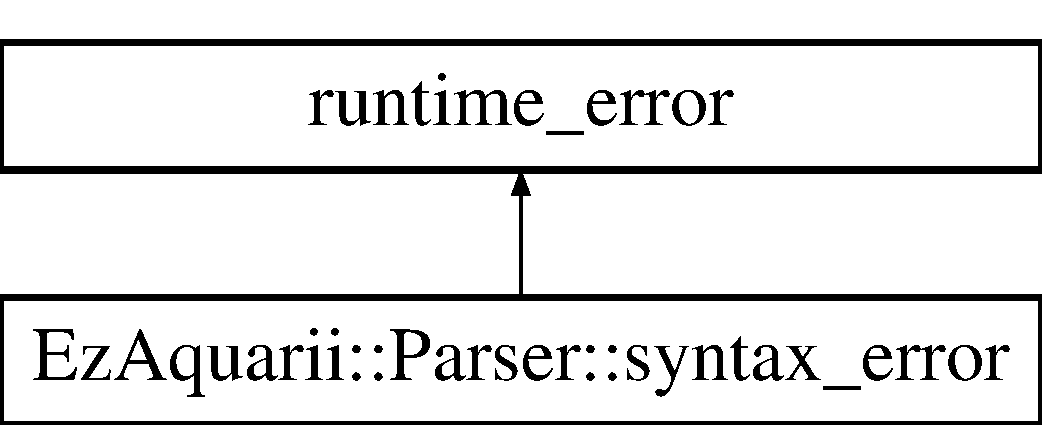
\includegraphics[height=2.000000cm]{structEzAquarii_1_1Parser_1_1syntax__error}
\end{center}
\end{figure}
\subsection*{Public Member Functions}
\begin{DoxyCompactItemize}
\item 
{\bfseries syntax\+\_\+error} (const \hyperlink{classEzAquarii_1_1Parser_acc4b937a827f1be285bf28ec90eeb125}{location\+\_\+type} \&l, const std\+::string \&m)\hypertarget{structEzAquarii_1_1Parser_1_1syntax__error_ad0c4657702d3609ecead4372137a7fe4}{}\label{structEzAquarii_1_1Parser_1_1syntax__error_ad0c4657702d3609ecead4372137a7fe4}

\end{DoxyCompactItemize}
\subsection*{Public Attributes}
\begin{DoxyCompactItemize}
\item 
\hyperlink{classEzAquarii_1_1Parser_acc4b937a827f1be285bf28ec90eeb125}{location\+\_\+type} {\bfseries location}\hypertarget{structEzAquarii_1_1Parser_1_1syntax__error_a7f8386ad39e13d5c883c920400e00d2d}{}\label{structEzAquarii_1_1Parser_1_1syntax__error_a7f8386ad39e13d5c883c920400e00d2d}

\end{DoxyCompactItemize}


\subsection{Detailed Description}
Syntax errors thrown from user actions. 

The documentation for this struct was generated from the following file\+:\begin{DoxyCompactItemize}
\item 
/home/mate/\+Documents/\+Programming/\+Research/\+Multilayer\+Network\+Model/\+Multilayer\+Network\+Model/src/parser/include/\hyperlink{parser_8hpp}{parser.\+hpp}\end{DoxyCompactItemize}

\hypertarget{structEzAquarii_1_1Parser_1_1token}{}\section{Ez\+Aquarii\+:\+:Parser\+:\+:token Struct Reference}
\label{structEzAquarii_1_1Parser_1_1token}\index{Ez\+Aquarii\+::\+Parser\+::token@{Ez\+Aquarii\+::\+Parser\+::token}}


Tokens.  




{\ttfamily \#include $<$parser.\+hpp$>$}

\subsection*{Public Types}
\begin{DoxyCompactItemize}
\item 
enum {\bfseries yytokentype} \{ \\*
{\bfseries T\+O\+K\+E\+N\+\_\+\+E\+ND} = 0, 
{\bfseries T\+O\+K\+E\+N\+\_\+\+S\+T\+R\+I\+NG} = 258, 
{\bfseries T\+O\+K\+E\+N\+\_\+\+L\+E\+F\+T\+P\+AR} = 259, 
{\bfseries T\+O\+K\+E\+N\+\_\+\+R\+I\+G\+H\+T\+P\+AR} = 260, 
\\*
{\bfseries T\+O\+K\+E\+N\+\_\+\+S\+E\+M\+I\+C\+O\+L\+ON} = 261, 
{\bfseries T\+O\+K\+E\+N\+\_\+\+C\+O\+M\+MA} = 262, 
{\bfseries T\+O\+K\+E\+N\+\_\+\+I\+N\+T\+E\+G\+ER} = 263, 
{\bfseries T\+O\+K\+E\+N\+\_\+\+D\+O\+U\+B\+LE} = 264, 
\\*
{\bfseries T\+O\+K\+E\+N\+\_\+\+P\+L\+US} = 265, 
{\bfseries T\+O\+K\+E\+N\+\_\+\+M\+I\+N\+US} = 266, 
{\bfseries T\+O\+K\+E\+N\+\_\+\+M\+U\+L\+T\+I\+P\+LY} = 267, 
{\bfseries T\+O\+K\+E\+N\+\_\+\+D\+I\+V\+I\+DE} = 268, 
\\*
{\bfseries T\+O\+K\+E\+N\+\_\+\+P\+O\+W\+ER} = 269
 \}\hypertarget{structEzAquarii_1_1Parser_1_1token_a2411b5b5510736b3c5e578685bf95fe1}{}\label{structEzAquarii_1_1Parser_1_1token_a2411b5b5510736b3c5e578685bf95fe1}

\end{DoxyCompactItemize}


\subsection{Detailed Description}
Tokens. 

The documentation for this struct was generated from the following file\+:\begin{DoxyCompactItemize}
\item 
/home/mate/\+Documents/\+Programming/\+Research/\+Multilayer\+Network\+Model/\+Multilayer\+Network\+Model/src/parser/include/\hyperlink{parser_8hpp}{parser.\+hpp}\end{DoxyCompactItemize}

\hypertarget{unionEzAquarii_1_1Parser_1_1union__type}{}\section{Ez\+Aquarii\+:\+:Parser\+:\+:union\+\_\+type Union Reference}
\label{unionEzAquarii_1_1Parser_1_1union__type}\index{Ez\+Aquarii\+::\+Parser\+::union\+\_\+type@{Ez\+Aquarii\+::\+Parser\+::union\+\_\+type}}


An auxiliary type to compute the largest semantic type.  




{\ttfamily \#include $<$parser.\+hpp$>$}

\subsection*{Public Attributes}
\begin{DoxyCompactItemize}
\item 
char {\bfseries dummy1} \mbox{[}sizeof(class \hyperlink{classCalculationNode}{Calculation\+Node} $\ast$)\mbox{]}\hypertarget{unionEzAquarii_1_1Parser_1_1union__type_a8dc1c487beaaea42f7e707e6b58fe558}{}\label{unionEzAquarii_1_1Parser_1_1union__type_a8dc1c487beaaea42f7e707e6b58fe558}

\item 
char {\bfseries dummy2} \mbox{[}sizeof(double)\mbox{]}\hypertarget{unionEzAquarii_1_1Parser_1_1union__type_a7f2c4f1d701cacda3f26062a6078608e}{}\label{unionEzAquarii_1_1Parser_1_1union__type_a7f2c4f1d701cacda3f26062a6078608e}

\item 
char {\bfseries dummy3} \mbox{[}sizeof(int)\mbox{]}\hypertarget{unionEzAquarii_1_1Parser_1_1union__type_ad046a9b9880ea1f74733ee8010dfdabe}{}\label{unionEzAquarii_1_1Parser_1_1union__type_ad046a9b9880ea1f74733ee8010dfdabe}

\item 
char {\bfseries dummy4} \mbox{[}sizeof(std\+::string)\mbox{]}\hypertarget{unionEzAquarii_1_1Parser_1_1union__type_a3be232be35298c96ff84e73bd6cf931e}{}\label{unionEzAquarii_1_1Parser_1_1union__type_a3be232be35298c96ff84e73bd6cf931e}

\end{DoxyCompactItemize}


\subsection{Detailed Description}
An auxiliary type to compute the largest semantic type. 

The documentation for this union was generated from the following file\+:\begin{DoxyCompactItemize}
\item 
/home/mate/\+Documents/\+Programming/\+Research/\+Multilayer\+Network\+Model/\+Multilayer\+Network\+Model/src/parser/include/\hyperlink{parser_8hpp}{parser.\+hpp}\end{DoxyCompactItemize}

\hypertarget{classUpwardInfluenceImpl}{}\section{Upward\+Influence\+Impl Class Reference}
\label{classUpwardInfluenceImpl}\index{Upward\+Influence\+Impl@{Upward\+Influence\+Impl}}
Inheritance diagram for Upward\+Influence\+Impl\+:\begin{figure}[H]
\begin{center}
\leavevmode
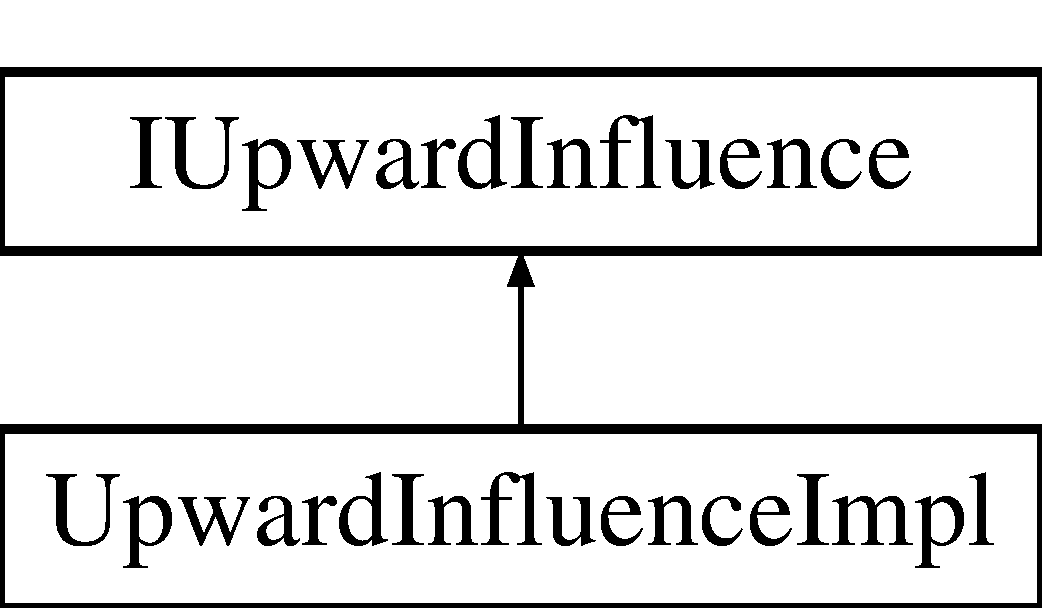
\includegraphics[height=2.000000cm]{classUpwardInfluenceImpl}
\end{center}
\end{figure}
\subsection*{Public Member Functions}
\begin{DoxyCompactItemize}
\item 
{\bfseries Upward\+Influence\+Impl} (\hyperlink{classNode}{Node} $\ast$node)\hypertarget{classUpwardInfluenceImpl_a33c1dc6e1d3cd99e7fab6c9cbc797fcf}{}\label{classUpwardInfluenceImpl_a33c1dc6e1d3cd99e7fab6c9cbc797fcf}

\item 
void {\bfseries calculate\+Upward\+Influence} ()\hypertarget{classUpwardInfluenceImpl_a30b4639db2644244553b54300f84a12c}{}\label{classUpwardInfluenceImpl_a30b4639db2644244553b54300f84a12c}

\end{DoxyCompactItemize}
\subsection*{Additional Inherited Members}


The documentation for this class was generated from the following files\+:\begin{DoxyCompactItemize}
\item 
/home/mate/\+Documents/\+Programming/\+Research/\+Multilayer\+Network\+Model/\+Multilayer\+Network\+Model/src/core/include/Upward\+Influence\+Impl.\+hh\item 
/home/mate/\+Documents/\+Programming/\+Research/\+Multilayer\+Network\+Model/\+Multilayer\+Network\+Model/src/core/src/Upward\+Influence\+Impl.\+cc\end{DoxyCompactItemize}

\hypertarget{structEzAquarii_1_1variant}{}\section{Ez\+Aquarii\+:\+:variant$<$ S $>$ Struct Template Reference}
\label{structEzAquarii_1_1variant}\index{Ez\+Aquarii\+::variant$<$ S $>$@{Ez\+Aquarii\+::variant$<$ S $>$}}


{\ttfamily \#include $<$parser.\+hpp$>$}

\subsection*{Public Types}
\begin{DoxyCompactItemize}
\item 
typedef \hyperlink{structEzAquarii_1_1variant}{variant}$<$ S $>$ \hyperlink{structEzAquarii_1_1variant_af94dbfa9a3e7310b9827d20cc65163a8}{self\+\_\+type}\hypertarget{structEzAquarii_1_1variant_af94dbfa9a3e7310b9827d20cc65163a8}{}\label{structEzAquarii_1_1variant_af94dbfa9a3e7310b9827d20cc65163a8}

\begin{DoxyCompactList}\small\item\em Type of $\ast$this. \end{DoxyCompactList}\end{DoxyCompactItemize}
\subsection*{Public Member Functions}
\begin{DoxyCompactItemize}
\item 
\hyperlink{structEzAquarii_1_1variant_aba217414b27084fcfe62cc3e5e4b6e1f}{variant} ()\hypertarget{structEzAquarii_1_1variant_aba217414b27084fcfe62cc3e5e4b6e1f}{}\label{structEzAquarii_1_1variant_aba217414b27084fcfe62cc3e5e4b6e1f}

\begin{DoxyCompactList}\small\item\em Empty construction. \end{DoxyCompactList}\item 
{\footnotesize template$<$typename T $>$ }\\\hyperlink{structEzAquarii_1_1variant_a7aa6d2d6ef84300ce6058386da4fd301}{variant} (const T \&t)\hypertarget{structEzAquarii_1_1variant_a7aa6d2d6ef84300ce6058386da4fd301}{}\label{structEzAquarii_1_1variant_a7aa6d2d6ef84300ce6058386da4fd301}

\begin{DoxyCompactList}\small\item\em Construct and fill. \end{DoxyCompactList}\item 
\hyperlink{structEzAquarii_1_1variant_ada4ce2e2f8d43d1628b5512d8d142d79}{$\sim$variant} ()\hypertarget{structEzAquarii_1_1variant_ada4ce2e2f8d43d1628b5512d8d142d79}{}\label{structEzAquarii_1_1variant_ada4ce2e2f8d43d1628b5512d8d142d79}

\begin{DoxyCompactList}\small\item\em Destruction, allowed only if empty. \end{DoxyCompactList}\item 
{\footnotesize template$<$typename T $>$ }\\T \& \hyperlink{structEzAquarii_1_1variant_a47da404b9eee848de509436cec5b4867}{build} ()\hypertarget{structEzAquarii_1_1variant_a47da404b9eee848de509436cec5b4867}{}\label{structEzAquarii_1_1variant_a47da404b9eee848de509436cec5b4867}

\begin{DoxyCompactList}\small\item\em Instantiate an empty {\itshape T} in here. \end{DoxyCompactList}\item 
{\footnotesize template$<$typename T $>$ }\\T \& \hyperlink{structEzAquarii_1_1variant_aa60ced10dbe65260b88d83c02b728a9b}{build} (const T \&t)\hypertarget{structEzAquarii_1_1variant_aa60ced10dbe65260b88d83c02b728a9b}{}\label{structEzAquarii_1_1variant_aa60ced10dbe65260b88d83c02b728a9b}

\begin{DoxyCompactList}\small\item\em Instantiate a {\itshape T} in here from {\itshape t}. \end{DoxyCompactList}\item 
{\footnotesize template$<$typename T $>$ }\\T \& \hyperlink{structEzAquarii_1_1variant_a47128db59e96b94a6e9ccda7c5a64ba7}{as} ()\hypertarget{structEzAquarii_1_1variant_a47128db59e96b94a6e9ccda7c5a64ba7}{}\label{structEzAquarii_1_1variant_a47128db59e96b94a6e9ccda7c5a64ba7}

\begin{DoxyCompactList}\small\item\em Accessor to a built {\itshape T}. \end{DoxyCompactList}\item 
{\footnotesize template$<$typename T $>$ }\\const T \& \hyperlink{structEzAquarii_1_1variant_ad3acf50de2a0c3cc09e97f818f9cfa3f}{as} () const \hypertarget{structEzAquarii_1_1variant_ad3acf50de2a0c3cc09e97f818f9cfa3f}{}\label{structEzAquarii_1_1variant_ad3acf50de2a0c3cc09e97f818f9cfa3f}

\begin{DoxyCompactList}\small\item\em Const accessor to a built {\itshape T} (for printer). \end{DoxyCompactList}\item 
{\footnotesize template$<$typename T $>$ }\\void \hyperlink{structEzAquarii_1_1variant_a13e5d2c240938d776079a84a4d0a2885}{swap} (\hyperlink{structEzAquarii_1_1variant_af94dbfa9a3e7310b9827d20cc65163a8}{self\+\_\+type} \&other)
\item 
{\footnotesize template$<$typename T $>$ }\\void \hyperlink{structEzAquarii_1_1variant_aa40237e6c2cdf568f8098defd28ecbc7}{move} (\hyperlink{structEzAquarii_1_1variant_af94dbfa9a3e7310b9827d20cc65163a8}{self\+\_\+type} \&other)
\item 
{\footnotesize template$<$typename T $>$ }\\void \hyperlink{structEzAquarii_1_1variant_a22bc1304b6bcc561fbb09fe4ee65da40}{copy} (const \hyperlink{structEzAquarii_1_1variant_af94dbfa9a3e7310b9827d20cc65163a8}{self\+\_\+type} \&other)\hypertarget{structEzAquarii_1_1variant_a22bc1304b6bcc561fbb09fe4ee65da40}{}\label{structEzAquarii_1_1variant_a22bc1304b6bcc561fbb09fe4ee65da40}

\begin{DoxyCompactList}\small\item\em Copy the content of {\itshape other} to this. \end{DoxyCompactList}\item 
{\footnotesize template$<$typename T $>$ }\\void \hyperlink{structEzAquarii_1_1variant_a1b38a5712514f1165364b4245f57429f}{destroy} ()\hypertarget{structEzAquarii_1_1variant_a1b38a5712514f1165364b4245f57429f}{}\label{structEzAquarii_1_1variant_a1b38a5712514f1165364b4245f57429f}

\begin{DoxyCompactList}\small\item\em Destroy the stored {\itshape T}. \end{DoxyCompactList}\end{DoxyCompactItemize}


\subsection{Detailed Description}
\subsubsection*{template$<$size\+\_\+t S$>$\\*
struct Ez\+Aquarii\+::variant$<$ S $>$}

A char\mbox{[}S\mbox{]} buffer to store and retrieve objects.

Sort of a variant, but does not keep track of the nature of the stored data, since that knowledge is available via the current state. 

\subsection{Member Function Documentation}
\index{Ez\+Aquarii\+::variant@{Ez\+Aquarii\+::variant}!move@{move}}
\index{move@{move}!Ez\+Aquarii\+::variant@{Ez\+Aquarii\+::variant}}
\subsubsection[{\texorpdfstring{move(self\+\_\+type \&other)}{move(self_type &other)}}]{\setlength{\rightskip}{0pt plus 5cm}template$<$size\+\_\+t S$>$ template$<$typename T $>$ void {\bf Ez\+Aquarii\+::variant}$<$ S $>$\+::move (
\begin{DoxyParamCaption}
\item[{{\bf self\+\_\+type} \&}]{other}
\end{DoxyParamCaption}
)\hspace{0.3cm}{\ttfamily [inline]}}\hypertarget{structEzAquarii_1_1variant_aa40237e6c2cdf568f8098defd28ecbc7}{}\label{structEzAquarii_1_1variant_aa40237e6c2cdf568f8098defd28ecbc7}
Move the content of {\itshape other} to this.

Destroys {\itshape other}. \index{Ez\+Aquarii\+::variant@{Ez\+Aquarii\+::variant}!swap@{swap}}
\index{swap@{swap}!Ez\+Aquarii\+::variant@{Ez\+Aquarii\+::variant}}
\subsubsection[{\texorpdfstring{swap(self\+\_\+type \&other)}{swap(self_type &other)}}]{\setlength{\rightskip}{0pt plus 5cm}template$<$size\+\_\+t S$>$ template$<$typename T $>$ void {\bf Ez\+Aquarii\+::variant}$<$ S $>$\+::swap (
\begin{DoxyParamCaption}
\item[{{\bf self\+\_\+type} \&}]{other}
\end{DoxyParamCaption}
)\hspace{0.3cm}{\ttfamily [inline]}}\hypertarget{structEzAquarii_1_1variant_a13e5d2c240938d776079a84a4d0a2885}{}\label{structEzAquarii_1_1variant_a13e5d2c240938d776079a84a4d0a2885}
Swap the content with {\itshape other}, of same type.

Both variants must be built beforehand, because swapping the actual data requires reading it (with \hyperlink{structEzAquarii_1_1variant_a47128db59e96b94a6e9ccda7c5a64ba7}{as()}), and this is not possible on unconstructed variants\+: it would require some dynamic testing, which should not be the variant\textquotesingle{}s responsability. Swapping between built and (possibly) non-\/built is done with \hyperlink{structEzAquarii_1_1variant_aa40237e6c2cdf568f8098defd28ecbc7}{variant\+::move} (). 

The documentation for this struct was generated from the following file\+:\begin{DoxyCompactItemize}
\item 
/home/mate/\+Documents/\+Programming/\+Research/\+Multilayer\+Network\+Model/\+Multilayer\+Network\+Model/src/parser/include/\hyperlink{parser_8hpp}{parser.\+hpp}\end{DoxyCompactItemize}

\hypertarget{classVectorField}{}\section{Vector\+Field Class Reference}
\label{classVectorField}\index{Vector\+Field@{Vector\+Field}}
\subsection*{Public Member Functions}
\begin{DoxyCompactItemize}
\item 
void {\bfseries add\+Point} (std\+::map$<$ int, double $>$ coordinate, std\+::map$<$ int, double $>$ direction)\hypertarget{classVectorField_ac72253d7b3410d3ef4ea520fded2d1f1}{}\label{classVectorField_ac72253d7b3410d3ef4ea520fded2d1f1}

\item 
std\+::vector$<$ \hyperlink{classVectorFieldPoint}{Vector\+Field\+Point} $\ast$ $>$ {\bfseries get\+Vector\+Field\+Points} ()\hypertarget{classVectorField_a79f35e239c04f89a3987f8ae70b49ef9}{}\label{classVectorField_a79f35e239c04f89a3987f8ae70b49ef9}

\item 
double {\bfseries get\+Distance\+From} (\hyperlink{classVectorField}{Vector\+Field} $\ast$vector\+Field)\hypertarget{classVectorField_a9cf9f0a60b62422a406a8530e10ed402}{}\label{classVectorField_a9cf9f0a60b62422a406a8530e10ed402}

\item 
std\+::map$<$ int, double $>$ {\bfseries get\+Direction\+For\+Coordinate} (std\+::map$<$ int, double $>$ coordinate)\hypertarget{classVectorField_ae8f028240c6b4ba60815660a887b92a4}{}\label{classVectorField_ae8f028240c6b4ba60815660a887b92a4}

\end{DoxyCompactItemize}
\subsection*{Friends}
\begin{DoxyCompactItemize}
\item 
std\+::ostream \& {\bfseries operator$<$$<$} (std\+::ostream \&os, const \hyperlink{classVectorField}{Vector\+Field} \&vector\+Field)\hypertarget{classVectorField_a305be31f220fc6801fa91592e7a08a9b}{}\label{classVectorField_a305be31f220fc6801fa91592e7a08a9b}

\end{DoxyCompactItemize}


The documentation for this class was generated from the following files\+:\begin{DoxyCompactItemize}
\item 
/home/mate/\+Documents/\+Programming/\+Research/\+Multilayer\+Network\+Model/\+Multilayer\+Network\+Model/src/core/include/Vector\+Field.\+hh\item 
/home/mate/\+Documents/\+Programming/\+Research/\+Multilayer\+Network\+Model/\+Multilayer\+Network\+Model/src/core/src/Vector\+Field.\+cc\end{DoxyCompactItemize}

\hypertarget{classVectorFieldPoint}{}\section{Vector\+Field\+Point Class Reference}
\label{classVectorFieldPoint}\index{Vector\+Field\+Point@{Vector\+Field\+Point}}
\subsection*{Public Member Functions}
\begin{DoxyCompactItemize}
\item 
{\bfseries Vector\+Field\+Point} (std\+::map$<$ int, double $>$ coordinate, std\+::map$<$ int, double $>$ direction)\hypertarget{classVectorFieldPoint_aaf7f444221b412f58e3066fb359f6ced}{}\label{classVectorFieldPoint_aaf7f444221b412f58e3066fb359f6ced}

\item 
std\+::map$<$ int, double $>$ {\bfseries get\+Coordinate} ()\hypertarget{classVectorFieldPoint_aaac572daff42e5aa46d92ffc2f681095}{}\label{classVectorFieldPoint_aaac572daff42e5aa46d92ffc2f681095}

\item 
std\+::map$<$ int, double $>$ {\bfseries get\+Direction} ()\hypertarget{classVectorFieldPoint_a185b994999d47371fad7e8156e211f28}{}\label{classVectorFieldPoint_a185b994999d47371fad7e8156e211f28}

\end{DoxyCompactItemize}
\subsection*{Friends}
\begin{DoxyCompactItemize}
\item 
std\+::ostream \& {\bfseries operator$<$$<$} (std\+::ostream \&os, const \hyperlink{classVectorFieldPoint}{Vector\+Field\+Point} \&vector\+Field\+Point)\hypertarget{classVectorFieldPoint_a0acdca72efec81baafb8b278ed2a545f}{}\label{classVectorFieldPoint_a0acdca72efec81baafb8b278ed2a545f}

\end{DoxyCompactItemize}


The documentation for this class was generated from the following file\+:\begin{DoxyCompactItemize}
\item 
/home/mate/\+Documents/\+Programming/\+Research/\+Multilayer\+Network\+Model/\+Multilayer\+Network\+Model/sources/core/\+Vector\+Field\+Reconfiguration/include/Vector\+Field\+Point.\+hh\end{DoxyCompactItemize}

\hypertarget{classVectorFieldReconfigurationImpl}{}\section{Vector\+Field\+Reconfiguration\+Impl Class Reference}
\label{classVectorFieldReconfigurationImpl}\index{Vector\+Field\+Reconfiguration\+Impl@{Vector\+Field\+Reconfiguration\+Impl}}
Inheritance diagram for Vector\+Field\+Reconfiguration\+Impl\+:\begin{figure}[H]
\begin{center}
\leavevmode
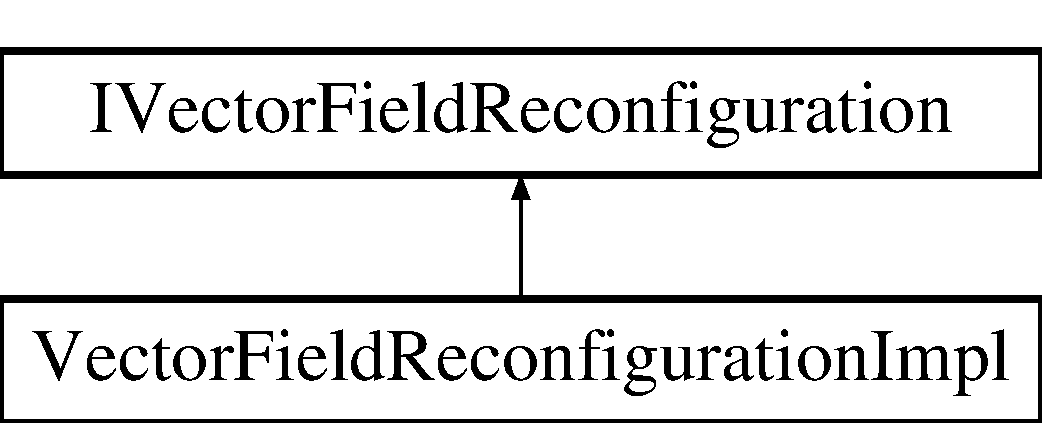
\includegraphics[height=2.000000cm]{classVectorFieldReconfigurationImpl}
\end{center}
\end{figure}
\subsection*{Public Member Functions}
\begin{DoxyCompactItemize}
\item 
{\bfseries Vector\+Field\+Reconfiguration\+Impl} (\hyperlink{classNode}{Node} $\ast$node)\hypertarget{classVectorFieldReconfigurationImpl_a42670d176dfc295f342033869defc178}{}\label{classVectorFieldReconfigurationImpl_a42670d176dfc295f342033869defc178}

\item 
void {\bfseries calculate\+Vector\+Field\+Reconfiguration} ()\hypertarget{classVectorFieldReconfigurationImpl_a2143e9fc6631fb61390e8881404891a5}{}\label{classVectorFieldReconfigurationImpl_a2143e9fc6631fb61390e8881404891a5}

\item 
void {\bfseries calculate\+Target\+Vector\+Field} (\hyperlink{classVectorField}{Vector\+Field} $\ast$target\+Vector\+Field, \hyperlink{classVectorField}{Vector\+Field} $\ast$current\+Vector\+Field, std\+::map$<$ int, double $>$ direction\+In\+Lower\+Network, std\+::map$<$ int, double $>$ direction\+In\+Higher\+Networks)\hypertarget{classVectorFieldReconfigurationImpl_aae26dcd63e8c68cfac045b90e101c522}{}\label{classVectorFieldReconfigurationImpl_aae26dcd63e8c68cfac045b90e101c522}

\item 
std\+::map$<$ int, double $>$ {\bfseries calculate\+Lower\+Network\+Direction} ()\hypertarget{classVectorFieldReconfigurationImpl_ab2746d147258dc03cf7ffbbfb0abe738}{}\label{classVectorFieldReconfigurationImpl_ab2746d147258dc03cf7ffbbfb0abe738}

\item 
std\+::map$<$ int, double $>$ {\bfseries calculate\+Higher\+Networks\+Direction} ()\hypertarget{classVectorFieldReconfigurationImpl_a2e6d7b501b830cfdbf069f8b70a75a62}{}\label{classVectorFieldReconfigurationImpl_a2e6d7b501b830cfdbf069f8b70a75a62}

\end{DoxyCompactItemize}
\subsection*{Additional Inherited Members}


The documentation for this class was generated from the following files\+:\begin{DoxyCompactItemize}
\item 
/home/mate/\+Documents/\+Programming/\+Research/\+Multilayer\+Network\+Model/\+Multilayer\+Network\+Model/src/core/include/Vector\+Field\+Reconfiguration\+Impl.\+hh\item 
/home/mate/\+Documents/\+Programming/\+Research/\+Multilayer\+Network\+Model/\+Multilayer\+Network\+Model/src/core/src/Vector\+Field\+Reconfiguration\+Impl.\+cc\end{DoxyCompactItemize}

\hypertarget{structyy__buffer__state}{}\section{yy\+\_\+buffer\+\_\+state Struct Reference}
\label{structyy__buffer__state}\index{yy\+\_\+buffer\+\_\+state@{yy\+\_\+buffer\+\_\+state}}
\subsection*{Public Attributes}
\begin{DoxyCompactItemize}
\item 
std\+::istream $\ast$ {\bfseries yy\+\_\+input\+\_\+file}\hypertarget{structyy__buffer__state_a3cea2f85a5c18fae4a8dd1ca44c3a977}{}\label{structyy__buffer__state_a3cea2f85a5c18fae4a8dd1ca44c3a977}

\item 
char $\ast$ {\bfseries yy\+\_\+ch\+\_\+buf}\hypertarget{structyy__buffer__state_ad7b8df8d8a4688e57b0b8d3ca75adc85}{}\label{structyy__buffer__state_ad7b8df8d8a4688e57b0b8d3ca75adc85}

\item 
char $\ast$ {\bfseries yy\+\_\+buf\+\_\+pos}\hypertarget{structyy__buffer__state_a58aa927f098b99d99e75da80f9b681ef}{}\label{structyy__buffer__state_a58aa927f098b99d99e75da80f9b681ef}

\item 
int {\bfseries yy\+\_\+buf\+\_\+size}\hypertarget{structyy__buffer__state_a451d39697f006f3922c1f43cf79286b4}{}\label{structyy__buffer__state_a451d39697f006f3922c1f43cf79286b4}

\item 
int {\bfseries yy\+\_\+n\+\_\+chars}\hypertarget{structyy__buffer__state_a06406208824817acfec2183b79080945}{}\label{structyy__buffer__state_a06406208824817acfec2183b79080945}

\item 
int {\bfseries yy\+\_\+is\+\_\+our\+\_\+buffer}\hypertarget{structyy__buffer__state_a80ce2431c70dc4f89ced487f18449465}{}\label{structyy__buffer__state_a80ce2431c70dc4f89ced487f18449465}

\item 
int {\bfseries yy\+\_\+is\+\_\+interactive}\hypertarget{structyy__buffer__state_abf5c70eea75581b58c0ee7bd31b14490}{}\label{structyy__buffer__state_abf5c70eea75581b58c0ee7bd31b14490}

\item 
int {\bfseries yy\+\_\+at\+\_\+bol}\hypertarget{structyy__buffer__state_a9d60c60af6e1a6f69de16871fd64f85f}{}\label{structyy__buffer__state_a9d60c60af6e1a6f69de16871fd64f85f}

\item 
int \hyperlink{structyy__buffer__state_a818e94bc9c766e683c60df1e9fd01199}{yy\+\_\+bs\+\_\+lineno}
\item 
int \hyperlink{structyy__buffer__state_a10c4fcd8be759e6bf11e6d3e8cdb0307}{yy\+\_\+bs\+\_\+column}
\item 
int {\bfseries yy\+\_\+fill\+\_\+buffer}\hypertarget{structyy__buffer__state_a63d2afbb1d79a3fc63df9e12626f827d}{}\label{structyy__buffer__state_a63d2afbb1d79a3fc63df9e12626f827d}

\item 
int {\bfseries yy\+\_\+buffer\+\_\+status}\hypertarget{structyy__buffer__state_a70fd925d37a2f0454fbd0def675d106c}{}\label{structyy__buffer__state_a70fd925d37a2f0454fbd0def675d106c}

\end{DoxyCompactItemize}


\subsection{Member Data Documentation}
\index{yy\+\_\+buffer\+\_\+state@{yy\+\_\+buffer\+\_\+state}!yy\+\_\+bs\+\_\+column@{yy\+\_\+bs\+\_\+column}}
\index{yy\+\_\+bs\+\_\+column@{yy\+\_\+bs\+\_\+column}!yy\+\_\+buffer\+\_\+state@{yy\+\_\+buffer\+\_\+state}}
\subsubsection[{\texorpdfstring{yy\+\_\+bs\+\_\+column}{yy_bs_column}}]{\setlength{\rightskip}{0pt plus 5cm}int yy\+\_\+buffer\+\_\+state\+::yy\+\_\+bs\+\_\+column}\hypertarget{structyy__buffer__state_a10c4fcd8be759e6bf11e6d3e8cdb0307}{}\label{structyy__buffer__state_a10c4fcd8be759e6bf11e6d3e8cdb0307}
The column count. \index{yy\+\_\+buffer\+\_\+state@{yy\+\_\+buffer\+\_\+state}!yy\+\_\+bs\+\_\+lineno@{yy\+\_\+bs\+\_\+lineno}}
\index{yy\+\_\+bs\+\_\+lineno@{yy\+\_\+bs\+\_\+lineno}!yy\+\_\+buffer\+\_\+state@{yy\+\_\+buffer\+\_\+state}}
\subsubsection[{\texorpdfstring{yy\+\_\+bs\+\_\+lineno}{yy_bs_lineno}}]{\setlength{\rightskip}{0pt plus 5cm}int yy\+\_\+buffer\+\_\+state\+::yy\+\_\+bs\+\_\+lineno}\hypertarget{structyy__buffer__state_a818e94bc9c766e683c60df1e9fd01199}{}\label{structyy__buffer__state_a818e94bc9c766e683c60df1e9fd01199}
The line count. 

The documentation for this struct was generated from the following file\+:\begin{DoxyCompactItemize}
\item 
/home/mate/\+Documents/\+Programming/\+Research/\+Multilayer\+Network\+Model/\+Multilayer\+Network\+Model/src/parser/src/scanner.\+cpp\end{DoxyCompactItemize}

\hypertarget{structyy__trans__info}{}\section{yy\+\_\+trans\+\_\+info Struct Reference}
\label{structyy__trans__info}\index{yy\+\_\+trans\+\_\+info@{yy\+\_\+trans\+\_\+info}}
\subsection*{Public Attributes}
\begin{DoxyCompactItemize}
\item 
flex\+\_\+int32\+\_\+t {\bfseries yy\+\_\+verify}\hypertarget{structyy__trans__info_a5c9f61e770deef50bd4e697310342fe9}{}\label{structyy__trans__info_a5c9f61e770deef50bd4e697310342fe9}

\item 
flex\+\_\+int32\+\_\+t {\bfseries yy\+\_\+nxt}\hypertarget{structyy__trans__info_ae0715250c2bef261e596e77e0030f13e}{}\label{structyy__trans__info_ae0715250c2bef261e596e77e0030f13e}

\end{DoxyCompactItemize}


The documentation for this struct was generated from the following file\+:\begin{DoxyCompactItemize}
\item 
/home/mate/\+Documents/\+Programming/\+Research/\+Multilayer\+Network\+Model/\+Multilayer\+Network\+Model/src/parser/src/scanner.\+cpp\end{DoxyCompactItemize}

\chapter{File Documentation}
\hypertarget{location_8hh}{}\section{/home/mate/\+Documents/\+Programming/\+Research/\+Multilayer\+Network\+Model/\+Multilayer\+Network\+Model/src/parser/include/location.hh File Reference}
\label{location_8hh}\index{/home/mate/\+Documents/\+Programming/\+Research/\+Multilayer\+Network\+Model/\+Multilayer\+Network\+Model/src/parser/include/location.\+hh@{/home/mate/\+Documents/\+Programming/\+Research/\+Multilayer\+Network\+Model/\+Multilayer\+Network\+Model/src/parser/include/location.\+hh}}
{\ttfamily \#include \char`\"{}position.\+hh\char`\"{}}\\*
\subsection*{Classes}
\begin{DoxyCompactItemize}
\item 
class \hyperlink{classEquationParser_1_1location}{Equation\+Parser\+::location}
\begin{DoxyCompactList}\small\item\em Abstract a location. \end{DoxyCompactList}\end{DoxyCompactItemize}
\subsection*{Functions}
\begin{DoxyCompactItemize}
\item 
location \& \hyperlink{location_8hh_a857fd1b178de784f9a631c1268232e85}{Equation\+Parser\+::operator+=} (location \&res, const location \&end)\hypertarget{location_8hh_a857fd1b178de784f9a631c1268232e85}{}\label{location_8hh_a857fd1b178de784f9a631c1268232e85}

\begin{DoxyCompactList}\small\item\em Join two locations, in place. \end{DoxyCompactList}\item 
location \hyperlink{location_8hh_a2c17bf52a2f6f8c74da735c324ed71ea}{Equation\+Parser\+::operator+} (location res, const location \&end)\hypertarget{location_8hh_a2c17bf52a2f6f8c74da735c324ed71ea}{}\label{location_8hh_a2c17bf52a2f6f8c74da735c324ed71ea}

\begin{DoxyCompactList}\small\item\em Join two locations. \end{DoxyCompactList}\item 
location \& \hyperlink{location_8hh_a5a8ab2a400786124ef70e1403c1b16db}{Equation\+Parser\+::operator+=} (location \&res, int width)\hypertarget{location_8hh_a5a8ab2a400786124ef70e1403c1b16db}{}\label{location_8hh_a5a8ab2a400786124ef70e1403c1b16db}

\begin{DoxyCompactList}\small\item\em Add {\itshape width} columns to the end position, in place. \end{DoxyCompactList}\item 
location \hyperlink{location_8hh_a81130cb033ab2d03e8f3aee42233514e}{Equation\+Parser\+::operator+} (location res, int width)\hypertarget{location_8hh_a81130cb033ab2d03e8f3aee42233514e}{}\label{location_8hh_a81130cb033ab2d03e8f3aee42233514e}

\begin{DoxyCompactList}\small\item\em Add {\itshape width} columns to the end position. \end{DoxyCompactList}\item 
location \& \hyperlink{location_8hh_a623138b41508502b7217bb9d33aa7998}{Equation\+Parser\+::operator-\/=} (location \&res, int width)\hypertarget{location_8hh_a623138b41508502b7217bb9d33aa7998}{}\label{location_8hh_a623138b41508502b7217bb9d33aa7998}

\begin{DoxyCompactList}\small\item\em Subtract {\itshape width} columns to the end position, in place. \end{DoxyCompactList}\item 
location \hyperlink{location_8hh_a63a349232174befa3d2bb9ad28c776e7}{Equation\+Parser\+::operator-\/} (location res, int width)\hypertarget{location_8hh_a63a349232174befa3d2bb9ad28c776e7}{}\label{location_8hh_a63a349232174befa3d2bb9ad28c776e7}

\begin{DoxyCompactList}\small\item\em Subtract {\itshape width} columns to the end position. \end{DoxyCompactList}\item 
bool \hyperlink{location_8hh_ae6d0b523f7673c8da176a4c94e8278ae}{Equation\+Parser\+::operator==} (const location \&loc1, const location \&loc2)\hypertarget{location_8hh_ae6d0b523f7673c8da176a4c94e8278ae}{}\label{location_8hh_ae6d0b523f7673c8da176a4c94e8278ae}

\begin{DoxyCompactList}\small\item\em Compare two location objects. \end{DoxyCompactList}\item 
bool \hyperlink{location_8hh_a83d9eab30473390a2c1bd6c8d9e0161b}{Equation\+Parser\+::operator!=} (const location \&loc1, const location \&loc2)\hypertarget{location_8hh_a83d9eab30473390a2c1bd6c8d9e0161b}{}\label{location_8hh_a83d9eab30473390a2c1bd6c8d9e0161b}

\begin{DoxyCompactList}\small\item\em Compare two location objects. \end{DoxyCompactList}\item 
{\footnotesize template$<$typename Y\+Y\+Char $>$ }\\std\+::basic\+\_\+ostream$<$ Y\+Y\+Char $>$ \& \hyperlink{location_8hh_acad9fad3affdce34c0a30e675ce90753}{Equation\+Parser\+::operator$<$$<$} (std\+::basic\+\_\+ostream$<$ Y\+Y\+Char $>$ \&ostr, const location \&loc)
\begin{DoxyCompactList}\small\item\em Intercept output stream redirection. \end{DoxyCompactList}\end{DoxyCompactItemize}


\subsection{Detailed Description}
Define the Equation\+Parser \+::location class. 

\subsection{Function Documentation}
\index{location.\+hh@{location.\+hh}!operator$<$$<$@{operator$<$$<$}}
\index{operator$<$$<$@{operator$<$$<$}!location.\+hh@{location.\+hh}}
\subsubsection[{\texorpdfstring{operator$<$$<$(std\+::basic\+\_\+ostream$<$ Y\+Y\+Char $>$ \&ostr, const location \&loc)}{operator<<(std::basic_ostream< YYChar > &ostr, const location &loc)}}]{\setlength{\rightskip}{0pt plus 5cm}template$<$typename Y\+Y\+Char $>$ std\+::basic\+\_\+ostream$<$Y\+Y\+Char$>$\& Equation\+Parser\+::operator$<$$<$ (
\begin{DoxyParamCaption}
\item[{std\+::basic\+\_\+ostream$<$ Y\+Y\+Char $>$ \&}]{ostr, }
\item[{const {\bf location} \&}]{loc}
\end{DoxyParamCaption}
)\hspace{0.3cm}{\ttfamily [inline]}}\hypertarget{location_8hh_file_acad9fad3affdce34c0a30e675ce90753}{}\label{location_8hh_file_acad9fad3affdce34c0a30e675ce90753}


Intercept output stream redirection. 


\begin{DoxyParams}{Parameters}
{\em ostr} & the destination output stream \\
\hline
{\em loc} & a reference to the location to redirect\\
\hline
\end{DoxyParams}
Avoid duplicate information. 
\hypertarget{parser_8hpp}{}\section{/home/mate/\+Documents/\+Programming/\+Research/\+Multilayer\+Network\+Model/\+Multilayer\+Network\+Model/src/parser/include/parser.hpp File Reference}
\label{parser_8hpp}\index{/home/mate/\+Documents/\+Programming/\+Research/\+Multilayer\+Network\+Model/\+Multilayer\+Network\+Model/src/parser/include/parser.\+hpp@{/home/mate/\+Documents/\+Programming/\+Research/\+Multilayer\+Network\+Model/\+Multilayer\+Network\+Model/src/parser/include/parser.\+hpp}}
{\ttfamily \#include $<$iostream$>$}\\*
{\ttfamily \#include $<$string$>$}\\*
{\ttfamily \#include $<$vector$>$}\\*
{\ttfamily \#include $<$stdint.\+h$>$}\\*
{\ttfamily \#include \char`\"{}Calculation\+Node.\+hh\char`\"{}}\\*
{\ttfamily \#include $<$cassert$>$}\\*
{\ttfamily \#include $<$cstdlib$>$}\\*
{\ttfamily \#include $<$stdexcept$>$}\\*
{\ttfamily \#include \char`\"{}stack.\+hh\char`\"{}}\\*
{\ttfamily \#include \char`\"{}location.\+hh\char`\"{}}\\*
{\ttfamily \#include $<$typeinfo$>$}\\*
\subsection*{Classes}
\begin{DoxyCompactItemize}
\item 
struct \hyperlink{structEzAquarii_1_1variant}{Ez\+Aquarii\+::variant$<$ S $>$}
\item 
class \hyperlink{classEzAquarii_1_1Parser}{Ez\+Aquarii\+::\+Parser}
\begin{DoxyCompactList}\small\item\em A Bison parser. \end{DoxyCompactList}\item 
union \hyperlink{unionEzAquarii_1_1Parser_1_1union__type}{Ez\+Aquarii\+::\+Parser\+::union\+\_\+type}
\begin{DoxyCompactList}\small\item\em An auxiliary type to compute the largest semantic type. \end{DoxyCompactList}\item 
struct \hyperlink{structEzAquarii_1_1Parser_1_1syntax__error}{Ez\+Aquarii\+::\+Parser\+::syntax\+\_\+error}
\begin{DoxyCompactList}\small\item\em Syntax errors thrown from user actions. \end{DoxyCompactList}\item 
struct \hyperlink{structEzAquarii_1_1Parser_1_1token}{Ez\+Aquarii\+::\+Parser\+::token}
\begin{DoxyCompactList}\small\item\em Tokens. \end{DoxyCompactList}\item 
struct \hyperlink{structEzAquarii_1_1Parser_1_1basic__symbol}{Ez\+Aquarii\+::\+Parser\+::basic\+\_\+symbol$<$ Base $>$}
\item 
struct \hyperlink{structEzAquarii_1_1Parser_1_1by__type}{Ez\+Aquarii\+::\+Parser\+::by\+\_\+type}
\begin{DoxyCompactList}\small\item\em Type access provider for token (enum) based symbols. \end{DoxyCompactList}\end{DoxyCompactItemize}
\subsection*{Macros}
\begin{DoxyCompactItemize}
\item 
\#define {\bfseries Y\+Y\+A\+S\+S\+E\+RT}~assert\hypertarget{parser_8hpp_afd603ddcf170a7d46a33d9d780d18a4b}{}\label{parser_8hpp_afd603ddcf170a7d46a33d9d780d18a4b}

\item 
\#define {\bfseries Y\+Y\+\_\+\+A\+T\+T\+R\+I\+B\+U\+TE}(Spec)~/$\ast$ empty $\ast$/\hypertarget{parser_8hpp_a9b07478214400ec2e160dffd1d945266}{}\label{parser_8hpp_a9b07478214400ec2e160dffd1d945266}

\item 
\#define {\bfseries Y\+Y\+\_\+\+A\+T\+T\+R\+I\+B\+U\+T\+E\+\_\+\+P\+U\+RE}~Y\+Y\+\_\+\+A\+T\+T\+R\+I\+B\+U\+TE ((\+\_\+\+\_\+pure\+\_\+\+\_\+))\hypertarget{parser_8hpp_ad1405f082b8df6353a9d53c9709c4d03}{}\label{parser_8hpp_ad1405f082b8df6353a9d53c9709c4d03}

\item 
\#define {\bfseries Y\+Y\+\_\+\+A\+T\+T\+R\+I\+B\+U\+T\+E\+\_\+\+U\+N\+U\+S\+ED}~Y\+Y\+\_\+\+A\+T\+T\+R\+I\+B\+U\+TE ((\+\_\+\+\_\+unused\+\_\+\+\_\+))\hypertarget{parser_8hpp_ab312a884bd41ff11bbd1aa6c1a0e1b0a}{}\label{parser_8hpp_ab312a884bd41ff11bbd1aa6c1a0e1b0a}

\item 
\#define {\bfseries \+\_\+\+Noreturn}~Y\+Y\+\_\+\+A\+T\+T\+R\+I\+B\+U\+TE ((\+\_\+\+\_\+noreturn\+\_\+\+\_\+))\hypertarget{parser_8hpp_afdc60192553b70b37149691b71022d5a}{}\label{parser_8hpp_afdc60192553b70b37149691b71022d5a}

\item 
\#define {\bfseries Y\+Y\+U\+SE}(E)~((void) (E))\hypertarget{parser_8hpp_a33c61e326f5675cc74eb9e1a6906595c}{}\label{parser_8hpp_a33c61e326f5675cc74eb9e1a6906595c}

\item 
\#define {\bfseries Y\+Y\+\_\+\+I\+N\+I\+T\+I\+A\+L\+\_\+\+V\+A\+L\+UE}(Value)~Value\hypertarget{parser_8hpp_a6d890db48971847b837a6a1397c9059a}{}\label{parser_8hpp_a6d890db48971847b837a6a1397c9059a}

\item 
\#define {\bfseries Y\+Y\+\_\+\+I\+G\+N\+O\+R\+E\+\_\+\+M\+A\+Y\+B\+E\+\_\+\+U\+N\+I\+N\+I\+T\+I\+A\+L\+I\+Z\+E\+D\+\_\+\+B\+E\+G\+IN}\hypertarget{parser_8hpp_a145ddbb780f86b5f35ddfffb23e62d4d}{}\label{parser_8hpp_a145ddbb780f86b5f35ddfffb23e62d4d}

\item 
\#define {\bfseries Y\+Y\+\_\+\+I\+G\+N\+O\+R\+E\+\_\+\+M\+A\+Y\+B\+E\+\_\+\+U\+N\+I\+N\+I\+T\+I\+A\+L\+I\+Z\+E\+D\+\_\+\+E\+ND}\hypertarget{parser_8hpp_a2b2abbe8d335b7933a69ac2f05a015d2}{}\label{parser_8hpp_a2b2abbe8d335b7933a69ac2f05a015d2}

\item 
\#define {\bfseries Y\+Y\+D\+E\+B\+UG}~1\hypertarget{parser_8hpp_a853b3bfad6d2b2ff693dce81182e0c2e}{}\label{parser_8hpp_a853b3bfad6d2b2ff693dce81182e0c2e}

\end{DoxyCompactItemize}


\subsection{Detailed Description}
Define the Ez\+Aquarii \+::parser class. 
\hypertarget{position_8hh}{}\section{/home/mate/\+Documents/\+Programming/\+Research/\+Multilayer\+Network\+Model/\+Multilayer\+Network\+Model/src/parser/include/position.hh File Reference}
\label{position_8hh}\index{/home/mate/\+Documents/\+Programming/\+Research/\+Multilayer\+Network\+Model/\+Multilayer\+Network\+Model/src/parser/include/position.\+hh@{/home/mate/\+Documents/\+Programming/\+Research/\+Multilayer\+Network\+Model/\+Multilayer\+Network\+Model/src/parser/include/position.\+hh}}
{\ttfamily \#include $<$algorithm$>$}\\*
{\ttfamily \#include $<$iostream$>$}\\*
{\ttfamily \#include $<$string$>$}\\*
\subsection*{Classes}
\begin{DoxyCompactItemize}
\item 
class \hyperlink{classEquationParser_1_1position}{Equation\+Parser\+::position}
\begin{DoxyCompactList}\small\item\em Abstract a position. \end{DoxyCompactList}\end{DoxyCompactItemize}
\subsection*{Macros}
\begin{DoxyCompactItemize}
\item 
\#define {\bfseries Y\+Y\+\_\+\+N\+U\+L\+L\+P\+TR}~0\hypertarget{position_8hh_a5a6c82f7ce4ad9cc8c6c08b7a2de5b84}{}\label{position_8hh_a5a6c82f7ce4ad9cc8c6c08b7a2de5b84}

\end{DoxyCompactItemize}
\subsection*{Functions}
\begin{DoxyCompactItemize}
\item 
position \& \hyperlink{position_8hh_a30d80250779ad678598b834e7788485a}{Equation\+Parser\+::operator+=} (position \&res, int width)\hypertarget{position_8hh_a30d80250779ad678598b834e7788485a}{}\label{position_8hh_a30d80250779ad678598b834e7788485a}

\begin{DoxyCompactList}\small\item\em Add {\itshape width} columns, in place. \end{DoxyCompactList}\item 
position \hyperlink{position_8hh_a621f9d25f0653747d3f3d20d34c53f9a}{Equation\+Parser\+::operator+} (position res, int width)\hypertarget{position_8hh_a621f9d25f0653747d3f3d20d34c53f9a}{}\label{position_8hh_a621f9d25f0653747d3f3d20d34c53f9a}

\begin{DoxyCompactList}\small\item\em Add {\itshape width} columns. \end{DoxyCompactList}\item 
position \& \hyperlink{position_8hh_aee2a0c6a6a473a180040bfeebca6e979}{Equation\+Parser\+::operator-\/=} (position \&res, int width)\hypertarget{position_8hh_aee2a0c6a6a473a180040bfeebca6e979}{}\label{position_8hh_aee2a0c6a6a473a180040bfeebca6e979}

\begin{DoxyCompactList}\small\item\em Subtract {\itshape width} columns, in place. \end{DoxyCompactList}\item 
position \hyperlink{position_8hh_af7ea3e08e7576a7816af3a4079a59151}{Equation\+Parser\+::operator-\/} (position res, int width)\hypertarget{position_8hh_af7ea3e08e7576a7816af3a4079a59151}{}\label{position_8hh_af7ea3e08e7576a7816af3a4079a59151}

\begin{DoxyCompactList}\small\item\em Subtract {\itshape width} columns. \end{DoxyCompactList}\item 
bool \hyperlink{position_8hh_a232c1cc2b99e62cd1eb668a9f708bb72}{Equation\+Parser\+::operator==} (const position \&pos1, const position \&pos2)\hypertarget{position_8hh_a232c1cc2b99e62cd1eb668a9f708bb72}{}\label{position_8hh_a232c1cc2b99e62cd1eb668a9f708bb72}

\begin{DoxyCompactList}\small\item\em Compare two position objects. \end{DoxyCompactList}\item 
bool \hyperlink{position_8hh_a03fb92a8d904321bb11d44277f258692}{Equation\+Parser\+::operator!=} (const position \&pos1, const position \&pos2)\hypertarget{position_8hh_a03fb92a8d904321bb11d44277f258692}{}\label{position_8hh_a03fb92a8d904321bb11d44277f258692}

\begin{DoxyCompactList}\small\item\em Compare two position objects. \end{DoxyCompactList}\item 
{\footnotesize template$<$typename Y\+Y\+Char $>$ }\\std\+::basic\+\_\+ostream$<$ Y\+Y\+Char $>$ \& \hyperlink{position_8hh_a43f41d7d2707a54b9e9827254491c0a9}{Equation\+Parser\+::operator$<$$<$} (std\+::basic\+\_\+ostream$<$ Y\+Y\+Char $>$ \&ostr, const position \&pos)
\begin{DoxyCompactList}\small\item\em Intercept output stream redirection. \end{DoxyCompactList}\end{DoxyCompactItemize}


\subsection{Detailed Description}
Define the Equation\+Parser \+::position class. 

\subsection{Function Documentation}
\index{position.\+hh@{position.\+hh}!operator$<$$<$@{operator$<$$<$}}
\index{operator$<$$<$@{operator$<$$<$}!position.\+hh@{position.\+hh}}
\subsubsection[{\texorpdfstring{operator$<$$<$(std\+::basic\+\_\+ostream$<$ Y\+Y\+Char $>$ \&ostr, const position \&pos)}{operator<<(std::basic_ostream< YYChar > &ostr, const position &pos)}}]{\setlength{\rightskip}{0pt plus 5cm}template$<$typename Y\+Y\+Char $>$ std\+::basic\+\_\+ostream$<$Y\+Y\+Char$>$\& Equation\+Parser\+::operator$<$$<$ (
\begin{DoxyParamCaption}
\item[{std\+::basic\+\_\+ostream$<$ Y\+Y\+Char $>$ \&}]{ostr, }
\item[{const {\bf position} \&}]{pos}
\end{DoxyParamCaption}
)\hspace{0.3cm}{\ttfamily [inline]}}\hypertarget{position_8hh_file_a43f41d7d2707a54b9e9827254491c0a9}{}\label{position_8hh_file_a43f41d7d2707a54b9e9827254491c0a9}


Intercept output stream redirection. 


\begin{DoxyParams}{Parameters}
{\em ostr} & the destination output stream \\
\hline
{\em pos} & a reference to the position to redirect \\
\hline
\end{DoxyParams}

\hypertarget{stack_8hh}{}\section{/home/mate/\+Documents/\+Programming/\+Research/\+Multilayer\+Network\+Model/\+Multilayer\+Network\+Model/sources/parser/include/stack.hh File Reference}
\label{stack_8hh}\index{/home/mate/\+Documents/\+Programming/\+Research/\+Multilayer\+Network\+Model/\+Multilayer\+Network\+Model/sources/parser/include/stack.\+hh@{/home/mate/\+Documents/\+Programming/\+Research/\+Multilayer\+Network\+Model/\+Multilayer\+Network\+Model/sources/parser/include/stack.\+hh}}
{\ttfamily \#include $<$vector$>$}\\*
\subsection*{Classes}
\begin{DoxyCompactItemize}
\item 
class \hyperlink{classEquationParser_1_1stack}{Equation\+Parser\+::stack$<$ T, S $>$}
\item 
class \hyperlink{classEquationParser_1_1slice}{Equation\+Parser\+::slice$<$ T, S $>$}
\begin{DoxyCompactList}\small\item\em Present a slice of the top of a stack. \end{DoxyCompactList}\end{DoxyCompactItemize}


\subsection{Detailed Description}
Define the Equation\+Parser \+::stack class. 
%--- End generated contents ---

% Index
\backmatter
\newpage
\phantomsection
\clearemptydoublepage
\addcontentsline{toc}{chapter}{Index}
\printindex

\end{document}
